%%%%%%%%%%%%%%%%%%%%%%%%%%%%%%%%%%%%%%%%%%%%%%%%%%%%%%%%%%%%%%%%%%%%%%%%%%%%%%%%
% Preámbulo                                                                    %
%%%%%%%%%%%%%%%%%%%%%%%%%%%%%%%%%%%%%%%%%%%%%%%%%%%%%%%%%%%%%%%%%%%%%%%%%%%%%%%%

\documentclass[11pt,a4paper,titlepage,twoside,openright,openbib]{report}

%%% RELACIÓN DE VARIABLES A PERSONALIZAR %%%
%\def\lingua{gal}
\def\lingua{esp} % descomenta esta liña se redactarás a memoria en español
%\def\lingua{eng} % descomenta esta liña se redactarás a memoria en inglés
\def\nome{Arturo Silvelo Pallín}                             % substitúe aquí o teu nome
\def\nomedirectorA{José Carlos Dafonte Vázquez}             % substitúe aquí o nome de quen dirixe
\def\nomedirectorB{Daniel Garabato Míguez}
\def\titulo{Sistema de autenticación biométrica basado en el análisis del comportamiento mediante interacción por pantalla táctil y sensores de movimiento} % substitúe aquí o título do teu TFG
%\def\mencion{NOME DA MENCIÓN}                        % descomenta a mención correspondente
%\def\mencion{COMPUTACIÓN}
%\def\mencion{ENXEÑARÍA DO SOFTWARE}
%\def\mencion{ENXEÑARÍA DE COMPUTADORES}
%\def\mencion{SISTEMAS DE INFORMACIÓN}
\def\mencion{TECNOLOGÍA DE LA INFORMACIÓN}

\usepackage{estilo_tfg}

% Lista de paquetes potencialmente interesantes (uso baixo demanda)
\usepackage{makecell} %Multilinea en la cabecera thead
\usepackage{enumitem}    % permite personalizar os entornos de lista
\usepackage{eurosym}    % proporciona o comando \euro
\usepackage{float}       % permite máis opcións para controlar obxectos flotantes (táboas, figuras)
\usepackage{longtable}   % permite construir táboas que ocupan máis dunha páxina
\usepackage{lscape}      % permite colocar partes do documento en orientación apaisada
\usepackage{multirow}    % permite crear celdas que ocupan varias filas da mesma táboa
\usepackage{booktabs} % permite crear lineas
\usepackage{rotating}    % permite diferentes tipos de rotacións para figuras e táboas
\usepackage{subcaption}  % permite a inclusión de varias subfiguras nunha figura


%%%%%%%%%%%%%%%%%%%%%%%%%%%%%%%%%%%%%%%%%%%%%%%%%%%%%%%%%%%%%%%%%%%%%%%%%%%%%%%%
% Corpo                                                                        %
%%%%%%%%%%%%%%%%%%%%%%%%%%%%%%%%%%%%%%%%%%%%%%%%%%%%%%%%%%%%%%%%%%%%%%%%%%%%%%%%

\begin{document}

 %%%%%%%%%%%%%%%%%%%%%%%%%%%%%%%%%%%%%%%%
 % Preliminares do documento            %
 %%%%%%%%%%%%%%%%%%%%%%%%%%%%%%%%%%%%%%%%

 \begin{titlepage}
  
  \hspace*{128pt}
  \textcolor{udcpink}{{\fontencoding{T1}\fontfamily{phv}\selectfont Facultade de Informática}}\\[-32pt]

  \begin{center}
    
\includegraphics[scale=0.3]{imaxes/udc}\\[35pt]

    {\large TRABAJO FIN DE GRAO \\
            GRADO EN INGENIERÍA INFORMÁTICA \\
            MENCIÓN EN \mencion } \\[100pt]
    
    \begin{huge}
      \begin{spacing}{1.3}
        \bfseries \titulo
      \end{spacing}
    \end{huge}
  \end{center}
  
  \vfill
  
  \begin{flushright}
    {\large
    \begin{tabular}{ll}
      {\bf Estudiante:} & \nome \\
      {\bf Dirección:} & \nomedirectorA \\ % COPIA E PEGA ESTA LIÑA MÁIS VECES SE O PRECISAS
      & \nomedirectorB \\ % COPIA E PEGA ESTA LIÑA MÁIS VECES SE O PRECISAS
    \end{tabular}}
  \end{flushright}
  \rightline{A Coruña, \datasimple\today.}
\end{titlepage}

 \paxinaenbranco
 \dedicatoria{A mi familia} % escribe neste comando o teu texto de dedicatoria
 \paxinaenbranco
 \paxinaenbranco
 \begin{agradecementos}
 
 A mi familia, por su apoyo incondicional, en los buenos momentos, pero sobre todo en los malos.
 
 A los directores del proyecto, Carlos Dafonte y Daniel Garabato, por su continuo apoyo para sacar esto adelante.

 
 \end{agradecementos}
 \paxinaenbranco
 %%%%%%%%%%%%%%%%%%%%%%%%%%%%%%%%%%%%%%%%%%%%%%%%%%%%%%%%%%%%%%%%%%%%%%%%%%%%%%%%

\begin{abstract}\thispagestyle{empty}


Los usuarios de aplicaciones móviles con temática social, financiera o personal quieren que sus datos estén siempre protegidos sin necesidad de realizar procesos o configuraciones complicadas. Por ello, un buen sistema de seguridad es crucial para evitar que los datos sean modificados o robados. Los sistemas de autenticación son una de las principales barreras para evitar este tipo de situaciones.

Con este objetivo, se han implementado a lo largo de los años métodos de autenticación que permitan al sistema verificar si un usuario es quién dice ser y, por lo tanto, permitir al usuario realizar ciertas acciones dentro del sistema. Los métodos de autenticación biométricos son los que más destacan entre los existentes, estos pretenden identificar a un usuario basándose en sus propias características, tanto físicas (huella dactilar, retina\dots) como de comportamiento (escritura, voz\dots).

En este proyecto se plantea un estudio para comprobar la viabilidad de un sistema biométrico extrayendo los patrones de comportamiento de un usuario a la ahora de usar un dispositivo móvil, mediante el análisis de la iteración de este individuo con la pantalla táctil y los sensores de movimiento.

Para este propósito, se ha planteado un sistema de autenticación basado en el uso de perfiles personales construidos mediante técnicas de Inteligencia Artificial, a partir de eventos capturados por una aplicación implementada para este propósito.



  \vspace*{25pt}
  \begin{segundoresumo}
Users of mobile applications with social, financial or personal themes want their data be protected without a complicated process or configuration. Therefore, a good security system is crucial to prevent data from being modified, corrupted or stolen. Authentication systems are one of the main barriers to avoid this situation.

With this aim, authentication methods have been implemented over the years so that they allow the system to know if a user is who claims to be and, therefore, grant access permissions to legitimate users. The biometric authentication methods are the ones that stand out among the existing ones, these are intended to identify a user based on their own characteristics, both physical (fingerprint, retina\dots) and behavioral (writing, voice\dots).

This project proposes a study to check the viability of a biometric system by extracting behavioral patterns of the user when using a mobile device by analyzing the iteration of this individual with the touch screen and motion sensors.

For this purpose, we propose an authentication system based on the use of personal profiles constructed using Artificial Intelligence techniques, based on events captured by an application implemented for this purpose.

  \end{segundoresumo}
\vspace*{25pt}
\begin{multicols}{2}
\begin{description}
\item [\palabraschaveprincipal:] \mbox{} \\[-20pt]
\begin{itemize}
    \item Inteligencia Artificial
    \item Seguridad Informática
    \item Sistemas biométricos
    \item Sistema Autenticación
    \item Aplicación Híbrida
    \item NodeJS
    \item Red Neuronal Artificial
    
\end{itemize}

\end{description}
\begin{description}
\item [\palabraschavesecundaria:] \mbox{} \\[-20pt]
\begin{itemize}
    \item Artificial Intelligence
    \item Computer Security
    \item Biometric Systems
    \item Authentication System
    \item Hybrid Application
    \item NodeJS
    \item Artificial Neural Networks
\end{itemize}
\end{description}
\end{multicols}

\end{abstract}
%%%%%%%%%%%%%%%%%%%%%%%%%%%%%%%%%%%%%%%%%%%%%%%%%%%%%%%%%%%%%%%%%%%%%%%%%%%%%%%%

 \paxinaenbranco
 \paxinaenbranco
 \pagenumbering{roman}

 \setcounter{page}{1}

 \tableofcontents
 \listoffigures
 \listoftables
 \cleardoublepage
 
 \pagenumbering{arabic}
 \setcounter{page}{1}
 \bstctlcite{IEEEexample:BSTcontrol}

 %%%%%%%%%%%%%%%%%%%%%%%%%%%%%%%%%%%%%%%%
 % Capítulos                            %
 %%%%%%%%%%%%%%%%%%%%%%%%%%%%%%%%%%%%%%%%

 \chapter{Introducción}
\label{chap:introducion}

En este capítulo se expondrá una visión generalizada del proyecto, abordando la idea original del mismo, cómo surge y qué objetivos se pretenden conseguir con la realización de este.

\section{Motivación}
Las preocupaciones sobre la seguridad informática han estado presentes desde el origen de la informática. Hoy en día el uso de ordenadores y portátiles ha perdido parte de su protagonismo, debido al creciente uso de los  teléfonos inteligentes.

Según un estudio de Eurostat\footnote{Oficina Europea de Estadística}~\cite{eurostat} en 2018, un 75\% de la población de la Unión Europea emplea el \textit{smartphone} para uso personal. Además, un 28\% indicó que aceptan los permisos de acceso a datos personales requeridos por las aplicaciones pero, sin embargo, menos de la mitad disponen de una aplicación relacionada con la seguridad.

Por otra parte, la seguridad que ofrecen dichos dispositivos frente a robos o pérdidas es únicamente una pequeña barrera como un patrón o un \textit{PIN}\footnote{Personal Identification Number}. En la que la mayoría de los casos, por el factor humano, no es una medida de seguridad robusta, ya sea por el uso de patrones simples o por el uso de información personal para la creación de dicho \textit{PIN}.

Por estos motivos, surge la necesidad de implementar sistemas que ofrezcan una mayor seguridad. En los \textit{smartphones} los sensores biométricos como el reconocimiento facial o el de huella dactilar, son algunos de ellos. Estos sistemas de seguridad pueden llegar a ser más seguros que una contraseña, porque la verificación de la identidad se realiza mediante un rasgo o característica propia que no necesita ser recordada.

Todos estos sistemas funcionan correctamente cuando se trata de iniciar una sesión, pero son totalmente vulnerables ante un ataque cuando la sesión está abierta. Esto es debido a que los mecanismos mencionados solo autentican al usuario en un momento concreto, normalmente al inicio de la sesión, y mientras esta permanezca abierta no se le solicitará una nueva autenticación.
 
Debido a estos factores, surge la motivación de plantear un sistema de monitorización continua basado en el comportamiento del usuario frente al dispositivo.  De este modo, si el sistema detecta un comportamiento anómalo, podría solicitar al usuario que se verificara, utilizando para ello un nuevo método de autenticación distinto al original (por ejemplo, un código enviado al móvil) o advertir al administrador del sistema para que comprobase el incidente.


El trabajo que se ha realizado en este proyecto no pretende ser un mecanismo de autenticación que sustituya a los ya existentes, sino el de ofrecer un segundo factor de autenticación continuo y transparente para el usuario.

La realización de este proyecto incluye un estudio para comprobar la viabilidad  de la autenticación de un conjunto de usuarios mediante su comportamiento frente al uso de una aplicación móvil. Por ello, el proyecto se llevará a cabo en un entorno controlado, empleando una aplicación creada específicamente para el proyecto, con el objetivo de obtener los eventos generados por los usuarios. Aplicando diferentes técnicas de Inteligencia Artificial sobre los eventos capturados, podremos encontrar patrones que permitan autenticar al usuario.


\section{Objetivos}
El proyecto debe cumplir los siguientes objetivos, para garantizar la calidad y funcionalidad del mismo:

 \begin{enumerate}
    
\item Implementación de una aplicación móvil que permita la captura de eventos por parte del usuario para su posterior envío.
    \begin{itemize}
        
	\item Seleccionar un \textit{framework} de desarrollo orientado a dispositivos móviles que disponga de soporte multiplataforma para múltples sistemas operativos.
        
        \item Analizar y seleccionar los eventos que puedan ser más característicos a la hora de identificar a un usuario.
        
    \end{itemize}

\item Implementación de un servidor que permita la conexión con la aplicación creada para guardar los eventos generados y su posterior acceso.

    \begin{itemize}
        \item Seleccionar una herramienta de desarrollo versátil y con un bajo consumo de recursos.
        
        \item Seleccionar una base de datos que permita trabajar con grandes volúmenes de datos cuya estructura pueda cambiar a lo largo del tiempo.
        
    \end{itemize}

\item Realizar una fase de recogida de la información con los sistemas creados anteriormente, con el fin de obtener un conjunto de datos que contenga una muestra representativa de la población, es decir, personas de diferente edad y género.

\item  Analizar y seleccionar técnicas de Inteligencia Artificial/Estadística a los datos recogidos para obtener una serie de características que sean identificativas de los usuarios y entrenar los diferentes algoritmos de aprendizaje con estas.

\item Implementar un servicio de autenticación en línea que permita recibir eventos generados por un usuario y obtenga una predicción de la legitimidad de dicho usuario.
\end{enumerate}

 
 
\section{Organización de la memoria}

 
La memoria se estructura en base a una serie de capítulos:
\begin{itemize}
    \item \textbf{Fundamentos teóricos}: En este apartado se abordan los diferentes términos para comprender mejor el dominio del proyecto.
    
    \item \textbf{Estudios de alternativas}: En este capítulo se muestran algunas de las alternativas disponibles en el mercado y artículos encontrados relacionados con el tema que se trata en este proyecto.
    
    \item \textbf{Planificación y evaluación de costes}: En esta parte se exponen las fases en las que se dividió el proyecto, su realización, costes y riesgos.
    
    \item \textbf{Tecnologías}: En este capítulo se analizan las herramientas utilizadas para el desarrollo de la aplicación.
    
    \item \textbf{Metodología}: En esta parte se muestra la información relativa al desarrollo del proyecto.
    
    
    \item \textbf{Análisis y tratamiento de datos}: En este apartado se muestra el núcleo del proyecto, donde se comentarán los procedimientos utilizados para la búsqueda de un modelo que se adecue a los objetivos del proyecto.
    
    \item \textbf{Resultados}: En este capítulo se mostrarán los resultados y conclusiones obtenidas a partir del procesamiento de los datos.
    
    \item \textbf{Trabajo futuro}: En este parte se postularán diversas opciones para continuar con el desarrollo del proyecto.
    
    \item \textbf{Conclusiones}: En el último apartado se comprobará el grado de cumplimiento de los objetivos y su impacto.
    
\end{itemize}
 \chapter{Fundamentos teóricos}
\label{estado}
En este capítulo se presentarán las principales temáticas relacionadas con el domino del proyecto, con el objetivo de comprenderlo mejor.

\section{Seguridad Informática}
La seguridad informática forma parte de un término más genérico como es la seguridad de la información, y tiene como objetivo prevenir y detectar el uso no autorizado de un sistema informático.

\subsection{Conceptos previos}

\begin{itemize}
    \item \textbf{Atacante}: Sujeto o entidad que pone en riesgo un sistema
    
    \item \textbf{Ataque}: Consiste en cualquier acción hecha por individuos u organizaciones  que roban, alteran o destruyen a un blanco específico.
    \begin{itemize}
        \item \textbf{Ataque pasivo}: Son aquellos que buscan en el sistema sin llegar a modificar el mismo.
        
        \item \textbf{Ataque activo}: Son aquellos que dañan el objetivo atacado o lo modifican a su favor.
        
    \end{itemize}
     
    \item \textbf{Intrusión}: Conjunto de acciones que intentan comprometer la integridad, confidencialidad o disponibilidad de un recurso. Es decir, la intrusión no solo consiste en el acceso no autorizado sino también en la denegación del acceso a otros usuarios o la manipulación de la información.
    
    \item \textbf{Vulnerabilidad~\cite{incibe_amenaza}}: Debilidad o fallo en un sistema de información que pone en riesgo la seguridad de la información permitiendo que un atacante pueda comprometer la integridad, disponibilidad o confidencialidad de la misma.
     
     
    \item \textbf{Amenaza~\cite{incibe_amenaza}}:Acción que aprovecha una vulnerabilidad para atentar contra la seguridad de un sistema de información. Es decir, que podría tener un potencial efecto negativo sobre algún elemento de nuestro sistema.
    
    \item \textbf{Riesgo~\cite{incibe_amenaza}} : El riesgo es la probabilidad de que se produzca un incidente de seguridad, materializándose una amenaza y causando pérdidas o daños.
    
    \item \textbf{Política de Seguridad~\cite{conceptos_rediris}}: Conjunto de requisitos definidos por los responsables de un sistema que indican en términos generales qué está y qué no está permitido en el área de la seguridad durante el uso del sistema.
    
\end{itemize}



\subsection{Objetivos de la seguridad informática}
Los sistemas de información guardan, distribuyen o generan información para usuarios, empresas, procesos, aplicaciones\dots~ y esta información debe garantizar ciertas características para evitar fraudes. La seguridad informática intenta asegurar estas garantías sobre la información~\cite{objetivos_rediris}:

\begin{itemize}
    \item \textbf{Confidencialidad}: Es la capacidad de que solo los usuarios autorizados puedan acceder a nuestros recursos, datos e información. Este es uno de los principales problemas a los que se enfrentan las empresas.    
    \item \textbf{Integridad}: Es la capacidad de asegurar que los datos sean legítimos, es decir, asegurar que los datos recibidos sean los generados inicialmente y que nada, ni nadie ajeno pueda modificar dichos datos.    
    \item \textbf{Disponibilidad}: Esta característica es de las más importantes y asegura que los datos estén accesibles siempre que el usuario, proceso o sistema lo necesite.    
    
    
\end{itemize}


\subsection{Autenticación de usuario}
En el ámbito de la seguridad informática es muy importante demostrar que un usuario o una aplicación es realmente quien dicha persona o aplicación asegura ser. Para esta verificación se pueden usar varias técnicas~\cite{autenticación_rediris}:

\begin{enumerate}
    \item \textbf{Sistemas basados en algo conocido}: Es el modelo de autenticación más básico y consiste en decidir si un usuario dice ser quien es simplemente basándonos en un prueba que a priori solo ese usuario puede saber.
    Esta aproximación es la más barata y también las más vulnerable a todo tipo de ataques.
    
    Las entidades que participan en la autenticación acuerdan una clave, que mantendrán en secreto. Cuando una de las partes necesita autenticarse solo tiene que mostrar la clave secreta que han acordado para poder acceder a los recursos.
    
    \item \textbf{Sistemas basados en algo poseído}: Este modelo de autenticación es más complejo y se puede complementar con otros sistemas como el anterior de una manera fácil, pero también implica un mayor coste. Por lo general, este modelo se caracteriza por el uso de una tarjeta con un chip integrado el cual incorpora la información necesaria para la autenticación del usuario.    
    Este dispositivo fue patentado por \textbf{Roland Moreno} en 1970, y consistía en una tarjeta de plástico con un chip integrado. A día de hoy este tipo de tarjeta está presente en multitud de aplicaciones como tarjeta bancarias, tarjetas de acceso\dots
\item \textbf{Sistemas de autenticación biométrica}: Hoy en día existen otros mecanismos que se basan en las cualidades del usuario.    
    Este tipo de sistemas basados en el reconocimiento de cualidades físicas del usuario, utilizan características únicas del individuo para su identificación. El proceso general para este tipo de sistemas es el siguiente:
    \begin{enumerate}[label={\arabic*.}]
        \item Se captura una muestra de los datos del usuario.
        \item Se extraen las características que sean únicas de ese usuario.
        \item Se comparan dichas características con las extraídas en un primer momento.
        \item En base a esa comparación se decide si el usuario es quien dice ser.
    \end{enumerate}
    
    Los sistemas de autenticación biométricos más comunes son:
    \begin{itemize}
        \item \textbf{Verificación de huella dactilar}: La huella de un ser humano es un rasgo de identificación único (salvo alguna excepción), pero los sistemas de autenticación miden ciertas características que se han demostrado únicas en los todos los individuos~\cite{Juan_Vucetich}.
        
        \item \textbf{Verificación de patrones oculares}: Estos modelos de reconocimiento mediante patrones oculares, por lo general miden rasgos en el iris o en la retina. Han demostrado ser los más fiables con una probabilidad de coincidencia cercana a cero. 
        
    \end{itemize}
    
    Otros sistemas de autenticación biométricos basados en el comportamiento humano, como el que se trata en este proyecto, son:
    
    \begin{itemize}
        \item \textbf{Reconocimiento de voz}: El reconocimiento de voz intenta detectar características típicas de la voz del usuario para identificarlo. La técnica aplicada para lograr este fin es parecida a los sistemas de reconocimiento de canciones como \textit{shazam}~\cite{shazam}.
        
        
        \item \textbf{Verificación de escritura}: Estos sistemas intentan verificar la firma manuscrita de una persona. En ella se verifican los patrones y características del trazo realizado.
        
        \item \textbf{Sistemas de reconocimiento de escritura por teclado}~\cite{daniel_garabato}: Este tipo de sistemas intenta caracterizar al usuario a partir de ciertos patrones que se producen cuando escribe con un teclado.
        
        \item \textbf{Sistemas de reconocimiento mediante el uso del ratón}~\cite{jorge_rodriguez}: Intentan caracterizar a los usuarios mediante el estudio de las curvas que se trazan cuando se realizan movimientos con el ratón
        
    \end{itemize}
    
    
    
\end{enumerate}



\section{Características del uso de los sensores}

Los dispositivos móviles actuales vienen equipados con un conjunto de sensores~\cite{sensor_draft} que permiten conocer la aceleración, posición, luminosidad\dots~del dispositivo. En este proyecto se han utilizado dos de estos sensores para extraer los datos.

\subsection{Acelerómetro}
Este sensor~\cite{orientatio_draft} es capaz de medir las aceleraciones en tres ejes espaciales~[Figura~\ref{fig:accelerometer_coordinate_system}]. Es decir, es capaz de medir que el dispositivo se está moviendo y con cuanta intensidad lo está haciendo.

\begin{figure}[h]
    \centering
    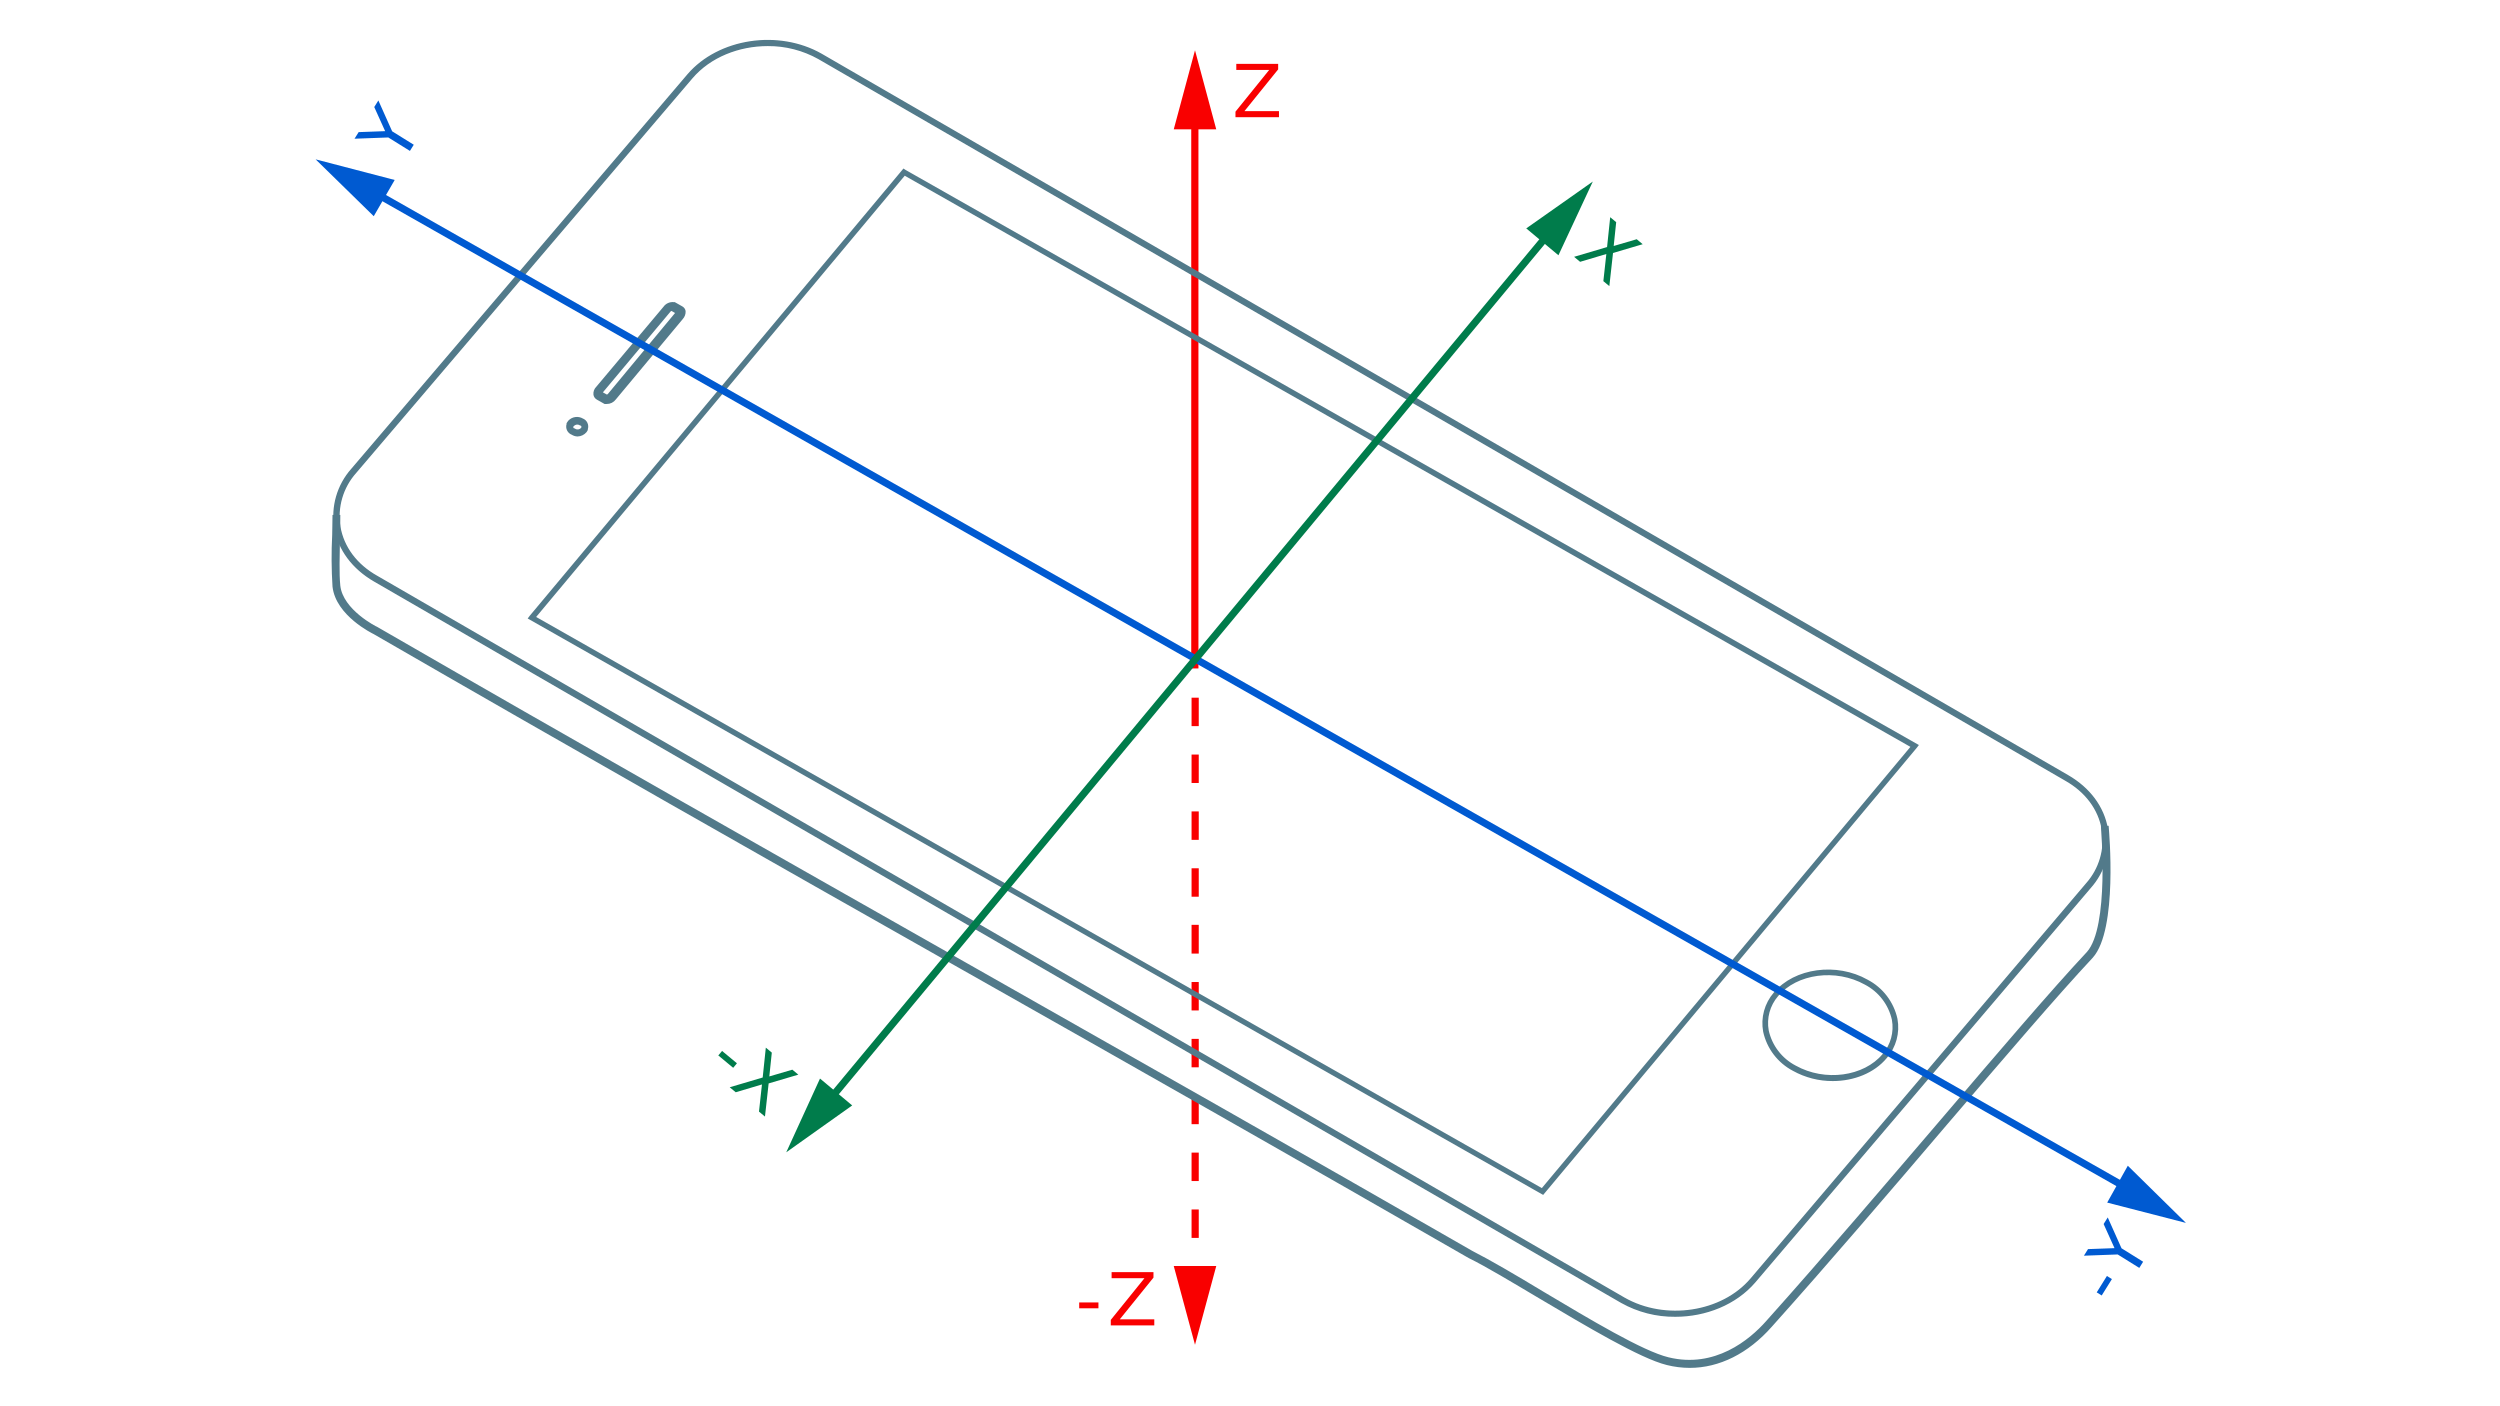
\includegraphics[width=0.6\textwidth, keepaspectratio]{imaxes/accelerometer_coordinate_system.png}
    \caption{Sistema de coordenadas del acelerómetro}
    \label{fig:accelerometer_coordinate_system}
\end{figure}


\subsection{Giroscopio}
Este sensor~\cite{gyroscope_draft} es capaz de medir la rotación del dispositivo en los tres ejes espaciales~[Figura~\ref{fig:gyroscope_sensor_coordinate_system}]. Es decir, nos ofrece la posición exacta en la que se encuentra el dispositivo.
\begin{figure}[h]
    \centering
    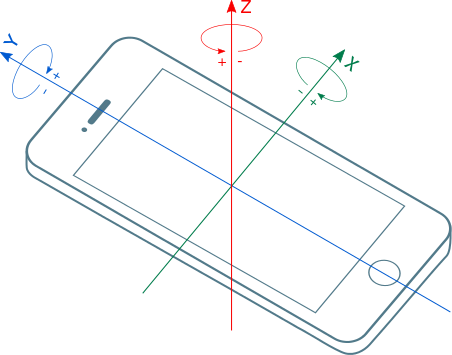
\includegraphics[width=0.5\textwidth, keepaspectratio]{imaxes/gyroscope_sensor_coordinate_system.png}
    \caption{Sistema de coordenadas del giroscopio}
    \label{fig:gyroscope_sensor_coordinate_system}
\end{figure}

\subsection{Extracción de características}
Los sensores mencionados anteriormente ofrecen los datos de un espacio tridimensional. Es decir, nos ofrecen tres valores correspondientes a cada uno de los ejes del espacio.
Debido a que ambos son dependientes de la posición, se ha decidido calcular una cuarta dimensión que no le afecte dicha posición, este nuevo valor es la magnitud que se calcula de la siguiente manera:

\begin{equation}
\texttt{magnitude} = \sqrt{ x^2 + y^2 + z^2}
\end{equation}
Para cada uno de estos cuatro valores obtenidos se han calculado nuevos valores~[Tabla~\ref{tab:sensor_features}] en ventanas de tiempo de cinco segundos. Estos valores, con ventanas de cinco segundos, han sido utilizados en otros estudios~\cite{ehatisham2018continuous} con buenos resultados. 

\begin{table}[H]
    \centering
    \begin{tabular}{l p{0.6\linewidth}}
    \toprule
    Nombre & Descripción \\
    \midrule
        \textbf{Media} &   Es un medida con tendencia al valor central. \\
        \textbf{Desviación estándar} &  Mide cuánto se separan los datos con respecto a la media aritmetica. \\
        \textbf{Varianza} &   Es el valor de la desviación estándar al cuadrado \\
        \textbf{Mínimo} &   Es el valor mínimo del conjunto. \\
        \textbf{Máximo} &   Es el valor máximo del conjunto. \\
        \textbf{Skewness} &   Es una variable que indica la asimetría de la distribución frente a la media. \\
        \textbf{Kurtosis} &   Es una variable que muestra la frecuencia de los datos. \\
    \bottomrule
    \end{tabular}
    \caption{Características de los sensores}
    \label{tab:sensor_features}
\end{table}

\section{Características del uso de la pantalla táctil}
La mayoría de los dispositivos de hoy en día son táctiles y, por lo tanto cuentan con una pantalla que es capaz de generar información sobre la interacción que el usuario realiza. Esta información~\cite{touch_events} extraída se calcula en base a la posición y tiempo entre el primer y último contacto con la pantalla.

A partir de la concatenación de varios de estos eventos en el tiempo, se pueden llegar a extraer otros más complejos como arrastrar, rotar\dots~ Para este proyecto se han capturado los mostrados en la Tabla~\ref{tab:event_type}.

\begin{table}[!h]
    \centering
    \begin{tabular}{l l p{0.6\linewidth}}
    \toprule
    Número de puntos & Nombre & Descripción \\
    \midrule
\multirow{4}{*}{Un sólo punto} & \textbf{Swipe} &   Es el movimiento de deslizamiento. \\
                                  & \textbf{Tap} &  Tocar la pantalla durante un corto periodo de tiempo \\
                                  & \textbf{Press} &  Tocar la pantalla durante un largo periodo de tiempo. \\
                                  & \textbf{Pan} &  Es el movimiento de arrastrar. \\
\midrule
\multirow{2}{*}{Dos puntos}  & \textbf{Pinch} &  Es el movimiento de juntar o separar los dedos para hacer zoom. \\
                                & \textbf{Rotate} &  Es el movimiento de girar los dedos para hacer rotar un objeto. \\
    \bottomrule
    \end{tabular}
    \caption{Tipos de eventos}
    \label{tab:event_type}
\end{table}

Como los eventos \textit{press} son poco frecuentas en cualquier tipo de aplicación se ha decidido descartarlos para el análisis.  Los eventos de \textit{pinch} y \textit{rotate} se han unido en un solo evento, puesto que ambos generan las mismas características. Este nuevo evento generado se ha llamado \textit{multitouch}.
La Tabla~\ref{tab:event_features} muestra las características extraídas para cada tipo de evento, que serán utilizadas para el análisis.


\begin{center}
    \begin{longtable}{l l p{0.6\linewidth}}
    \toprule
    Ev. & Nombre & Descripción \\
    \midrule
\multirow{8}{*}{\rotatebox[origin=c]{90}{Swipe}} & \textbf{duration}       & Duración del evento en milisegundos \\
                       & \textbf{distance}       & Distancia recorrida del evento en píxeles \\
                       & \textbf{velocity}       & Velocidad media del evento en píxeles/milisegundos  \\
                       & \textbf{angle}          & Ángulo creado desde el punto inicial al punto final \\
                       & \textbf{width}          & Ancho del área de pulsación en píxeles \\
                       & \textbf{height}         & Alto del área de pulsación en píxeles \\
                       & \textbf{frame\_index}   & Posición en la pantalla donde ha ocurrido el evento \\
                       & \textbf{direction}      & Dirección del evento \\
\midrule
\multirow{5}{*}{\rotatebox[origin=c]{90}{Tap}}   & \textbf{duration}       & Duración del evento en milisegundos \\
                       & \textbf{distance}       & Distancia recorrida del evento en píxeles \\
                       & \textbf{width}          & Ancho del área de pulsación en píxeles \\
                       & \textbf{height}         & Alto del área de pulsación en píxeles \\     
                       & \textbf{frame\_index}  & Posición en la pantalla donde ha ocurrido el evento \\
\midrule

\multirow{11}{*}{\rotatebox[origin=c]{90}{Pan}}  
& \textbf{duration} & Duración del evento en milisegundos \\
& \textbf{distance} & Distancia recorrida del evento en píxeles \\
& \textbf{velocity} & Velocidad media del evento en píxeles/milisegundos \\
& \textbf{angle} & Ángulo creado desde el punto inicial al punto final \\
& \textbf{width}              & Ancho del área de pulsación en píxeles \\
& \textbf{height}             & Alto del área de pulsación en píxeles\\ 
& \textbf{angle\_total}       & Suma de los ángulos realizados a lo largo del recorrido.\\ 
& \textbf{velocity\_y}        & Suma total de las velocidades a lo largo del recorrido, sobre el eje Y. \\
& \textbf{velocity\_x}        & Suma total de las velocidades a lo largo del recorrido, sobre el eje X. \\ 
& \textbf{avg\_velocity\_x}   & Velocidad media en el eje X \\ 
& \textbf{avg\_velocity\_y}   & Velocidad media en el eje Y \\ 
\midrule
\multirow{15}{*}{\rotatebox[origin=c]{90}{Multitouch}}  & \textbf{area}            & Área cubierta del evento, tomando como vértices los puntos mínimos y máximos de los dedos \\ 
                              & \textbf{abfs}            & Ángulo entre los dos primeros puntos\\ 
                              & \textbf{abfe}            & Ángulo entre los dos últimos puntos\\ 
                              & \textbf{rbfs}            & Distancia entre los dos primeros puntos eje y\\ 
                              & \textbf{rbfe}            & Distancia entre los dos primeros puntos eje x\\ 
                              & \textbf{df\_up}          & Distancia entre del dedo superior eje x\\ 
                              & \textbf{df\_dow}         & Distancia entre del dedo inferior eje x\\ 
                              & \textbf{avg\_width\_0}   & Ancho del área de pulsación en píxeles\\ 
                              & \textbf{avg\_width\_1}   & Ancho del área de pulsación en píxeles\\ 
                              & \textbf{avg\_height\_0}  & Alto del área de pulsación en píxeles\\ 
                              & \textbf{avg\_height\_1}  & Alto del área de pulsación en píxeles\\ 
                              & \textbf{velocity\_dow}   & Velocidad media del dedo inferior\\ 
                              & \textbf{velocity\_up}    & Velocidad media del dedo superior\\ 
                              & \textbf{duration}        & Duración del evento en milisegundos\\ 
                              & \textbf{direction}      & Dirección del evento \\

    \bottomrule
    \caption{Características por tipo de evento}
    \label{tab:event_features}
    \end{longtable}
\end{center}



\section{Evaluación del rendimiento}
\label{sec:metrics}

Para analizar los resultados obtenidos y comprobar la fiabilidad de los algoritmos usados, necesitamos emplear unas métricas que evalúen su rendimiento y permitan comparar diferentes aproximaciones.

Al ser este un problema de clasificación binaria (usuarios legítimos, usuarios no legítimos) se ha utilizado la matriz de confusión~[Figura~\ref{fig:matrix_conf}], la cual categoriza los datos en cuatro grupos:


\begin{itemize}
    \item \textbf{Verdaderos Negativos (TN)}: Es la cantidad de negativos que fueron clasificados correctamente como negativos.
    
    \item \textbf{Falsos Positivos (FP)}: Es la cantidad de negativos que fueron clasificados incorrectamente como positivos.
    
    \item \textbf{Falsos Negativos (FN)}: Es la cantidad de negativos que fueron clasificados incorrectamente como negativos.
    
    \item \textbf{Verdaderos Positivos (TP)}: Es la cantidad de positivos que fueron clasificados correctamente como positivos.
\end{itemize}


\begin{figure}[H]
    \centering
    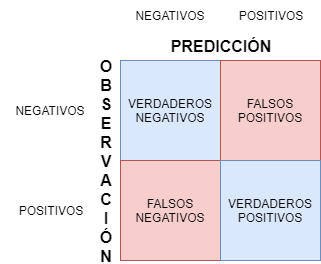
\includegraphics[width=0.5\textwidth, keepaspectratio]{imaxes/matriz_confusion.png}
    \caption{Esquema matriz de confusión}
    \label{fig:matrix_conf}
\end{figure}

A partir de los datos obtenidos de una matriz de confusión, se pueden calcular medidas que permiten obtener una representación analítica de los resultados. Por otra parte, durante el entrenamiento de los algoritmos también se han calculado los tiempos de cómputo.

\begin{itemize}
    \label{list:scores}
    \item\textbf{Recall (RC)}: Es la relación entre las predicciones positivas correctas y el total de observaciones positivas.
        \begin{equation}
            \frac{TP}{TP + FN}
        \end{equation}
    
    \item \textbf{Precision (PS)}: Es la relación entre las predicciones positivas correctas y el total de predicciones positivas.
        \begin{equation}
            \frac{TP}{TP  + FP}
        \end{equation}
    
    \item \textbf{F1}: Es la media armónica de los valores anteriores. 
        \begin{equation}
            \frac{2}{\frac{1}{precision} + \frac{1}{recall}} = 2 * \frac{precision * 
    recall}{precision + recall} = \frac{TP}{TP + \frac{FN + FP}{2}}
        \end{equation}
    
    \item \textbf{Accuracy}: Es la relación entre las predicciones positivas y el total de casos.
        \begin{equation}
            \frac{TP}{TP + FP + FN + TN} 
        \end{equation}
    
    
    \item \textbf{Fit Time}: Tiempo de cómputo que ha tardado en entrenar el algoritmo.
    
    \item \textbf{Score Time}: Tiempo de cómputo que ha tardado en ejecutar la predicción.
\end{itemize}

Para analizar los resultados, se ha favorecido el uso de la métrica \textit{precision} para tratar de minimizar posibles intrusiones.



\section{Inteligencia Artificial}

En 1956, \textbf{Jhon McCarthy}~\cite{jhonmccarthy}, conocido como el padre de la Inteligencia Artificial, acuñó el término Inteligencia Artificial, en adelante \textit{IA}, como la ciencia y la ingeniería de hacer máquinas inteligentes, especialmente programas informáticos inteligentes.

En la \textit{IA} existen dos grupos definidos, fuerte y débil. La  \textit{IA} fuerte es aquella que tiene las mismas características que un humano inteligente. La \textit{IA} débil es aquella que muestra inteligencia en un área en concreto pero carece de la misma en otras.

Para conseguir dotar de inteligencia a una máquina se suele utilizar el aprendizaje máquina o \textit{machine learning}. El aprendizaje máquina, en adelante \textit{ML}, es una de las áreas más extendidas de la \textit{IA}. En 1959, \textbf{Arthur Samuel}~\cite{arhtursamuel} definió \textit{ML} como el campo de estudio que brinda a las computadoras la capacidad de aprender sin estar programado explícitamente.

\subsection{Tipo de aprendizaje}

Dentro del \textit{ML} se pueden distinguir dos tipos de aprendizaje:

\begin{itemize}
    \item \textbf{Aprendizaje supervisado}: Los algoritmos son entrenados en base a un conjunto de datos de los que conocemos su respuesta correcta. De esta manera lo que se intenta es que el algoritmo obtenga la respuesta correcta a partir de las características disponibles.
    
    \begin{itemize}
        \item \textbf{Problemas de regresión}: Son usados para evaluar las relaciones que existen entre las variables y obtener un valor de esa estimación.
        \item \textbf{Problemas de clasificación}: Son utilizados para dividir un conjunto de datos de entrada en distintas clases según sus características.
    \end{itemize}
    
    \item \textbf{Aprendizaje no supervisado}: En este modelo, los datos no contienen una respuesta correcta. Este tipo de aprendizaje intenta buscar ciertos patrones o respuestas, pero no una respuesta concreta.
\end{itemize}

%En este proyecto se ha usado el aprendizaje supervisado para clasificar nuestros datos en función de las características extraídas y de esta manera decidir si un usuario es legítimo o no.

La finalidad de todos estos tipos de aprendizajes es la de generalizar, es decir, que puedan resolver problemas que no han visto. 
Cuando entrenamos modelos computacionales con un conjunto de datos de entrada estamos haciendo que el algoritmo sea capaz de generalizar un concepto para que al consultarle por un nuevo conjunto de datos desconocido este sea capaz de comprenderlo y proporcionarnos un resultado fiable~[Figura~\ref{fig:over-under-fitting}].

Si nuestros datos de entrenamiento son muy pocos o poco representativos nuestra máquina no será capaz de generalizar el conocimiento y estará incurriendo en \textit{underfitting}~[Figura~\ref{fig:over-under-fitting}].

Si sobrentrenamos nuestro modelo lo que ocurrirá es que nuestra máquina sólo se limitará a memorizar los casos particulares que le enseñamos y será incapaz de reconocer nuevos datos de entrada, perdiendo toda capacidad de generalización.



\begin{figure}[h]
    \centering
    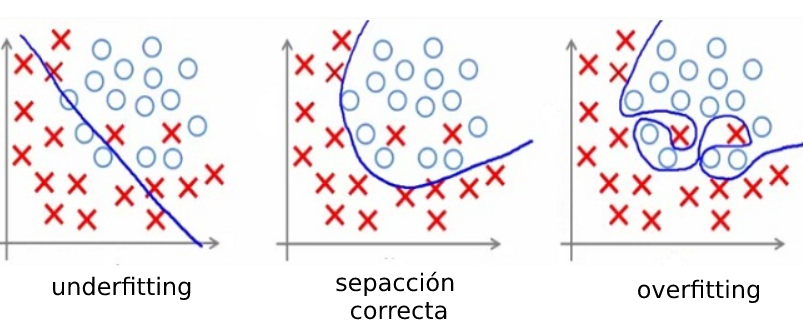
\includegraphics[width=0.7\textwidth, keepaspectratio]{imaxes/overfitting.png}
    \caption{Problemas de entrenamiento}
    \label{fig:over-under-fitting}
\end{figure}


% ======================================================== %

% ======================================================== %

\subsection{Redes Neuronales Artificiales}
Las redes neuronales artificiales~\cite{salas2004redes}, en adelante \textit{RNA}, son un modelo computacional inspirado en la estructura del sistema nervioso de los seres humanos. La unidad elemental de una \textit{RNA} es la neurona artificial [Figura~\ref{fig:neurona}] y generalmente están organizadas en capas. Poseen varias entradas y una salida, que se calcula normalmente realizando una suma ponderada de las entradas con sus pesos~[\ref{eq:perceptron}]. 

\begin{equation} \label{eq:perceptron}
    \displaystyle\sum_{i=1}^{n} w_i x_i + w_0= 
    \begin{cases}
        \geq 0       & \quad y = 1 \\
        <    0       & \quad y = 0
    \end{cases}
\end{equation}

Este resultado es modificado por una función de activación y el valor obtenido se transmite directamente al siguiente elemento. Normalmente para conseguir esta transformación se emplean funciones como la sigmoidal, gaussiana o la tangente hiperbólica:

\begin{itemize}
    \item Función sigmoidal: 
    \begin{equation}
        f(x) = \frac{1}{1 + e^{-x}}
    \end{equation}
    
    \item Función tangente hiperbólica: 
    \begin{equation}
        f(x) = tanh(x)
    \end{equation}
    
    \item Función gaussiana: 
    \begin{equation}
        f(x) = e^{\frac{-x^2}{2}}
    \end{equation}
    
    
\end{itemize}



\begin{figure}[H]
    \centering
    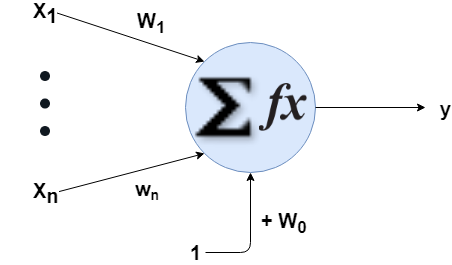
\includegraphics[width=0.7\textwidth, keepaspectratio]{imaxes/neurona.png}
    \caption{Esquema de un neurona artificial}
    \label{fig:neurona}
\end{figure}







% ======================================================== %

% ======================================================== %

\subsection{Perceptrón Multicapa}
\label{sec:mlp}

En 1958, \textbf{Rosenblatt}~\cite{rosenblatt1960perceptron} diseñó y desarrollo el perceptrón. Este modelo implementa el funcionamiento de una sola neurona que es capaz de resolver problemas lineales. En 1969, \textbf{Minsky y Papert} escribieron un libro~\cite{minsky2017perceptrons} donde demostraron que un solo perceptrón era incapaz de aprender la función exclusiva (XOR), es decir, problemas cuya resolución no es lineal. En este mismo libro se expone un nuevo paradigma de \textit{RNA} llamado perceptrón multicapa  también conocido como \textit{MLP} por sus siglas en inglés (\textit{Multi-Layer Perceptron}). Este modelo es una combinación de varios perceptrones, que permiten aproximar cualquier problema, aunque no sea lineal. Éste se caracteriza por tener sus neuronas agrupadas en capas de diferentes niveles, por lo general tres~[Figura~\ref{fig:schematic_MLP}]. 

\begin{itemize}
    \item \textbf{Capa de entrada }: Esta capa conecta la red con el exterior, cada neurona se corresponde con cada una de las variables de entrada a la red.
    
    \item \textbf{Capas ocultas }: Es un conjunto de capas que cuyas entradas son las salidas de la capa anterior y cuya salida pasan a la capa sucesora.
    
    \item \textbf{Capa de salida }: Conecta las capas ocultas con la salida de la red que proporciona los resultados.
\end{itemize}

Además, sus conexiones están dirigidas hacia adelante, es decir, las neuronas de una capa se conectan con las neuronas de la siguiente capa y generalmente todas las neuronas de una capa se encuentran enlazadas con las de la siguiente capa.


\begin{figure}[H]
    \centering
    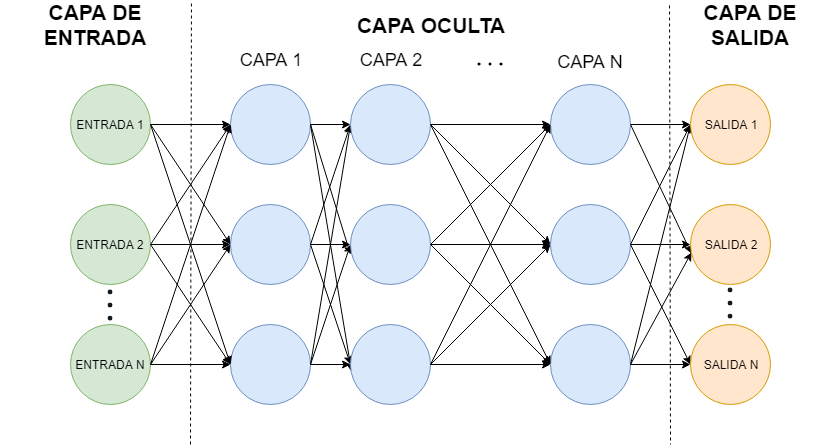
\includegraphics[width=0.9\textwidth, keepaspectratio]{imaxes/schematic_mlp.png}
    \caption{Esquema del MLP}
    \label{fig:schematic_MLP}
\end{figure}

Inicialmente, este planteamiento no se pudo materializar porque no existía un mecanismo que ajustase automáticamente los pesos de la capa oculta. En 1986, \textbf{Rummelhart, Hinton y Wiliams} desarrollan la \textit{Regla Delta Generalizada}~\cite{rumelhart1988learning} para adaptar los pesos propagando los errores hacia atrás. De esta manera se demuestra que el \textit{MLP} es capaz de resolver problemas lineales y no lineales.

En la Figura~\ref{fig:MLP_example} se puede ver el funcionamiento del \textit{MLP}. En ella se muestra el esquema de un \textit{MLP} que contiene una capa de entrada, dos capas ocultas y la salida. 
Cada neurona está representada visualmente con una gráfica que muestra la función aplicada a los datos, por ejemplo, en la capa de entrada, las variables de entrada son dos funciones que dividen los datos en vertical~($X_1$) y horizontal~($X_2$). También se pueden observar la distintas conexiones que existen entre las neuronas e incluso el peso de las conexiones representadas por un color y grosor diferentes.

\begin{figure}[!h]
    \centering
    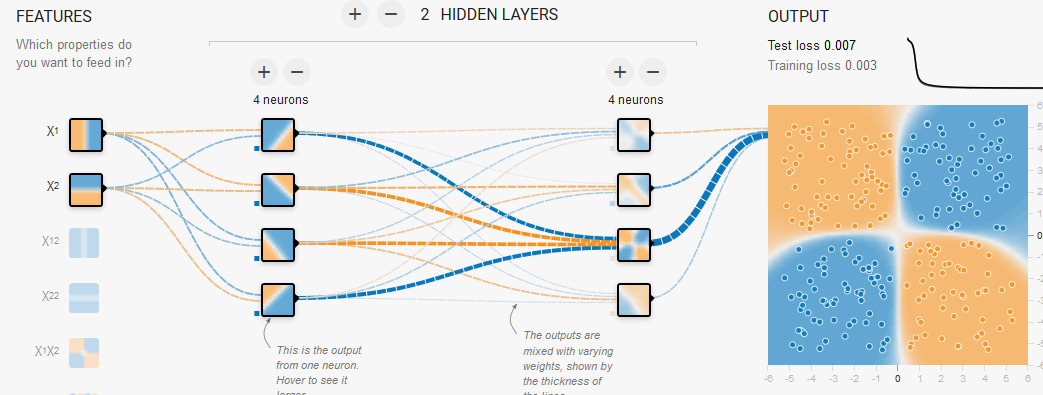
\includegraphics[width=0.9\textwidth, keepaspectratio]{imaxes/MLP_example.png}
    \caption[Ejemplo de una MLP]{Ejemplo de una MLP~\cite{tensorflow}}
    \label{fig:MLP_example}
\end{figure}


Este tipo de arquitectura es muy utilizada debido a su capacidad de aproximación universal. No obstante, requieren un largo proceso de aprendizaje para problemas complejos que requieren de un gran número de variables y una arquitectura compleja.


% ======================================================== %

% ======================================================== %

\subsection{Maquinas de soporte vectorial}
\label{sec:svm}
Las máquinas de soporte vectorial~\cite{berwick2003idiot} también conocidas como \textit{SVMs} de sus siglas en inglés (\textit{Support Vector Machines}), es un conjunto de algoritmos desarrollados por \textbf{Vladimir Vapnik}, capaces de realizar clasificaciones, regresiones e incluso detectar valores atípicos. 


Las \textit{SVMs} generan un hiperplano\footnote{Es un plano de una dimensión inferior al origen, que divide el espacio en dos mitades} para intentar clasificar los datos [Figura~\ref{fig:svm_example}]. En dicho hiperplano se forma una \textit{calle} para separar los datos, donde la línea continua separa el conjunto y las líneas discontinuas indican el margen de error. Las \textit{SVMs} intentan maximizar el margen de error, lo que ocasiona una \textit{calle} más grande y por lo tanto generalizará mejor el problema.

\begin{figure}[h]
    \centering
    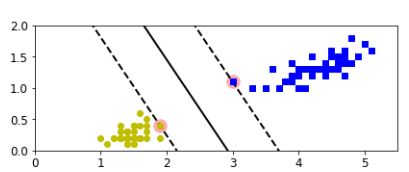
\includegraphics[width=0.7\textwidth, keepaspectratio]{imaxes/svm_exmaple.png}
    \caption{Ejemplo de Clasificación SVM}
     \label{fig:svm_example}
\end{figure}


\subsubsection{Tipos de problemas}

El conjunto de datos utilizados por estos algoritmos suelen ser multidimensionales, por lo tanto, en ciertas ocasiones puede ser complicado separar los datos. En base a esto podemos encontrarnos con dos tipos de escenarios:

\begin{itemize}
    \item \textbf{Lineales~[Figura~\ref{fig:svm_example}] } : La solución de este tipo de problemas genera un hiperplano que es capaz de separar el conjunto de datos perfectamente.
    
    \item \textbf{No lineales}: Son aquellos en los que el conjunto de entrada no es posible separarlos con un hiperplano, pero el hecho de que no sean separables en el espacio original, no significa que no lo sean en un espacio de dimensiones distinto. Para transformar el espacio de entradas a una dimensión diferente se emplean las funciones kernel:
    \begin{itemize}
    \item \textbf{Lineal} : Kernel utilizado cuando pretendemos aproximar nuestra función con una función lineal.
        \begin{equation}
            K(x,y) =  x y + c
        \end{equation}
        donde $c$ es una constante.
    \item \textbf{Polinómica}: Representa la similitud de los vectores en un espacio polinómico distinto al original.
        \begin{equation}
            K(x,y) = (a + xy)^d
        \end{equation}
    donde $d$ es el orden del polinomio y $a$ es una constante.

    \item \textbf{Función de base radial Gaussiana (RBF )~[Figura~\ref{fig:kernel_clf}]}: Genera un nuevo espacio calculando las distancias entre un puntos concreto y el resto de puntos.
    
    \begin{equation}
        K(x,y)=exp(- \frac{||x-y||^2}{2\sigma^2})
    \end{equation}
    
    donde $\sigma$ es la anchura del kernel y $||x-y||$ es la distancia euclídea\footnote{es la distancia entre dos puntos de un espacio euclídeo, la cual se deduce a partir del teorema de Pitágoras.} entre $x$ e $y$ 

    \item \textbf{Función sigmoide}: Aplica la función sigmoide para generar un nuevo espacio de valores.
        \begin{equation}
            K(x,y)=tanh(\alpha x y+ c)   
        \end{equation}
    donde $\alpha$ es la pendiente y $c$ es una constante.
    \end{itemize}
\end{itemize}



\begin{figure}[H]
    \centering
    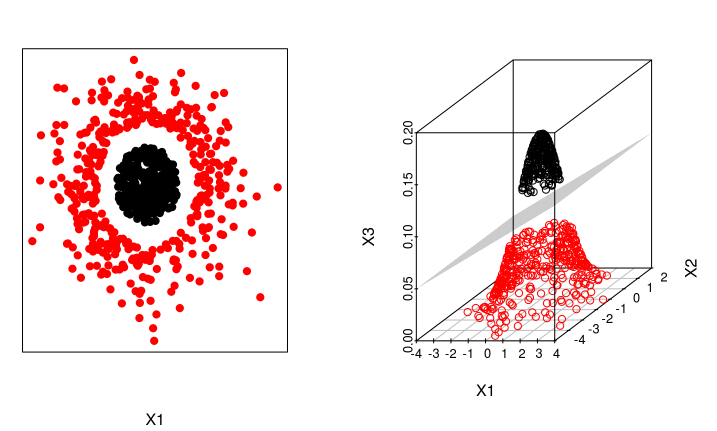
\includegraphics[width=0.7\textwidth, keepaspectratio]{imaxes/svm_exmaple_clf.png}
    \caption[Ejemplo de Clasificación SVM no lineal, usando función gaussiana]{Ejemplo de Clasificación SVM no lineal, usando función gaussiana \cite{joaquin}}
     \label{fig:kernel_clf}
\end{figure}

\subsection{Árboles de Decisión}
\label{sec:decision_tree}
Generan modelos de clasificación o regresión usando árboles como estructuras internas~[Figura~\ref{fig:decisiontree}]. En dicha estructura cada nodo representa una característica del problema, cada rama representa una decisión de esa característica y los nodos hoja contienen el valor de la predicción o clase.

\begin{figure}[h]
    \centering
    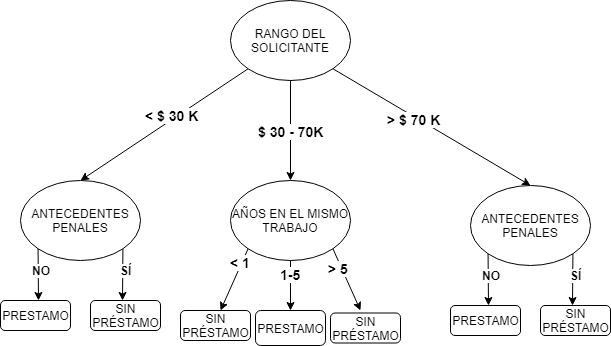
\includegraphics[width=0.7\textwidth, keepaspectratio]{imaxes/decision_tree.png}
    \caption{Árbol de decisión para conceder un préstamo}
    \label{fig:decisiontree}
\end{figure}

\subsection{Regresión Logística}
\label{sec:logistic_regresion}
Es un algoritmo de clasificación usado para asignar un conjunto de valores a dos tipos de clases. 
Para obtener el valor de la predicción utiliza la función sigmoide.

\begin{equation}
    \label{eq:sigmoide}
    S(x) = \frac{1}{1+e^{-x}}
\end{equation}

\subsection{\textit{k-Nearest Neighbours}}
\label{sec:kn}
Es un método que busca en las observaciones más cercanas a la que se está tratando de predecir y clasifica en base a la mayoría de datos que lo rodean~[Figura~\ref{fig:k_n}]. Las técnicas utilizadas para calcular las distancias suelen ser distancia euclidiana, distancia Manhattan\dots

\begin{figure}[!h]
    \centering
    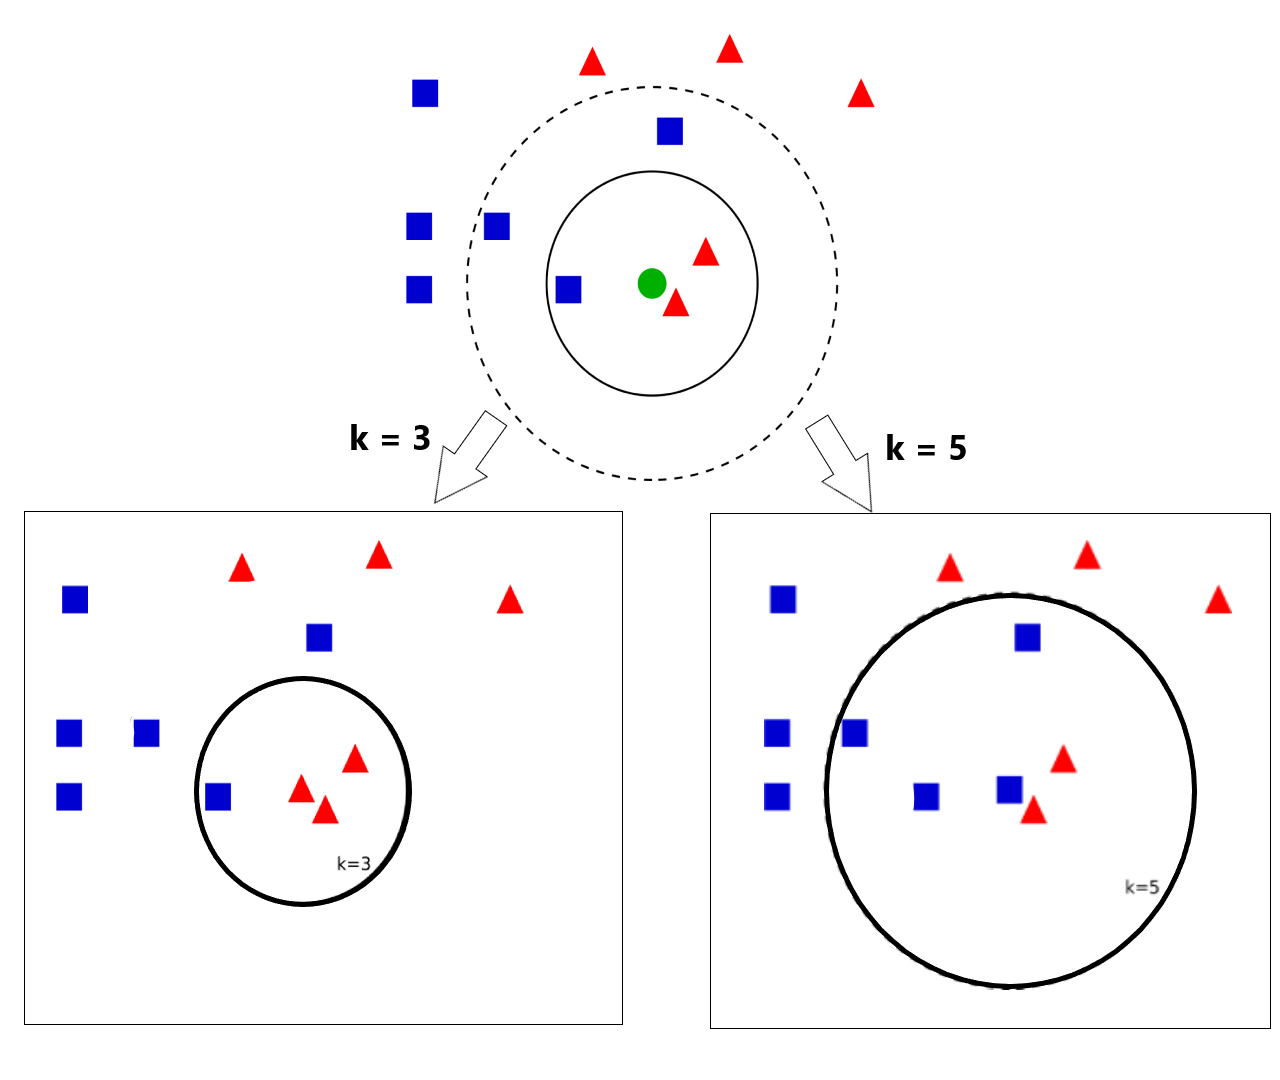
\includegraphics[width=0.7\textwidth, keepaspectratio]{imaxes/KnnClassification.png}
    \caption{Ejemplo de k-Nearest Neighbours}
    \label{fig:k_n}
\end{figure}

\subsection{Métodos Ensambladores}
Los métodos de tipo ensamblador están formados por un grupo de modelos predictivos que permiten alcanzar una mejor precisión y estabilidad del modelo. Estos utilizan diferentes técnicas para mejorar los resultados de un algoritmo, ya sea combinándolo con otros o utilizando varias instancias del mismo. 

Algunas de estas técnicas son \textit{Stacking}, \textit{Bagging} y \textit{Boosting}. Estas dos últimas utilizan \textit{Bootstrapping} como método de muestreo de datos.

\subsubsection{\textit{Bootstrapping}}
Es un técnica de muestreo. De las \textit{n} muestras disponibles, se escogen \textit{k} con reemplazo. Luego ejecutamos nuestros algoritmos utilizando esas muestras. Se utiliza el remplazo para asegurar que las muestras sean aleatorias. Si se realizase sin remplazo, las muestras extraídas dependerán de las anteriores.

\begin{figure}[h]
    \centering
    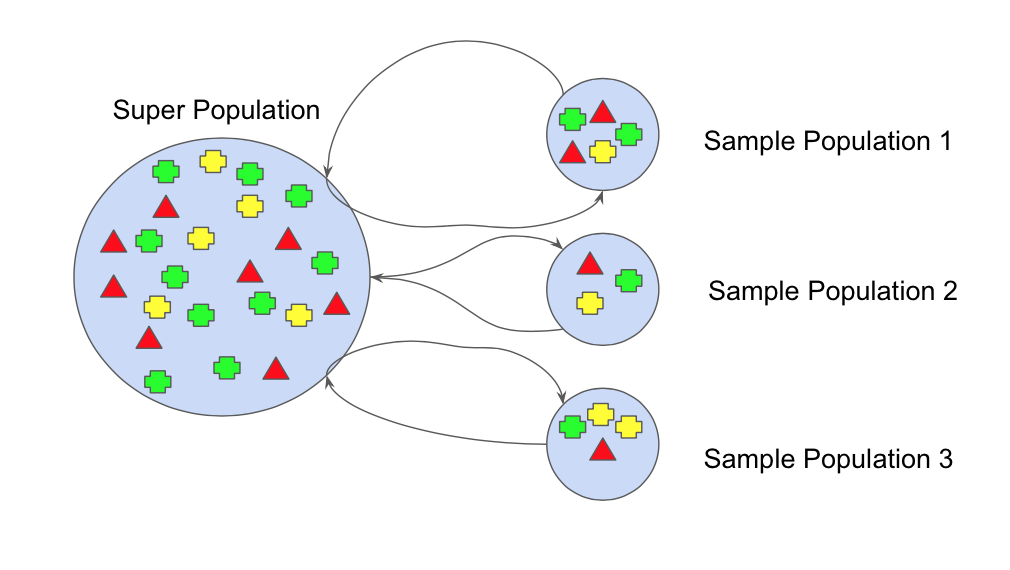
\includegraphics[width=0.7\textwidth, keepaspectratio]{imaxes/Bootstrapping.png}
    \caption[Ejemplo de \textit{Bootstrapping}]{Ejemplo de \textit{Bootstrapping}~\cite{Bootstrapping}}
    \label{fig:bootstrapping}
\end{figure}


\subsubsection{\textit{Bagging}~\cite{breiman1996bagging}}

Este método genera  múltiples instancias de un mismo modelo predictivo para conseguir una mejora en la precisión de la predicción. Generalmente esta técnica puede ser usada para reducir en algoritmos que tienen una alta varianza para reducirla.


\subsubsection{\textit{Boosting}}
Esta técnica emplea un conjunto de algoritmos que utilizan promedios ponderados para convertir aprendizajes débiles en fuertes. Cada modelo ejecutado, dicta en que características se centrará el siguiente modelo.

\begin{figure}[h]
    \centering
    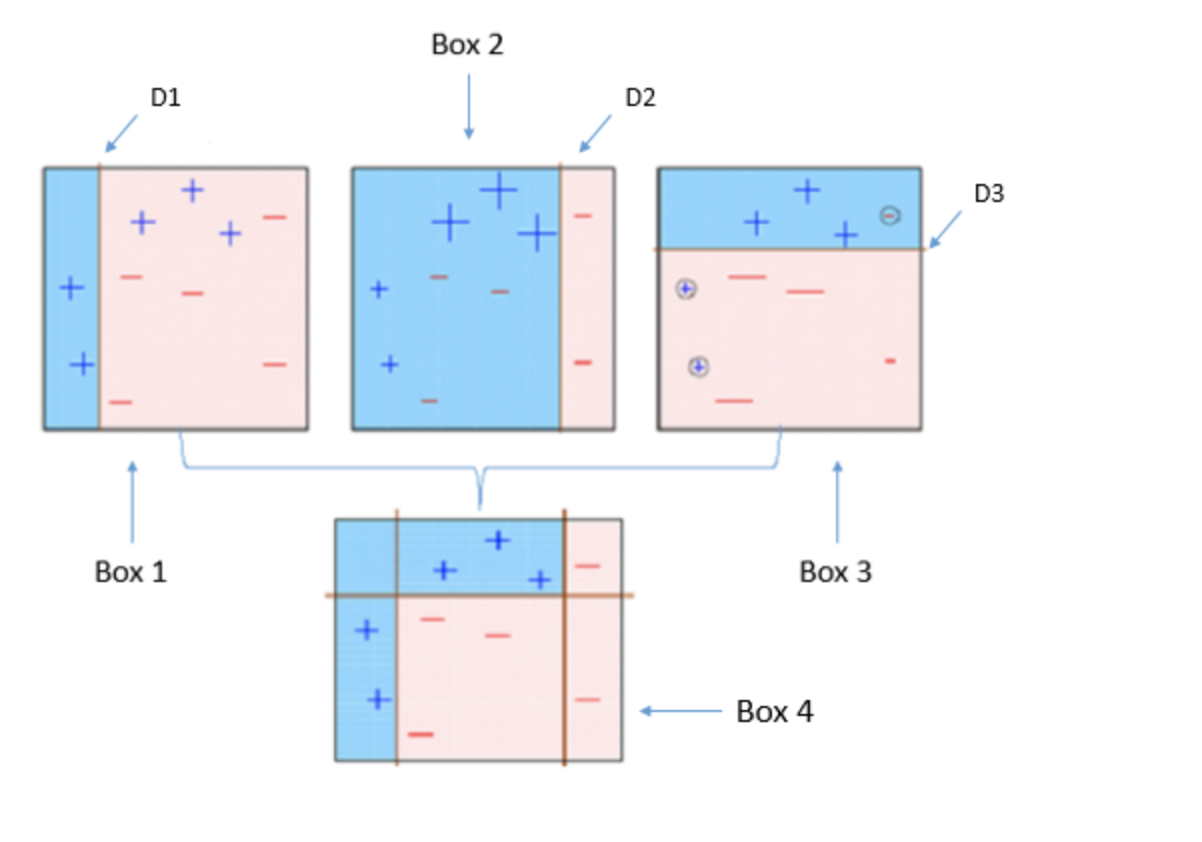
\includegraphics[width=0.7\textwidth, keepaspectratio]{imaxes/boosting.png}
    \caption[Ejemplo de \textit{Boosting}]{Ejemplo de \textit{Boosting}~\cite{bossting}}
    \label{fig:bossting}
\end{figure}

\subsubsection{\textit{Stacking}}
Esta técnica combina múltiples modelos de clasificación o regresión. Los modelos son entrenados individualmente utilizando un conjunto de entrenamiento y sus resultados son combinados para obtener una predicción final.

\subsection{Bosques Aleatorios}
\label{sec:random_forest}
Los bosques aleatorios~\cite{Breiman2001} también conocidos como \textit{Random Forest}, fueron desarrollados por \textbf{Leo Breiman} y \textbf{Adele Cutler}. Este algoritmo utiliza la técnica de \textit{Bagging} para realizar las predicciones.

Son un conjunto de árboles de decisión en el que cada árbol depende de los valores de un vector aleatorio probado independientemente y con la misma distribución para cada uno de los árboles del bosque [Figura~\ref{fig:schematic_RandomForest}].




\subsubsection{Ventajas}

Las ventajas de los \textit{Random Forest} son:

\begin{itemize}
    \item Es uno de los algoritmos de aprendizaje más fiables.
    \item Funciona bien con conjunto de datos muy grandes.
    \item Puede manejar cientos de variables de entrada.
    \item Guarda la información sobre las variables más importantes.
\end{itemize}

\subsubsection{Desventajas}

\begin{itemize}
    \item No funcionan bien cuando hay variables categóricas.
    \item Puede sobre ajustar en ciertos grupos de datos con mucho ruido.
\end{itemize}



\begin{figure}[h]
    \centering
    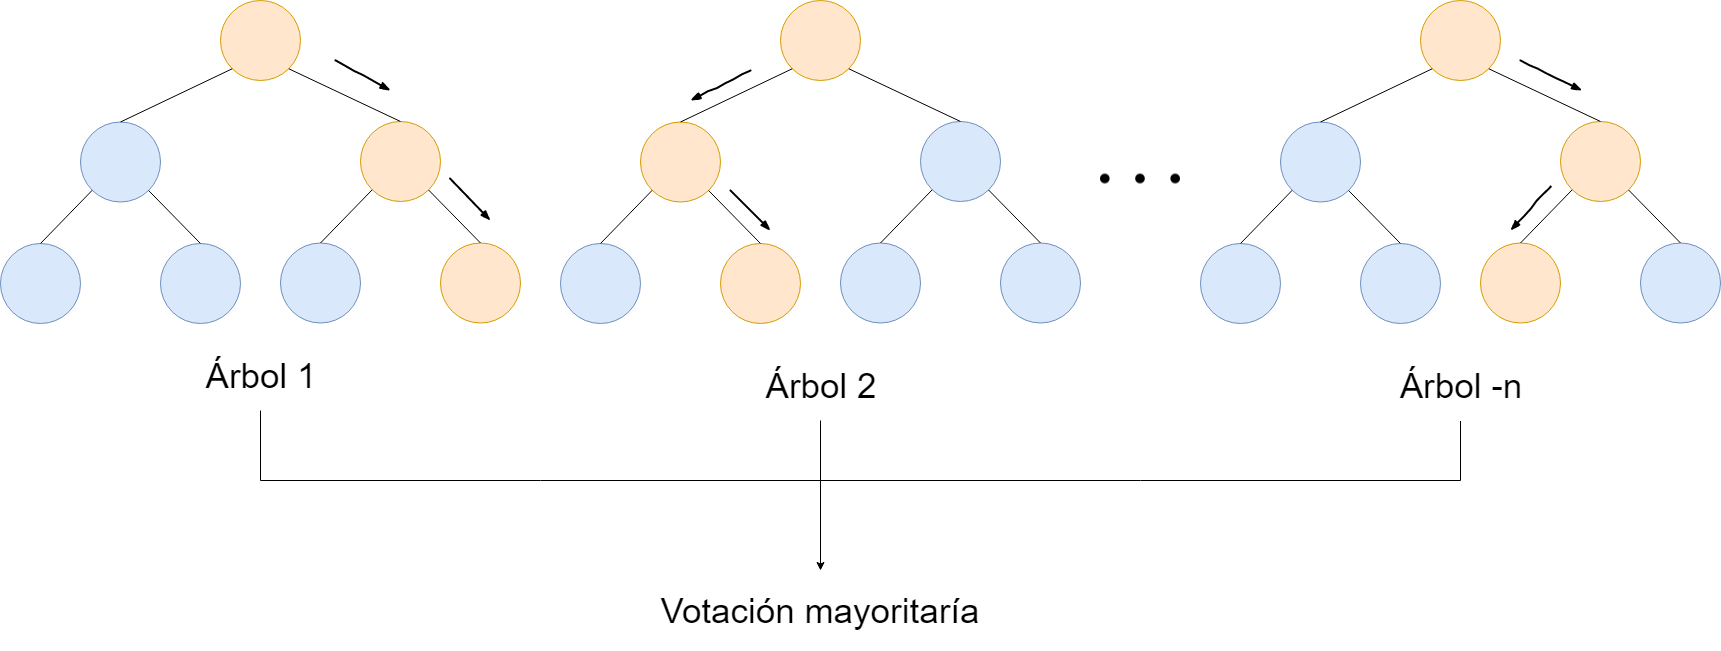
\includegraphics[width=0.9\textwidth, keepaspectratio]{imaxes/random_forest.png}
    \caption{Esquema \textit{Random Forest}}
    \label{fig:schematic_RandomForest}
\end{figure}



% ======================================================== %

% ======================================================== %


\subsection{Clasificador por Votación} 
\label{sec:voting_clf}

La clasificación por votación~\cite{voting_clf} es un meta-clasificador, es decir, no implementa un algoritmo de clasificación sino que evalúa las predicciones de otros algoritmos para obtener una nueva [Figura~\ref{fig:schematic_Voting}]. Este algoritmo se basa en la técnica de \textit{Stacking} para obtener las predicciones.

\subsubsection{Tipos de votación}

\begin{itemize}
    \item \textbf{Votación Dura/Mayoritaria} :  Es un caso de selección por mayoría simple. La predicción se hace en base al mayor número de votos por parte de los algoritmos utilizados.
    
    \item \textbf{Votación Blanda} : Esta técnica calcula el mejor resultado obteniendo la media de las probabilidades calculadas por los algoritmos individualmente.
\end{itemize}

\subsubsection{Ventajas}

\begin{itemize}
    \item Por norma general suelen proporcionar mejores resultados, si se rigen por ciertas condiciones, como que los clasificadores sean totalmente independientes~\cite{RUTA200563}.
\end{itemize}

\subsubsection{Desventajas}

\begin{itemize}
    \item No todos los algoritmos son válidos para esta técnica, especialmente cuando se usa el método de votación blanda, ya que no todos los algoritmos estiman las probabilidades de las salidas.
\end{itemize}


\begin{figure}[h]
    \centering
    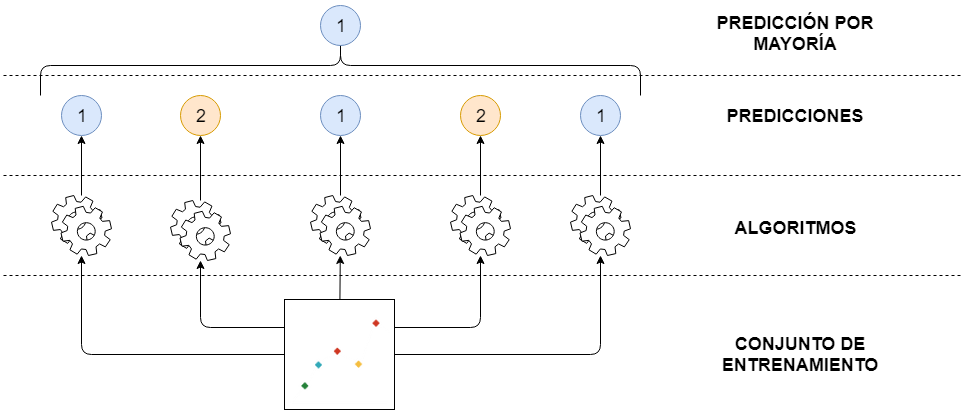
\includegraphics[width=1\textwidth, keepaspectratio]{imaxes/schema_voting.png}
    \caption{Esquema clasificación por votación}
    \label{fig:schematic_Voting}
\end{figure}

 \section{Estudio de alternativas}
\label{Estudio de alternativas}
Debido al interés de este tipo de sistemas de autenticación, se pueden encontrar múltiples estudios relacionados. Existen un número importante de estudios/proyectos sobre la autenticación basada en el uso de un dispositivo móvil y los sensores que este contiene. Pero la mayoría de estos estudios/proyecto no consiguen obtener un producto final~\cite{EHATISHAMULHAQ201824}~\cite{JAIN2019604}~\cite{DAMOPOULOS2019138}~\cite{SMITHCREASEY2018147}~\cite{YANG20199}. 

Las alternativas que tienen o muestran un producto final usable se mencionan en las siguientes secciones del capitulo.

\subsection{SealSign}

En el \textit{Mobile World Congress} del año 2015 se dio a conocer \textit{SealSign}~\cite{sealsign} por \textbf{Eleven Paths}, una aplicación que permite la firma manuscrita en los dispositivos móviles, mediante el análisis de parámetros biométricos para validar al usuario. Estos parámetros, según los desarrolladores, son la velocidad y la presión en los ejes X e Y, de los cuales obtienen la huella biométrica de esa firma. Este sistema cuenta con la posibilidad de realizar firmas masivas de documentos y, además, permite una integración con cualquier otro lenguaje de manera sencilla.


\subsection{Biosig-id}
\textit{Biosig-id}~\cite{biosig-id} es una herramienta de seguridad que no solo valida la contraseña del usuario, sino que además analiza el comportamiento de escritura tanto con ratón como por pantalla táctil. Esta herramienta cuenta con aplicación de demostración~\footnote{\url{https://biosig-id.com/go-verify-yourself/}} en la que retan al usuario a falsificar una firma, dando una recompensa al que consiga entrar.


\subsection{Touch me once and I know it's you }

En el año 2012 un grupo de la Universidad de Múnich, desarrolló una aplicación~\cite{de2012touch} que capturaba los movimientos del usuario cuando estos realizaban el patrón para desbloquear el móvil. La aplicación consistía en repetir ochenta veces seguidas el patrón de desbloqueo, para evitar la monotonía del proceso, se realizaban pausas cada veinte patrones, en las cuales el usuario debía de realizar otro tipo de acciones durante un periodo largo de tiempo.





 \include{contido/planificación}
 \chapter{Tecnologías}
\label{chap:tecnologias}
A lo largo del capítulo se explicarán las tecnologías utilizadas para la realización del proyecto, así como otros aspectos relacionados con su desarrollo.

\section{Arquitectura}

Para comenzar a desarrollar un proyecto software hay que tener en cuenta qué herramientas vamos a usar y qué requisitos debemos cumplir. Por ello se necesita conocer cómo va a ser la estructura de alto nivel de nuestro proyecto para desarrollarla y de esta manera conseguir un sistema robusto y escalable. 

En este proyecto se ha utilizado una arquitectura de tres capas [Figura \ref{fig:arquitectura}] que se distribuye de la siguiente manera:

\begin{itemize}
    \item \textbf{Capa de Presentación:}  Presenta el sistema al usuario, le comunica la información y captura la información. Esta capa se comunica únicamente con la capa de negocio.    
    \item \textbf{Capa de Negocio:} Se reciben las peticiones del usuario y se envían las respuestas tras la ejecución. Se denomina capa de negocio porque es donde se establecen las reglas de procesado de los datos. Esta capa se comunica con la capa de presentación, para recibir solicitudes y enviar los resultados, y con la capa de datos, para solicitar el almacenamiento y recuperación de los datos.
    
    \item \textbf{Capa de Datos:}  Es donde residen los datos y es la encargada de acceder a los mismos. Está formada por uno o varios gestores de bases de datos que se encargan de procesar las solicitudes de almacenamiento o recuperación de información desde la capa de negocio.

\end{itemize}

Cada una de estas capas suele distribuirse en distintos servidores, aunque podría darse que todas las capas se encontrasen en uno solo. Este tipo de arquitectura permite replicar la capa que más lo necesite. Lo que otorga la capacidad de escalar la aplicación sobre las partes que se consideren más críticas. Es decir, si tenemos un sistema que necesita procesar muchas operaciones de guardado o lectura de datos, podríamos replicar la capa de datos en otros ordenadores balanceando las peticiones sobre los nuevos servicios creados.
\begin{figure}[H]
    \centering
    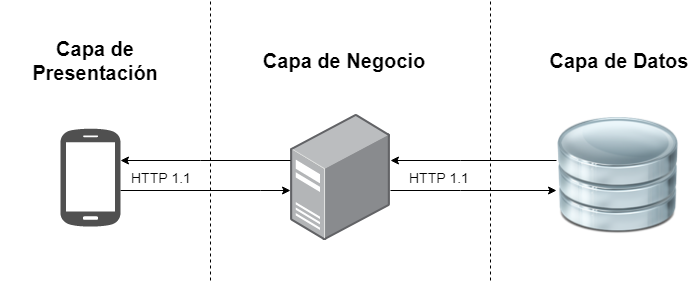
\includegraphics[width=0.7\textwidth, keepaspectratio]{imaxes/layer.png}
    \caption{Arquitectura de tres capas}
    \label{fig:arquitectura}
\end{figure}


\subsection{Capa de Presentación}
Para esta parte de la arquitectura se ha utilizado \textit{Angular} como \textit{framework} de desarrollo principal e \textit{Ionic} y \textit{Capacitor} como para la interfaz visual y creación de una aplicación \textit{Android} respectivamente.

Al desarrollar una aplicación en \textit{Angular} nos vemos forzados a usar el patrón \textit{MVVM} (Modelo-Vista-Vista-Modelo) [Figura \ref{fig:mvvm}], ya que es el utilizado por este \textit{framework}.
Este patrón consiste en la modificación del modelo por parte de la vista y la modificación de la vista por parte del modelo, utilizando la técnica del doble enlace (\textit{two way binding}) implementada por este \textit{framework}.


\begin{figure}[H]
    \centering
    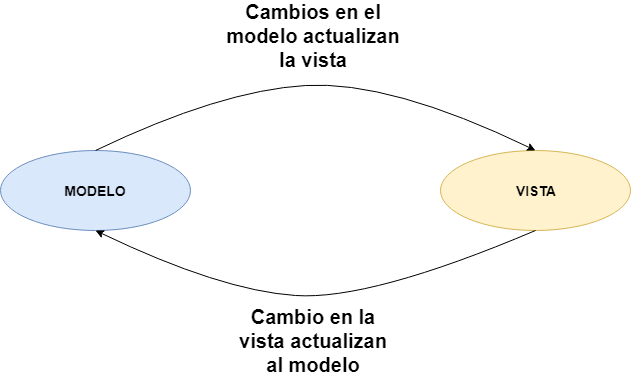
\includegraphics[width=0.6\textwidth, keepaspectratio]{imaxes/MVVM.png}
    \caption{Patrón Modelo-Vista-Vista-Modelo}
    \label{fig:mvvm}
\end{figure}


\subsubsection{Angular~\cite{angular}}
Es un \textit{framework} de desarrollo \textit{Javascript} , creado por Google. Dicho \textit{framework} nos ayuda al desarrollo de aplicaciones web SPA (\textit{Single Page Aplication}).

Se ha decidido utilizar \textit{Angular} por las siguientes razones:
\begin{itemize}
    \item Permite crear aplicaciones modulares y con componentes que pueden ser reutilizables a lo largo de la aplicación, lo que genera un código más limpio y fácil de mantener.
    \item Se integra con bien con \textit{Ionic} para crear aplicaciones híbridas.
    \item Utiliza inyección de dependencias, un patrón que permite instanciar los servicios directamente sin necesidad de crearlos localmente.
    \item Proporciona un programa de línea de comandos que permite generar plantillas para ciertos componentes del código.
    \item Proporciona un conjunto de librerías que facilitan aspectos como la realización de peticiones y envío de datos a través de \textit{HTTP} o navegación entre las páginas de la aplicación.
\end{itemize}

\subsubsection{Ionic~\cite{ionic}}
Es una librería \textit{Javscript} que nos permite construir de manera sencilla y rápida la interfaz de nuestra aplicación.

Se ha decidido usar \textit{Ionic} por las siguientes razones:
\begin{itemize}
    \item Abstrae al diseñador de dibujar los componentes, centrándose en cómo se verán la pantalla.
    \item Permite utilizar la misma interfaz en distintas plataformas, adaptándose automáticamente a estas plataformas (Android, escritorio, web e IOS)
    \item Se integra perfectamente con los \textit{frameworks} más usados del mercado como \textit{Angular}.
    \item Está implementado en su totalidad con componentes web\footnote{Componentes reutilizables que siguen las especificaciones \textit{HTML} y \textit{DOM} establecidas por el \textit{W3C}}, lo que proporciona un rendimiento y compatibilidad mayores.
\end{itemize}

\subsubsection{Capacitor~\cite{capacitor}}
Es una librería \textit{Javascript}, creada por \textit{Ionic}, que contiene una conjunto de herramientas, las cuales nos permiten exportar una aplicación web a una aplicación móvil de manera nativa.

Se ha decidido usar \textit{Capacitor} por las siguientes razones:
\begin{itemize}
    \item Proporciona un desarrollo único para las diferentes plataformas móviles.
    \item Proporciona acceso a los componentes del dispositivo de forma nativa.
    \item Soporte para \textit{plugins} que permiten acceder a nuevas funcionalidades del sistema.
    \item Permite la ejecución de código nativo dentro de la plataforma.

\end{itemize}

\subsubsection{Cypress~\cite{cypress}}

Es un librería \textit{Javascript} que nos permite ejecutar pruebas en aplicaciones web de manera automática, pero pensada para aplicaciones web, ya que dichas pruebas se ejecutan en el navegador y comprueban tanto el correcto funcionamiento de la aplicación como su flujo de ventanas. 

Las ventajas que proporciona \textit{cypress} frente a otras herramientas de pruebas son las siguientes:
\begin{itemize}
    \item Contiene un entorno gráfico que permite una programación más ágil.
    \item Soporta la ejecución de pruebas en cualquier navegador, independientemente del sistema operativo utilizado.
    \item Permite acceder a los elementos que se necesitan probar de una manera sencilla.
\end{itemize}



\subsection{Capa de Negocio}

La capa de lógica de negocio es ejecuta en \textit{NodeJS} y programada en \textit{Typescript} usando para ello el \textit{framework} \textit{NestJS} y otras librerías como: \textit{JWT}, \textit{bcrypt}, \textit{mongoose}\dots~ para autenticicación y conexiones con los servicios.

Adicionalmente, para el desarrollo numérico/computacional se ha usado \textit{Python} y la librería \textit{Sklearn}. 

Se han creado dos servidores [Figura~\ref{fig:servers_schema}] para comunicar ambos lenguajes de programación, donde el servidor de \textit{Python} solo se comunica con el de \textit{Node}, el cual realiza las conexiones al exterior.

\begin{figure}[h]
    \centering
    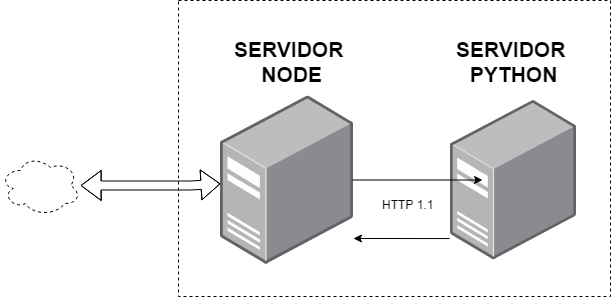
\includegraphics[width=0.6\textwidth, keepaspectratio]{imaxes/servers_schema.png}
    \caption{Capa de lógica de negocio}
    \label{fig:servers_schema}
\end{figure}

\subsubsection{NestJS~\cite{nestjs}}
Es un \textit{framework} de desarrollo para aplicaciones servidor en \textit{NodeJS}. Utiliza Typescript como lenguaje principal de programación y contiene una extensa documentación que abarca la mayor parte de las necesidades requeridas de un servidor.
Las ventajas que proporciona este \textit{framework} son las siguientes:

\begin{itemize}
\item Hace uso de decoradores\footnote{Envolturas que se utilizan sobre funciones, clases\dots~ para añadir más funcionalidad}, lo que supone una programación más ágil, legible y menos propensa a errores.
\item Se integra perfectamente con la mayoría de las herramientas existentes, haciendo que la programación con servicios de terceros funcione correctamente (Base de datos, OpenAPI, Jest~\dots)
\item Utiliza una estructura similar a la usada por \textit{Angular}. Por lo tanto, al usar estos dos \textit{frameworks} en el lado del cliente y el lado del servidor se reduce la complejidad de lectura del código.
\end{itemize}


\subsubsection{Jest~\cite{jest}}

Es un librería \textit{Javascript}, desarrollado por Facebook, que contiene un conjunto de herramientas para ejecutar pruebas de forma automática.

El \textit{framework} de \textit{NestJs} proporciona documentación sobre las pruebas utilizando esta librería, además de ser una de las más usadas en entornos \textit{Javascript}. También proporciona soporte para \textit{Typescript}.

\subsubsection{Sklearn}
\textit{Sklearn}~\cite{sklearn} es una librería de aprendizaje máquina para el lenguaje de programación \textit{Python}.  Se ha usado \textit{Sklearn} por las siguientes razones:
\begin{itemize}
    
\item Se encuentra bien documentada, incluyendo ejemplos para cada función.
\item Mantiene un interfaz consiste ante los distintos modelos de aprendizaje automático.
\item Proporciona funcionalidades adicionales que permiten un desarrollo más ágil.

\end{itemize}

\subsection{Capa de Datos}
Esta capa se encarga de almacenar los datos, para ello se ha usado \textit{MongoDB}, una base de datos NoSQL. Se ha utilizado este tipo de base de datos frente a una relacional por los siguientes motivos:

\begin{itemize}
    \item \textbf{Velocidad:} Debido a que el sistema necesita realizar muchas operaciones de lectura y escritura.
    
    \item \textbf{Volumen:} La aplicación generará una gran cantidad de datos, puesto que estará almacenando principalmente los eventos de un usuario. El volumen de eventos generados de un uso continuado será elevado, por lo que se necesita una base de datos que soporte tal volumen de información.

    \item \textbf{Variabilidad:} La aplicación manejara datos, que pueden no ser consistentes e incluso algunos de ellos pueden modificarse con el tiempo. Este tipo de base de datos no necesitan un esquema para trabajar por lo que las hace ideales para este tipo de casos.

\end{itemize}

\subsubsection{MongoDB~\cite{mongo}}

Es una base de datos orientada a documentos. Los datos están almacenados en documentos JSON y agrupados en colecciones. El formato interno que maneja es BSON, el cual extiende las características de JSON.


Dado que estamos usando una base de datos basada en documentos, el esquema definido para guardar los datos no estará restringido, es decir, se podrán insertar datos no definidos en el esquema. Se ha hecho de esta manera para permitir cambiar el esquema en un futuro, debido a que los datos que se van a guardar pueden ser modificados en el tiempo dado la naturaleza del proyecto.

La base de datos contiene un esquema [Tabla~\ref{tab:mongo_db}] para almacenar los datos de los eventos y por cada tipo de evento se crea un colección.


\begin{table}[h]
    \centering
\begin{tabular}{ c  c}
    \toprule
    \multicolumn{2}{c}{\textbf{EVENTS}} \\
    \midrule
         email      &  String \\
         events     & Object \\
     \bottomrule
\end{tabular}
\caption{Esquema de la base de datos}
    \label{tab:mongo_db}
\end{table}

\section{Herramientas de Gestión y Desarrollo}

Para desarrollar todo este sistema se han utilizado las siguientes herramientas tanto para gestión del proyecto como para el desarrollo del mismo.
\begin{itemize}
    \item \textbf{Git~\cite{git}}: Herramienta para la gestión y control de versiones, desarrollado por Linus Torvalds.
    
    \item \textbf{VS Code~\cite{code}}: \textit{IDE} creado por \textit{Microsoft}, para el desarrollo de software, centrado en lenguaje \textit{Javscript}.
    
    \item \textbf{Android Studio~\cite{android_studio}}: \textit{IDE} creado por \textit{Google}, para el desarrollo de aplicaciones Android.
    
    \item \textbf{Javascript~\cite{javascript}}: Lenguaje de programación creado en 1995 por \textit{Netscape} y \textit{Mozilla}, que sigue el estándar definido por \textit{ECMA}.
    
    \item \textbf{Typescript~\cite{typescript}}: Lenguaje de programación creado por \textit{Microsoft} que es un \textit{superset} de \textit{Javascript}, que esencialmente añade tipos, clases y decoradores.
    
    \item \textbf{Python~\cite{python}}: Lenguaje de programación orientado a objetos, creado por Guido van Rossum en 1991. 
    
    \item \textbf{LaTeX~\cite{latex}}: es un sistema de composición de textos, orientado a la creación de documentos escritos que presenten una alta calidad tipográfica.
    
    
\end{itemize}

 \chapter{Metodología}
\label{chap:metodologia}

En este capítulo se detallarán el conjunto de procedimientos utilizados para alcanzar los objetivos del proyecto.


\section{Desarrollo  incremental}
Este método consiste en una serie de iteraciones, en pequeñas ventanas de tiempo, en las que al final de las mismas tendremos un producto que el cliente podrá revisar y posteriormente mejorar y/o corregir [Figura~\ref{fig:metodologia}]. 

\begin{figure}[h]
    \centering
    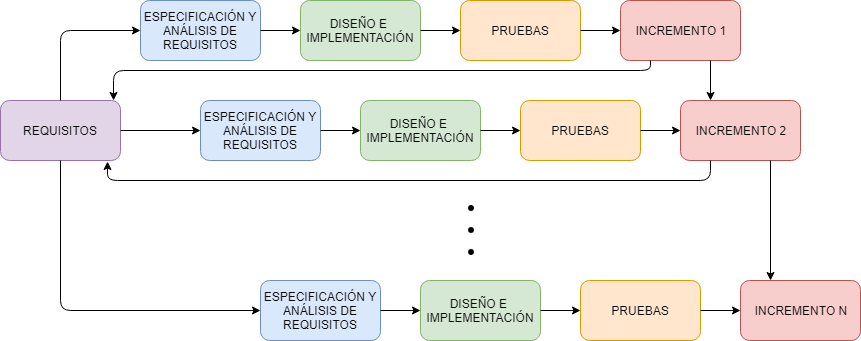
\includegraphics[width=0.8\textwidth, keepaspectratio]{imaxes/Metodologia.png}
    \caption{Fases del modelo incremental}
    \label{fig:metodologia}
\end{figure}

Esta metodología exige tener dos grupos de usuarios:
\begin{itemize}
    \item \textbf{Cliente}: Se encarga de revisar el producto al final de las iteraciones.
    \item \textbf{Desarrollador}: Se encarga de desarrollar el producto.
\end{itemize}

Al ser un proyecto de fin de carrera, no existe un cliente como tal, por lo que se ha decidido que los directores del proyecto tomen el rol de clientes.

Las principales razones por la se ha elegido esta metodología frente a otras existentes son las siguientes:
\begin{enumerate}
    \item \textbf{El cliente no sabe exactamente lo que necesita}: Al inicio del proyecto no se podía prever cómo sería la aplicación, pues debido a la complejidad del proyecto, no se sabía cuál podría ser la mejor manera de hacer que la aplicación para recoger los datos necesarios. 
    
    \item \textbf{Obtener un producto usable rápidamente}: Este proyecto tiene dos etapas claramente diferenciadas, construir una aplicación para recoger datos y analizar esos datos. Claramente la segunda es totalmente dependiente de la primera, por lo que era necesario disponer de un producto usable que permita recopilar información a medida que se amplia su funcionalidad.
    
\end{enumerate}

\section{Iteración 0: Búsqueda de información sobre el dominio}
El objetivo de esta iteración es la búsqueda y recopilación de información sobre el dominio del proyecto. También se definirán los requisitos que el sistema final deberá cumplir, la estructura que se usará para el desarrollo~[Figura~\ref{fig:arquitectura}] y se detallarán los componentes de más bajo nivel~[Figura~\ref{fig:app_schema}]~[Figura~\ref{fig:server_schema}].
De esta forma el desarrollo del proyecto estará bien definido y su implementación debería ser más fácil.

\section{Iteración 1: Sistema de captura de información}
El objetivo de esta fase es la de crear una aplicación que permita capturar la información proveniente del dispositivo. El producto creado al final de esta iteración será una aplicación funcional. El manual de usuario asociado a la aplicación puede consultarse en el Apéndice~\ref{chap:application}.

\subsection{Especificación y análisis de requisitos}
A continuación, se describen los requisitos que la aplicación ha de cumplir:
\begin{itemize}
    \item \textbf{Gestión de los recursos:} Dado que la aplicación recolectará toda la información de los eventos generados por la interacción del usuario con el dispositivo, hay que tener en cuenta cómo manejar dicho volumen de información para evitar el colapso del dispositivo, ya que al tratarse de un \textit{smartphone} o \textit{Tablet}, cuentan con unos recursos limitados tanto en hardware como batería. 
    
     \item \textbf{Formato de los eventos:} Para facilitar el análisis a posteriori la aplicación debe mantener un formato similar en todos los eventos que capture.
     
\end{itemize}


\subsection{Diseño e implementación}
Para realizar la implementación y el diseño de la aplicación se ha usado \textit{Angular} e \textit{Ionic} respectivamente, usando la estructura que se muestra en la Figura~\ref{fig:app_schema}.
 \begin{figure}[h]
    \centering
    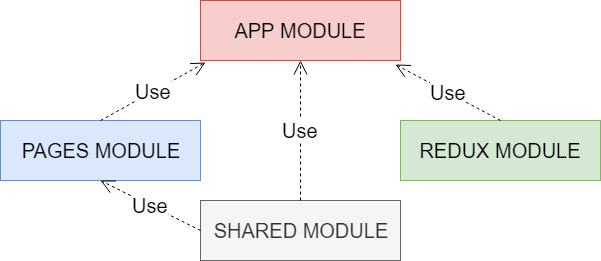
\includegraphics[width=0.8\textwidth, keepaspectratio]{imaxes/APP_SCHEMA.png}
    \caption{Estructura de la aplicación}
    \label{fig:app_schema}
\end{figure}
 
 \subsubsection{App Module}
 Es el módulo principal de la aplicación, en él se encuentra la configuración de los sistemas, y se encarga de hacer de nodo de enlace entre los demás módulos.
 
 
 \subsubsection{Redux Module}
Este módulo implementa toda la lógica del patrón \textit{Redux}. Este patrón permite manejar el estado de la toda aplicación haciendo uso de un objeto central inmutable. Esto permite generar un flujo de datos de una sola dirección y de esta manera que el código sea menos propenso a errores.
 
  \begin{figure}[h]
    \centering
    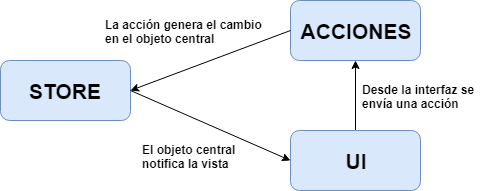
\includegraphics[width=0.8\textwidth, keepaspectratio]{imaxes/redux_simple.png}
    \caption{Ciclo del patrón redux}
    \label{fig:redux_simple}
\end{figure}
 
 \subsubsection{Pages Module}
 Este módulo agrupa al conjunto de ventanas de la aplicación. Cada una de ellas esta implementada en un submódulo. Dicha estructura es implementada por defecto por \textit{Ionic} para poder aplicar la estrategia de carga perezosa (\textit{lazy loading}), la cual solo carga lo que se ve en el momento. Esto permite que la primera carga sea mucho más rápida.
 
 \subsubsection{Shared Module}
 Este módulo contiene los distintos servicios, componentes\dots~ que son reutilizados por varios módulos de la aplicación.
 

\section{Iteración 2: Sistema para el almacenamiento de la información}
En esta fase se pretende crear un servidor que permita el almacenamiento de los eventos recogidos en la primera fase para su posterior análisis. El producto creado al final de esta iteración expone una \textit{API} que se puede consultar en el Apéndice~\ref{chap:rest_api}.

\subsection{Especificación y análisis de requisitos}
A continuación, se describen los requisitos que el servidor ha de cumplir:
\begin{itemize}
    \item \textbf{Gestión de los recursos:} Dado que el servidor ha de permitir el envío y recibo de muchas peticiones por segundo, se ha de tener en cuenta, que el servidor soporte dicha funcionalidad a un coste de recursos bajo.
    
     \item \textbf{Almacenamiento de los eventos:} Dado que la cantidad de eventos que se manejarán será muy alta y con un esquema semi-definido, ya que podría cambiar en un futuro, se necesita una base de datos que sea compatible con estos puntos.
\end{itemize}
\subsection{Diseño e implementación}
 Debido a los requisitos comentados se ha optado por usar Node.js como entorno, por su bajo consumo de recursos. La estructura generada se puede ver en la Figura~\ref{fig:server_schema}.
 
 \begin{figure}[h]
    \centering
    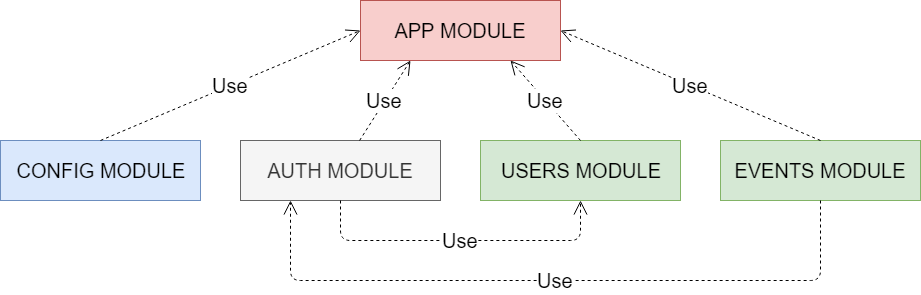
\includegraphics[width=0.8\textwidth, keepaspectratio]{imaxes/server_schema.png}
    \caption{Estructura de la aplicación}
    \label{fig:server_schema}
\end{figure}
 
 \subsubsection{App Module}
 Es el módulo principal desde el cual se llaman a los otros módulos e inicia servicios de terceros, como la conexión con la base datos.
 
 \subsubsection{Config Module}
Este módulo contiene todas las variables externas del sistema, como el puerto, dirección de la base de datos~\dots
 
 \subsubsection{Auth Module}
 En este módulo se realiza la autenticación del usuario, la cual permitirá al usuario realizar ciertas acciones y restringirá otras en función a su rol.
 
  \subsubsection{Users Module}
 En este módulo se encuentra la lógica encargada de procesar la información de los usuarios, como la creación y actualización de estos.
 
 \subsubsection{Events Module}
 En este módulo se encuentra la lógica necesaria para procesar la información relacionada con los eventos que se generan en la aplicación, almacenándolos de forma persistente en la base de datos.

\section{Iteración 3: Comunicar aplicación con servidor}
El objetivo de esta fase es la de comunicar los dos sistemas creados hasta el momento, con el fin de guardar los eventos generados en la primera iteración
      
\subsection{Especificación y análisis de requisitos}
A continuación, se describen los requisitos establecidos para esta iteración:

\begin{itemize}
    \item \textbf{Securizar  conexiones}: Dado que la comunicación se pretende realizar a través de internet usando el protocolo \textit{HTTP 1.1}, es necesario que esta comunicación permanezca cifrado de punto a punto, por lo que usarán los protocolos criptográficos \textit{SSL/TLS}.
    
    \item \textbf{Restringir peticiones}: Algunas peticiones hacia nuestro servidor deberán estar solo disponibles si el usuario cumple ciertas restricciones. Estás peticiones deberán ser realizadas por un usuario administrador.
    
\end{itemize}

\subsection{Diseño e implementación}

Para segurizar toda nuestra aplicación y hacer que esta sea menos propensa a ataques, se ha creado un certificado digital para poder realizar conexiones \textit{HTTPS}.

Para restringir el acceso a nuestro servidor hemos utilizado el estándar \textit{JSON Web Token} (\textit{JWT}), el cual es una cadena de texto codificada que se envía en cada petición. Esta cadena de texto contiene tres partes que contienen la información necesaria para comprobar el usuario y la validez del token.

 \section{Iteración 4: Implementación de la Inteligencia Artificial}
 
 El objetivo de esta iteración es la de tratar los datos obtenidos. Analizando que características obtienen un mejor resultado a la hora de identificar al usuario. Esta iteración se detallará más a fondo en el capítulo \ref{chap:ia}.
 
 \subsection{Especificación y análisis de requisitos}
A continuación, se describen los requisitos establecidos para esta iteración:

\begin{itemize}
    \item \textbf{Obtener un conjunto de datos grande}: Para este tipo de análisis se necesitan  una gran cantidad de datos y representativos de la población. Por lo tanto, es necesario obtener datos de bastantes usuarios de diferentes edades y sexos.
    
    \item \textbf{Obtener características no relacionadas}: Para analizar los eventos, lo ideal es obtener características poco correlacionadas, ya que si estas están correlacionadas estos datos serán redundantes. Es decir, no aportarán ninguna información adicional, pero podrán empeorar los resultados.
\end{itemize}

 \section{Iteración 5: Implementación online de los algoritmos}
 El objetivo de esta iteración es conseguir que el algoritmo entrenado sea accesible en cualquier momento y que su respuesta sea la predicción.
 
 
 \subsection{Especificación y análisis de requisitos}
A continuación, se describen los requisitos establecidos para esta iteración:

\begin{itemize}
    \item \textbf{Integrar los servidores}: Para que el algoritmo no este expuesto directamente en internet, sino que solo sea accesible mediante el servidor principal. De esta manera, la configuración relacionada con la seguridad solo será necesario implementarla en un servidor.
    
    \item \textbf{Gestión de recursos}:  El servidor se encontrará en un maquina física por lo que es necesario controlar que los procedimientos que se lleven a cabo no sean computacionalmente costosos.   
\end{itemize}
 
 \subsection{Diseño e implementación}
 Para conseguir el objetivo de esta iteración se ha creado un servidor en \textit{Python} que permita la ejecución de un conjunto de librerías las cuales usarán el algoritmo entrenado y la respuesta de la petición generada será la predicción hecha por el algoritmo. 

\section{Pruebas}
\label{cap:pruebas}

Las pruebas son las actividades dirigidas a evaluar la capacidad de un programa o sistema y determinar que alcanza los resultados requeridos \cite{hetzel1988complete}.

Existen distintos niveles de pruebas, según se puede observar en la Figura \ref{fig:cohn}, el nivel más bajo pertenecen a las pruebas unitarias, que son las que mayor atención deberemos prestar, seguidas de las pruebas de integración y por último las pruebas \textit{e2e}. 

\begin{figure}[H]
    \centering
    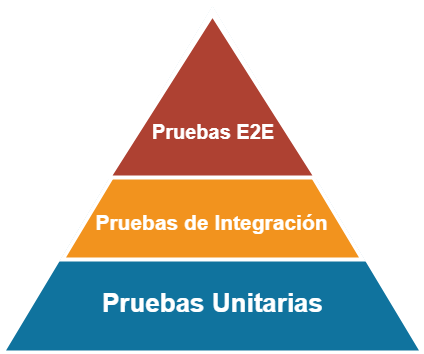
\includegraphics[width=0.5\textwidth]{imaxes/piramide_cohn.png}
    \caption[Pirámide de Cohn]{Pirámide de Cohn \cite{cohn2010succeeding}}
    \label{fig:cohn}
\end{figure}

\subsection{Prueba unitarias}

Estas pruebas son de muy bajo nivel, en ellas se comprueba el correcto funcionamiento de los métodos, clases, componentes\dots

Este tipo de pruebas han sido ejecutadas tanto en el servidor como en la aplicación, para validar el correcto funcionamiento de algunas de las partes más críticas del sistema.

\subsection{Pruebas de integración}

Comprueban el correcto funcionamiento de los componentes una vez integrados. Se ha revisado la integración completa del sistema, validando que todos los módulos funcionasen correctamente.

Este tipo de pruebas han sido ejecutadas en el servidor para validar las rutas creadas. Se han implementado tres bancos de pruebas, cada uno de ellos perteneciente a un módulo de nuestro sistema. En total se han ejecutado doce casos diferentes, y todas han sido satisfactorias [Figura \ref{fig:test_suite_server}]

\begin{figure}[H]
    \centering
    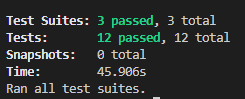
\includegraphics[width=0.5\textwidth]{imaxes/test_suites_server.png}
    \caption{Resultado de las pruebas en el servidor}
    \label{fig:test_suite_server}
\end{figure}

\subsection{Pruebas end to end (e2e)}
Este tipo de pruebas simulan el comportamiento de un usuario real. Prueban toda la aplicación de principio a fin, verificando el correcto funcionamiento de todo el sistema y la navegación entre las distintas ventanas de la aplicación.

\begin{figure}[H]
    \centering
    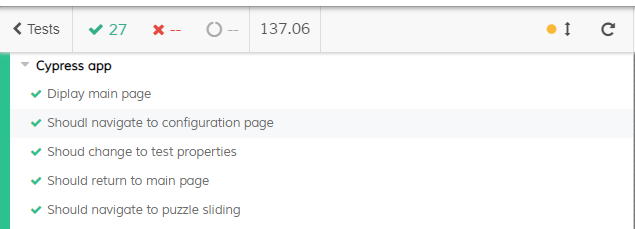
\includegraphics[width=0.7\textwidth]{imaxes/test_suites_app.png}
    \caption[Resultado de las pruebas en la aplicación]{Resultado de las pruebas en la aplicación \cite{cypress_youtube}}
    \label{fig:test_suite_app}
\end{figure}

\subsection{Cobertura}

La cobertura es una medida que nos ayuda a comprobar que partes de nuestro código han sido probadas. Además, sirve para determinar la calidad de la prueba, pues gracias a ella podremos saber que partes del código no hemos comprobado y cuales sí.

\begin{landscape}
    \begin{figure}
        \centering
        
        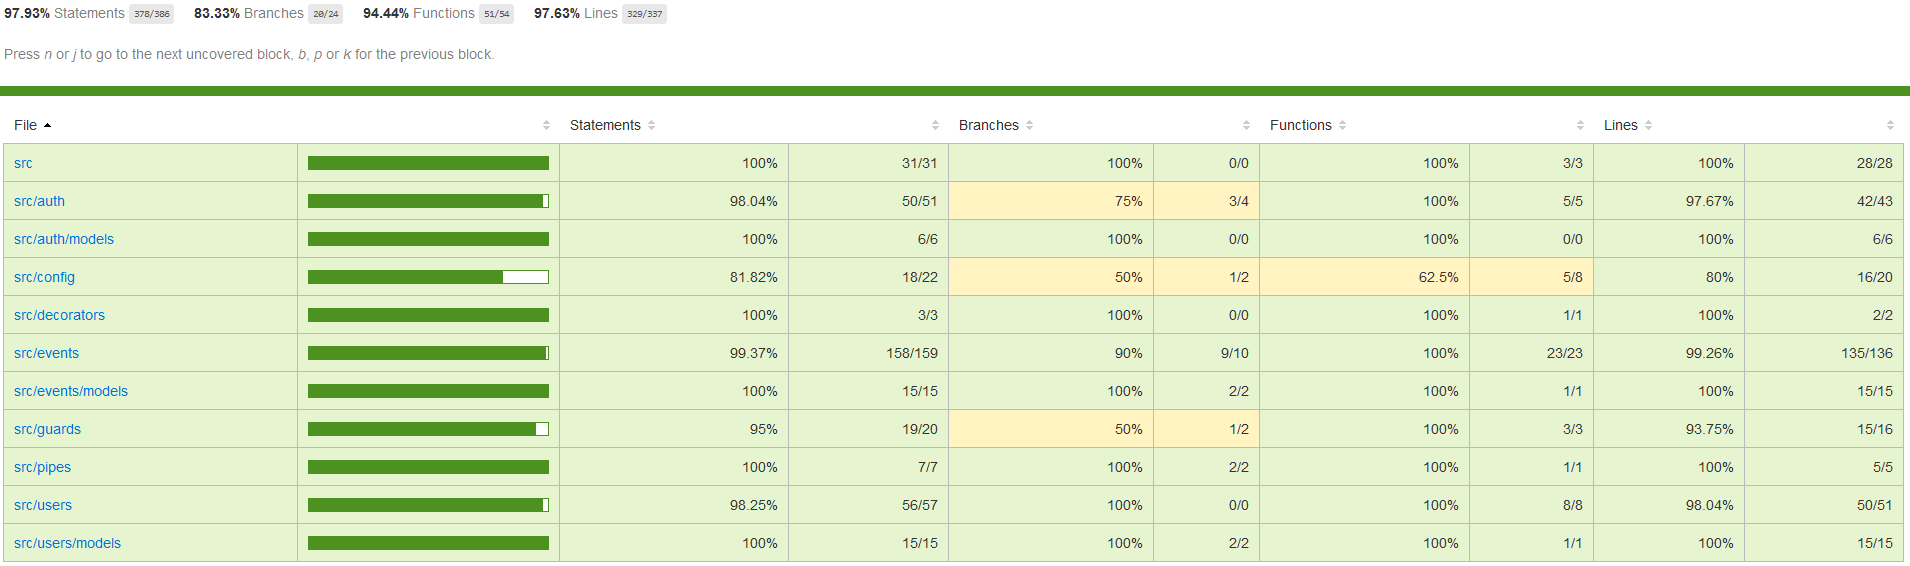
\includegraphics[width=\linewidth,height=0.6\textheight]{imaxes/server_coverage.png}
        \caption{Cobertura de las pruebas del servidor}
        \label{fig:server_coverage}
    \end{figure}
\end{landscape}


 \include{contido/pruebas}
 \chapter{Análisis y tratamiento de datos}
\label{chap:ia}

Para implementar un sistema de Inteligencia Artificial, en adelante \textit{IA}, que clasifique un conjunto de datos, necesitaremos obtener mucha información para \textit{alimentarla}. Estos datos normalmente en bruto contienen información redundante, valores atípicos, campos nulos\dots~ todo esto haría que nuestra \textit{IA} se viese afectada negativamente, para ello necesitaremos tratar correctamente los datos.

En la última parte del capítulo se seguirá el proceso de selección de los algoritmos más plausibles, así como su ajuste para refinar progresivamente los modelos elaborados.

En el Capítulo \ref{chap:resultados}, se mostrarán y analizarán los resultados obtenidos después de realizar el procedimiento mencionado en este capítulo.

\section{Tratamiento de los datos}

La mayoría de los de algoritmos de aprendizaje presentan varias necesidades previas a la hora de trabajar con un conjunto de datos. Por ello, se necesita procesar la información y formatearla correctamente para los entrenamientos. 
En esta sección se abordarán las técnicas empleadas para solventar dicho problema.

\subsection{Variables de texto}

La mayoría de los algoritmos de aprendizaje mejor con números que con etiquetas. Para que nuestros datos se adecuen a estas circunstancias debemos manipularlos correctamente.


Nuestro conjunto de datos solo presenta una variable de texto que es la de usuario, la cual hace referencia al dueño del evento. Para formatear estos valores a números, se ha usado una función de la librería de \textit{Sklearn}, la cual asigna un único valor a cada etiqueta.
 \subsection{Variables categóricas}
 Estas variables representa un conjunto de datos, es decir, cada valor representa una categoría.
 
En nuestro caso el dato dirección es una variable categórica, en la cual cada valor representa una dirección única. Sino formateamos este valor, el algoritmo entenderá que los valores más próximos están más relacionados.
Para solucionar este problema hemos usado una función de la librería de \textit{Sklearn}, la cual genera una columna por cada valor posible y le asigna el valor cero o uno en función del valor de la columna original~[Tabla~\ref{tab:categorical_feature}].

\begin{table}[H]
    \centering
    \begin{tabular}{ c || c c c }
\toprule
\textbf{Columna Original} & \multicolumn{3}{c}{\textbf{Columna Transformada}} \\
\midrule
direction &  direction\_4 &  direction\_8 &  direction\_16 \\
\midrule
8  &             0 &            1 &             0 \\
4  &             1 &            0 &             0 \\
16 &             0 &            0 &             1 \\
\bottomrule
\end{tabular}
    \caption{Corrección de la variable categórica}
    \label{tab:categorical_feature}
\end{table}

\subsection{Valores Nulos}

La mayoría de los algoritmos de aprendizaje no pueden trabajar con valores nulos, por lo tanto, necesitamos tratar nuestros datos para detectarlos y procesarlos correctamente. 
Para realizar este paso se contemplaron las siguientes opciones:

\begin{enumerate}
    \item Eliminar la fila que los contiene.
    \item Eliminar la columna que los contiene.
    \item Rellenar a cero dichos valores.
    \item Rellenar los valores con la mediana.
\end{enumerate}

De las opciones mencionas se eligió la última ya que es menos agresiva a la hora de modificar los datos. La librería de \textit{Sklearn} proporciona un método que nos ayuda con este proceso, y asigna a los valores nulos el valor que hemos escogido, en nuestro caso la mediana.

\subsection{Transformación de las características}

Para encontrar nuevas relaciones entre las características y las clases se ha utilizado el método de \textit{polynomial feature} de la librería \textit{Sklearn}.

En el ejemplo de la Figura~\ref{fig:polynomial} la imagen de la izquierda representa un problema linealmente no separable. Pero si elevamos al cuadrado la características $x_1$ los datos pasan a ser linealmente separables.

\begin{figure}[h]
    \centering
    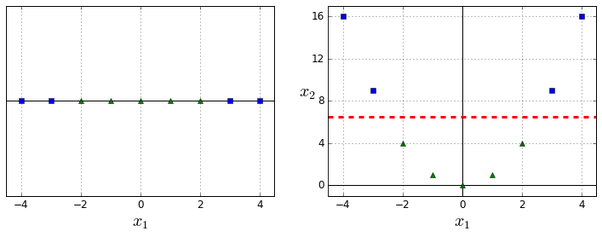
\includegraphics[width=0.8\textwidth, keepaspectratio]{imaxes/polinomial.png}
    \caption{Ejemplo de Polynomial Feature}
    \label{fig:polynomial}
\end{figure}

En este proyecto se utilizo esta técnica para generar características de segundo grado, es decir, si tenemos las características $[a, b]$, el segundo grado sería $[1, a, b, a^2, ab, b^2]$.

\subsection{Estandarizar los datos}
La mayor parte de los algoritmos de aprendizaje disminuyen su rendimiento cuando los valores de las variables se mueven en un rango muy amplio. Dentro de las características de los eventos existen varias variables con esta problemática, como es el caso de \textit{duración}. Esta variable tiene un valor medio de 122 \textit{ms} mientras que su rango de valores es~[13, 1654]~[Tabla~\ref{tab:scaler_example}].

\begin{table}[H]
    \centering
    \begin{tabular}{lrrrrrrrr}
        \toprule
        {} &   count &        mean &        std &   min &   25\% &    50\% &    75\% &     max \\
        \midrule
        duration &  3436.0 &  122.40 &  72.48 &  13.0 &  83.0 &  104.0 &  146.0 &  1654.0 \\
        \bottomrule
    \end{tabular}
    \caption{Estadísticas de la característica duración}
    \label{tab:scaler_example}
 \end{table}
 
 Para realizar esta tarea se hace uso de la librería \textit{Sklearn}, la función utilizada realiza el siguiente proceso:
\begin{itemize}
\item Resta el valor medio, lo cual hace que los valores cerca de la media tiendan a cero.
\item Divide el valor por el rango intercuartílico~\footnote{Diferencia entre el tercer y el primer cuartil}. Se usan los cuartiles como valor de división porque hace que sea menos propenso a los valores atípicos
\end{itemize}

\section{Selección de algoritmos}

Para realizar las pruebas iniciales se han seleccionado los siguientes algoritmos:

\begin{itemize}
    \item \textbf{LogisticRegression (LR)}~(Véase Sección~[\ref{sec:logistic_regresion})
    
    \item \textbf{RandomForest (RF)}~(Véase Sección~\ref{sec:random_forest})
    
    \item \textbf{DecisionTree (DT)}~(Véase Sección~\ref{sec:decision_tree})
    
    \item \textbf{Perceptrón Multicapa (MLP)}~(Véase Sección~\ref{sec:mlp})
    
    \item \textbf{K-Nearest Neighbors (kNN)}~(Véase Sección~\ref{sec:kn})
    
    \item \textbf{Máquinas de soporte vectorial (SVM)}~(Véase Sección~\ref{sec:svm})
\end{itemize}

El primer paso consiste en realizar una prueba para tener un punto de inicio sobre el cuál comparar los resultados, y de esta manera comprobar analíticamente si las técnicas aplicadas a lo largo del capítulo han servido para mejorar la clasificación.

Analizando los resultados de la Tabla~\ref{table:clf_alg} en general todos los algoritmos obtienen unos valores similares en las columnas de \textit{Recall}, \textit{Precision} y \textit{F1 Score}, con una desviación del ±5\%. Si comparamos los resultados de los algoritmos individualmente podemos obtener las siguientes conclusiones:

\begin{itemize}
    \item \textbf{\textit{RF}}: Los resultados obtenidos por este algoritmo en la columna de \textit{precision} son los más altos exceptuando el evento de \textit{tap}. Los tiempos de entrenamiento (\textit{Fit Time}) están muy por debajo del resto de algoritmos.

    \item \textbf{\textit{DT}}: Los valores de las columnas de \textit{Recall}, \textit{Precision} y \textit{F1 Score} se mantienen en un rango de valores pequeño. 

    \item \textbf{\textit{LR}}: Los valores obtenidos en la columna \textit{precision} son los segundos más altos excepto en \textit{tap} donde es el más alto y, al igual que \textit{RF} el tiempo de entrenamiento suele ser bajo.
    
    \item \textbf{\textit{MLP}}: Los tiempos de predicción (\textit{Score Time}) obtenidos son los más bajos en todos los eventos.

    \item \textbf{\textit{SVM}}: Su desviación es la más alta y, por lo tanto, optimizando sus parámetros podría reducirse esta desviación y mejorando los resultados.

    \item \textbf{\textit{kNN}}: Este algoritmo obtuvo el rendimiento más bajo tanto en \textit{precision} como en \textit{Fit Time}.
\end{itemize}

Para reducir el tiempo de procesamiento y optimizar la búsqueda se ha decidido los siguientes algoritmos:
\begin{itemize}
    \item (\textit{DT}) debido a que \textit{RF} obtiene mejores resultados y al ser este un conjunto de \textit{DT} es redundante entrenar dos algoritmos de características similares. 
    \item \textit{KN} porque sus valores son lo que han obtenido el rendimiento más bajo.
\end{itemize}



\begin{table}[!h]
\centering
\begin{tabular}{ c l c c c c c }
\toprule
Evento & Alg. &  Recall & Precision & F1 Score & \thead{Fit \\ Time (s)} & \thead{Score \\ Time (s)} \\
\midrule
\multirow{6}{*}{\rotatebox[origin=c]{90}{motion}} &  \textit{DT} &  71.01\% (±0.122) &  71.96\% (±0.10 8) &  71.11\% (±0.110) &  0.072 &  0.121 \\
& \textit{kNN} &  70.85\% (±0.122) &  70.48\% (±0.108) &  70.29\% (±0.110) &  0.225 &  0.125 \\
& \textit{LR} &  71.22\% (±0.130) &  73.14\% (±0.112) &  71.76\% (±0.115) &  0.088 &  0.182 \\
& \textit{MLP} &  71.66\% (±0.120) &  71.48\% (±0.107) &  71.22\% (±0.107) &  0.269 &  0.094 \\
& \textit{RF} &  71.09\% (±0.135) &  76.33\% (±0.104) &  73.33\% (±0.118) &  0.054 &  0.324 \\
& \textit{SVM} &  69.01\% (±0.139) &  70.82\% (±0.123) &  69.08\% (±0.118) &  0.193 &  0.118 \\
\midrule
\multirow{6}{*}{\rotatebox[origin=c]{90}{multitouch}}  &  \textit{DT} &  71.45\% (±0.126) &  72.55\% (±0.110) &  71.58\% (±0.112) &  0.073 &  0.145 \\
 & \textit{kNN} &  70.98\% (±0.120) &  70.82\% (±0.107) &  70.51\% (±0.108) &  0.251 &  0.103 \\
 & \textit{LR} &  71.70\% (±0.131) &  74.40\% (±0.108) &  72.55\% (±0.113) &  0.044 &  0.246 \\
 & \textit{MLP} &  71.61\% (±0.121) &  71.75\% (±0.108) &  71.30\% (±0.108) &  0.147 &  0.105 \\
 & \textit{RF} &  75.95\% (±0.120) &  77.86\% (±0.097) &  76.52\% (±0.104) &  0.048 &  0.326 \\
 & \textit{SVM} &  69.74\% (±0.138) &  71.00\% (±0.119) &  69.53\% (±0.115) &  0.206 &  0.122 \\
\midrule
\multirow{6}{*}{\rotatebox[origin=c]{90}{orientation}} &  \textit{DT}  &  71.86\% (±0.121) &  72.82\% (±0.106) &  71.95\% (±0.108) &  0.071 &  0.128 \\
 & \textit{kNN}&  71.37\% (±0.120) &  71.01\% (±0.106) &  70.81\% (±0.107) &  0.233 &  0.118 \\
 & \textit{LR}&  72.25\% (±0.130) &  74.53\% (±0.107) &  72.95\% (±0.112) &  0.072 &  0.199 \\
 & \textit{MLP}&  72.13\% (±0.119) &  72.02\% (±0.105) &  71.72\% (±0.106) &  0.220 &  0.097 \\
 & \textit{RF}&  75.41\% (±0.110) &  79.54\% (±0.086) &  77.14\% (±0.096) &  0.053 &  0.325 \\
 &\textit{SVM} &  69.51\% (±0.138) &  71.38\% (±0.119) &  69.61\% (±0.115) &  0.196 &  0.119 \\
\midrule
\multirow{6}{*}{\rotatebox[origin=c]{90}{pan}} &   \textit{DT} &  70.96\% (±0.122) &  71.71\% (±0.110) &  70.97\% (±0.110) &  0.069 &  0.115 \\
& \textit{kNN}&  70.65\% (±0.129) &  70.06\% (±0.111) &  69.93\% (±0.113) &  0.218 &  0.128 \\
& \textit{LR}&  70.59\% (±0.129) &  72.38\% (±0.113) &  71.05\% (±0.115) &  0.084 &  0.168 \\
& \textit{MLP}&  71.19\% (±0.122) &  71.11\% (±0.108) &  70.75\% (±0.110) &  0.271 &  0.090 \\
& \textit{RF}&  70.29\% (±0.133) &  75.78\% (±0.110) &  72.60\% (±0.121) &  0.053 &  0.324 \\
&\textit{SVM} &  67.57\% (±0.162) &  71.14\% (±0.125) &  67.91\% (±0.137) &  0.188 &  0.115 \\
\midrule
\multirow{6}{*}{\rotatebox[origin=c]{90}{swipe}} &  \textit{DT}  &  72.07\% (±0.125) &  73.09\% (±0.109) &  72.17\% (±0.111) &  0.070 &  0.136 \\
&\textit{kNN}&  71.42\% (±0.120) &  71.18\% (±0.107) &  70.92\% (±0.108) &  0.242 &  0.111 \\
&\textit{LR}&  73.25\% (±0.132) &  75.39\% (±0.106) &  73.87\% (±0.113) &  0.044 &  0.220 \\
&\textit{MLP}&  72.20\% (±0.121) &  72.13\% (±0.106) &  71.80\% (±0.108) &  0.158 &  0.101 \\
&\textit{RF}&  77.98\% (±0.104) &  80.90\% (±0.091) &  79.13\% (±0.094) &  0.049 &  0.326 \\
&\textit{SVM}&  69.97\% (±0.137) &  71.44\% (±0.120) &  69.88\% (±0.115) &  0.201 &  0.120 \\
\midrule
\multirow{6}{*}{\rotatebox[origin=c]{90}{tap}} &   \textit{DT} &  70.55\% (±0.125) &  72.10\% (±0.111) &  70.92\% (±0.112) &  0.078 &  0.156 \\
& \textit{kNN} &  71.17\% (±0.120) &  71.11\% (±0.106) &  70.76\% (±0.108) &  0.261 &  0.098 \\
& \textit{LR} &  70.15\% (±0.125) &  74.98\% (±0.108) &  72.15\% (±0.114) &  0.046 &  0.280 \\
& \textit{MLP} &  71.03\% (±0.119) &  71.74\% (±0.109) &  71.03\% (±0.108) &  0.140 &  0.110 \\
& \textit{RF}  &  68.49\% (±0.072) &  73.82\% (±0.082) &  70.98\% (±0.075) &  0.048 &  0.327 \\
& \textit{SVM} &  70.72\% (±0.128) &  70.15\% (±0.111) &  70.00\% (±0.112) &  0.212 &  0.125 \\
\bottomrule
\end{tabular}

\caption{Resultados de la primera ejecución}
\label{table:clf_alg}
\end{table}

\newpage

\section{Selección de hiperparámetros }

En esta sección se verá cómo se han configurado los algoritmos. Dicha configuración se materializa a través de los hiperparámetros. Estos son valores que se establecen antes del entrenamiento del algoritmo y que deciden en parte como van a funcionar dichos algoritmos, permitiendo que se ajusten mejor al modelo.

Para buscar estos hiperparámetros  Se suelen utilizar dos técnicas:
\begin{itemize}
    \item \textbf{\textit{Grid Seach}}: Es un busca exhaustiva de los mejores parámetros sobre una combinación dada.
    \item \textbf{\textit{Random Search}}: Es un búsqueda aleatoria sobre una combinación de parámetros dada.
\end{itemize}

Para este proyecto se ha usado la técnica de \textit{Grid Search} como la idónea debido a publicaciones~\cite{bergstra2012random} sobre el rendimiento de ambas técnicas. 

Para analizar los resultados y obtener un valor los más aproximado posible se han seguido los siguientes pasos:
\begin{enumerate}
    \item Se han ordenado los resultados en orden descendente y se han seleccionado los cinco mejores valores de cada algoritmo.
    \item Se han calculado las puntuaciones medias de esos valores y su desviación, con el fin de obtener unos tiempos y puntuaciones medios [Tabla \ref{tab:mean_hyper_values}] para los mejores hiperparámetros.
    \item Se han calculado también los valores más comunes para obtener los mejores hiperparámetros  [Tabla \ref{tab:searched_hyper}].
\end{enumerate}


\begin{table}[!h]
    \centering
\begin{tabular}{c l c c c }
\toprule
Evento & Alg. &   Precision & Fit Time (s) & Score Time (s) \\
\midrule
\multirow{4}{*}{\rotatebox[origin=c]{90}{motion} }
&  \textit{LR}    &   63.23\% (± 0.047) & 1.1629 (± 0.047)  &   0.0268 (± 0.047)\\
& \textit{MLP}   &   65.79\% (± 0.080) & 10.4182 (± 0.080) &   0.0923 (± 0.080)\\
& \textit{RF}    &   68.42\% (± 0.060) & 0.3167 (± 0.060)  &   0.0160 (± 0.060)\\
& \textit{SVM}   &   65.64\% (± 0.132) & 0.1740 (± 0.132)  &   0.0762 (± 0.132)\\
\midrule

\multirow{4}{*}{\rotatebox[origin=c]{90}{multitouch} }
& \textit{LR}   &    76.98\% (± 0.128) & 0.0346 (± 0.128) &  0.0164 (± 0.128)\\
& \textit{MLP}  &    80.99\% (± 0.030) & 0.6049 (± 0.030) &  0.0218 (± 0.030)\\
& \textit{RF}   &    86.93\% (± 0.089) & 0.0811 (± 0.089) &  0.0091 (± 0.089)\\
& \textit{SVM}  &   100.00\% (± 0.000) & 0.0059 (± 0.000) &  0.0043 (± 0.000) \\
\midrule

\multirow{4}{*}{\rotatebox[origin=c]{90}{orienntation} }
& \textit{LR}   &    70.09\% (± 0.069) & 12.5253 (± 0.069) &  0.0248 (± 0.069)\\
& \textit{MLP}  &    66.72\% (± 0.033) & 28.8783 (± 0.033) &  0.1177 (± 0.033)\\
& \textit{RF}   &   77.28\% (± 0.048) & 0.1783 (± 0.048) &   0.0133 (± 0.048)\\
& \textit{SVM}  &   90.43\% (± 0.152) & 0.1458 (± 0.152) &   0.0746 (± 0.152)\\
\midrule

\multirow{4}{*}{\rotatebox[origin=c]{90}{pan} }
& \textit{LR}   & 67.48\% (± 0.148) & 0.1268 (± 0.148) &     0.0103 (± 0.148)\\
& \textit{MLP}  & 77.65\% (± 0.089) & 1.1181 (± 0.089) &     0.0334 (± 0.089)\\
& \textit{RF}   & 80.99\% (± 0.094) & 0.1343 (± 0.094) &     0.0122 (± 0.094)\\
& \textit{SVM}  & 78.96\% (± 0.099) & 0.0067 (± 0.099) &     0.0045 (± 0.099)\\
\midrule

\multirow{4}{*}{\rotatebox[origin=c]{90}{swipe} }
& \textit{LR}   &  84.67\% (± 0.043) & 0.5641 (± 0.043) &    0.0241 (± 0.043)\\
& \textit{MLP}  &  81.14\% (± 0.044) & 0.7857 (± 0.044) &    0.0822 (± 0.044)\\
& \textit{RF}   &  85.56\% (± 0.045) & 0.1575 (± 0.045) &    0.0130 (± 0.045)\\
& \textit{SVM}  &  94.07\% (± 0.066) & 0.0847 (± 0.066) &    0.0383 (± 0.066)\\
\midrule
\multirow{4}{*}{\rotatebox[origin=c]{90}{tap}}
& \textit{LR}    & 70.54\% (± 0.080) & 0.1695 (± 0.080) &     0.0149 (± 0.080)\\
& \textit{MLP}   & 75.42\% (± 0.090) & 7.6387 (± 0.090) &     0.1006 (± 0.090)\\
& \textit{RF}    & 75.52\% (± 0.092) & 0.1926 (± 0.092) &     0.0149 (± 0.092)\\
& \textit{SVM}   & 85.90\% (± 0.100) & 0.0768 (± 0.100) &     0.0278 (± 0.100)\\
\bottomrule
\end{tabular}
\caption{Resultados medios con los mejores hiperparámetros }
    \label{tab:mean_hyper_values}
\end{table}


\begin{table}[H]
    \centering
    \begin{tabular}{ c c c c }
        \toprule
        \multicolumn{4}{c}{\textbf{Random Forest}} \\
        \midrule
        Criterion &  Max Depth  & Max Features     &  Number Of Estimators \\
        \midrule
        gini    &   5.0        &   log2            & 21.0 \\
        \bottomrule
        \multicolumn{4}{c}{\textbf{Support Vector Machines}} \\
        \midrule
        Gamma     & C            & \multicolumn{2}{c}{Kernel}\\
        \midrule
        0.1       &  1.0         & \multicolumn{2}{c}{rbf}  \\
        \midrule
        \multicolumn{4}{c}{\textbf{Multilayer Perceptron}} \\
        \midrule
        Solver    &  Alpha       &  \multicolumn{2}{c}{Hidden Layer Sizes}  \\
        \midrule
        lbfgs     &  10.0        & \multicolumn{2}{c}{60.0}   \\
        \bottomrule
    \end{tabular}
    \caption{Mejores hiperparámetros  para cada algoritmo}
    \label{tab:searched_hyper}
\end{table}

\newpage


\section{Selección de características}
\label{sec:sel_cara}
En esta sección se detallarán las técnicas utilizadas para la selección de características y los resultados obtenidos. La selección de características es una técnica que permite distinguir qué características son las más importantes a la hora de clasificar nuestros datos, esta técnica aporta las siguientes mejoras:

\begin{enumerate}
    \item A menudo aumenta la precisión de la clasificación a través de la eliminación de características irrelevantes, redundantes o altamente correlacionadas.
    \item Eliminar características redundantes implica que exista un menor riesgo de \textit{overfitting}.
    \item Disminuye la cantidad de características, lo que hace que el proceso de entrenamiento del modelo sea más eficiente
\end{enumerate}

Existen diferentes técnicas para la selección de características, algunas de ellas son:

\begin{itemize}
    \item \textbf{Selección univariante}: Muestra la relación de la salida con las variables  de entrada basándose en métodos estadísticos, como chi cuadrado.
    \item \textbf{\textit{Recursive feature elimination} (RFE)}: Esta técnica consiste en ir eliminar progresivamente las características menos relevantes.
    \item \textbf{Basada en árboles}: Esta técnica consiste en entrenar un algoritmo basado en árboles, como el \textit{Random Forest}, y después examinar que características son más relevantes para el algoritmo.
\end{itemize}

Para seleccionar las características hemos empleado el último método~[Figura~\ref{fig:origianlvsselected}]. 
Se ha descartado aplicar la primera técnica porque solo es confiable si las características son completamente independientes. La segunda técnica fue descartada porque los algoritmos \textit{SVM}, con un kernel no lineal, y \textit{MLP} no exponen los coeficientes con los pesos internos de las características necesarios para aplicar \textit{RFE}. 

\begin{figure}[h]
\centering
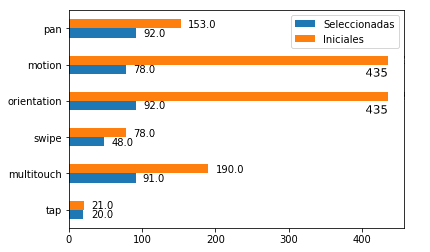
\includegraphics[width=0.8\textwidth]{imaxes/plots/selectedvsoriginal_features.png}
\caption{Características Iniciales VS Características Seleccionadas}
\label{fig:origianlvsselected}
\end{figure}



 \chapter{Resultados}
\label{chap:resultados}

En este capítulo se presentarán los resultados obtenidos para cada una de las técnicas exploradas. Para ello se utilizarán las métricas de \textit{precision}, \textit{acuraccy}, \textit{F1 Score}, \textit{Fit Time} y \textit{Score Time} (véase la Sección~\ref{sec:metrics}) y los algoritmos \textit{Random Forest}, \textit{SVM}, \textit{MLP} y votación.

Dada la gran cantidad de conjuntos de entrenamiento que se han establecido, primero se analizarán los resultados globales agrupados por eventos y, posteriormente, se expandirán para cada uno de los usuarios. Por último, se mostrarán los resultados obtenidos de la prueba online.


\section{Datos agrupados por eventos}
En esta sección se presenta el rendimiento que han ofrecido los diferentes algoritmos. En la Tabla~\ref{tab:final_results_all_features} se muestran los resultados obtenidos utilizando todas las características de los eventos.

\begin{table}[!h]
    \centering
    \begin{tabular}{l l c c c c c c}
\toprule
Ev. & Alg. & \thead{Accuracy \\ (\%)} & \thead{Precision \\ (\%)} & \thead{Recall \\ (\%)} & \thead{F1 Score \\ (\%)} & \thead{Fit \\ Time(s)} & \thead{Score \\ Time(s)} \\
\midrule
\multirow{4}{*}{\rotatebox{90}{tap}} 
&         Vot.  & 74.66\ {\footnotesize  (±0.05)} &  77.08\ {\footnotesize  (±0.07)} &  73.52\ {\footnotesize  (±0.09)} &  74.82\ {\footnotesize  (±0.06)} & 0.197  &    0.013 \\
&                      SVM  & 73.27\ {\footnotesize  (±0.05)} &  75.43\ {\footnotesize  (±0.07)} &  72.35\ {\footnotesize  (±0.07)} &  73.59\ {\footnotesize  (±0.05)} & 0.017  &    0.008 \\
&   RF  & 76.48\ {\footnotesize  (±0.05)} &  78.31\ {\footnotesize  (±0.07)} &  76.24\ {\footnotesize  (±0.08)} &  76.91\ {\footnotesize  (±0.05)} & 0.020  &    0.002 \\
&            MLP  & 70.55\ {\footnotesize  (±0.10)} &  69.57\ {\footnotesize  (±0.19)} &  67.85\ {\footnotesize  (±0.20)} &  68.31\ {\footnotesize  (±0.19)} & 0.156  &    0.001 \\
\midrule
\multirow{4}{*}{\rotatebox{90}{swipe}} 
&        Vot.  & 74.33\ {\footnotesize  (±0.07)} &  84.63\ {\footnotesize  (±0.07)} &  64.38\ {\footnotesize  (±0.14)} &  71.69\ {\footnotesize  (±0.11)}   & 0.143   &   0.015  \\
&                     SVM  & 72.51\ {\footnotesize  (±0.08)} &  83.29\ {\footnotesize  (±0.09)} &  62.05\ {\footnotesize  (±0.15)} &  69.59\ {\footnotesize  (±0.11)}   & 0.020   &   0.010  \\
&   RF  & 79.58\ {\footnotesize  (±0.07)} &  82.12\ {\footnotesize  (±0.06)} &  78.99\ {\footnotesize  (±0.09)} &  80.22\ {\footnotesize  (±0.07)}  & 0.019   &   0.001  \\
&            MLP  & 54.27\ {\footnotesize  (±0.09)} &  60.60\ {\footnotesize  (±0.13)} &  38.27\ {\footnotesize  (±0.24)} &  43.00\ {\footnotesize  (±0.20)}  & 0.111   &   0.001  \\
\midrule
\multirow{4}{*}{\rotatebox{90}{pan}} 
&        Vot.  & 59.66\ {\footnotesize  (±0.11)} &  72.57\ {\footnotesize  (±0.17)} &  50.42\ {\footnotesize  (±0.26)} &  54.66\ {\footnotesize  (±0.16)} & 0.076   &   0.004 \\ 
&                     SVM  & 49.43\ {\footnotesize  (±0.06)} &  70.50\ {\footnotesize  (±0.38)} &  28.64\ {\footnotesize  (±0.38)} &  26.49\ {\footnotesize  (±0.25)} & 0.002   &   0.001 \\ 
&  RF  & 70.02\ {\footnotesize  (±0.13)} &  74.28\ {\footnotesize  (±0.14)} &  68.76\ {\footnotesize  (±0.14)} &  71.05\ {\footnotesize  (±0.13)} & 0.011   &   0.001 \\ 
&           MLP  & 53.97\ {\footnotesize  (±0.08)} &  59.98\ {\footnotesize  (±0.10)} &  53.98\ {\footnotesize  (±0.21)} &  54.17\ {\footnotesize  (±0.11)} & 0.053   &   0.001 \\ 
\midrule
\multirow{4}{*}{\rotatebox{90}{orientation}} 
&        Vot.  & 73.13\ {\footnotesize  (±0.06)} &  85.68\ {\footnotesize  (±0.09)} &  59.35\ {\footnotesize  (±0.11)} &  69.34\ {\footnotesize  (±0.08)}  & 0.082   &   0.012  \\ 
&                     SVM  & 61.29\ {\footnotesize  (±0.06)} &  89.34\ {\footnotesize  (±0.10)} &  29.20\ {\footnotesize  (±0.11)} &  43.12\ {\footnotesize  (±0.13)}  & 0.013   &   0.007  \\ 
&  RF  & 80.45\ {\footnotesize  (±0.06)} &  82.65\ {\footnotesize  (±0.08)} &  80.28\ {\footnotesize  (±0.08)} &  81.07\ {\footnotesize  (±0.06)}  & 0.017   &   0.001  \\
&           MLP  & 49.66\ {\footnotesize  (±0.05)} &  51.69\ {\footnotesize  (±0.09)} &  41.59\ {\footnotesize  (±0.26)} &  42.33\ {\footnotesize  (±0.17)}  & 0.040 &   0.001  \\ 
\midrule
\multirow{4}{*}{\rotatebox{90}{multitouch}} 
&         Vot.  & 68.99\ {\footnotesize  (±0.13)} &  81.30\ {\footnotesize  (±0.24)} &  53.26\ {\footnotesize  (±0.26)} &  61.20\ {\footnotesize  (±0.24)} & 0.097   &   0.003   \\ 
&                      SVM  & 59.04\ {\footnotesize  (±0.14)} &  63.98\ {\footnotesize  (±0.48)} &  29.10\ {\footnotesize  (±0.31)} &  35.42\ {\footnotesize  (±0.33)} & 0.001   &   0.001   \\ 
&   RF  & 75.94\ {\footnotesize  (±0.14)} &  77.50\ {\footnotesize  (±0.23)} &  72.16\ {\footnotesize  (±0.26)} &  73.38\ {\footnotesize  (±0.23)} & 0.011   &   0.001   \\ 
&            MLP  & 51.01\ {\footnotesize  (±0.11)} &  49.57\ {\footnotesize  (±0.20)} &  45.37\ {\footnotesize  (±0.27)} &  45.44\ {\footnotesize  (±0.22)} & 0.072   &   0.001   \\
\midrule
\multirow{4}{*}{\rotatebox{90}{motion}} 
&        Vot.  & 61.41\ {\footnotesize  (±0.08)} &  68.67\ {\footnotesize  (±0.08)} &  51.44\ {\footnotesize  (±0.23)} &  55.63\ {\footnotesize  (±0.15)} & 0.151  &    0.009  \\
&                     SVM  & 54.06\ {\footnotesize  (±0.05)} &  69.34\ {\footnotesize  (±0.16)} &  33.96\ {\footnotesize  (±0.35)} &  35.50\ {\footnotesize  (±0.22)} & 0.011  &    0.007  \\
&  RF  & 69.40\ {\footnotesize  (±0.06)} &  71.19\ {\footnotesize  (±0.07)} &  70.72\ {\footnotesize  (±0.10)} &  70.52\ {\footnotesize  (±0.07)} & 0.017  &    0.001  \\
&           MLP  & 52.19\ {\footnotesize  (±0.07)} &  54.42\ {\footnotesize  (±0.07)} &  56.88\ {\footnotesize  (±0.20)} &  54.05\ {\footnotesize  (±0.11)} & 0.119  &    0.001  \\
\bottomrule
\multicolumn{2}{c}{Medias} & 65.22 &	72.24 &	56.62 &	59.65 &	0.061 &	0.005 \\
\bottomrule
\end{tabular}
    \caption{Resultados medios con todas las características}
    \label{tab:final_results_all_features}
\end{table}

Como se puede apreciar, el valor medio de \textit{precision} obtenido se encuentra en 72\%, un porcentaje aceptable para esta primera aproximación del problema. El resultado medio del resto de métricas es bajo. Esto es debido a que ciertos tipos de eventos no obtienen el rendimiento esperado y, por lo tanto la media decae. Si analizamos los algoritmos observamos que \textit{MLP} no alcanza los resultados deseados, mientras que los otros tres algoritmos obtienen los valores esperados.

La siguiente prueba se realizó bajo las mismas configuraciones que la primera, a excepción del número de características. En esta segunda prueba los algoritmos se entrenaron con un conjunto de datos cuyas características fueron seleccionadas (veáse Seccción~\ref{sec:sel_cara}). Los datos de esta ejecución se muestran en la Tabla~\ref{tab:final_results}.

\begin{table}[!h]
    \centering
\begin{tabular}{l l c c c c c c}
\toprule
Ev. & Alg. & \thead{Accuracy \\ (\%)} & \thead{Precision \\ (\%)} & \thead{Recall \\ (\%)} & \thead{F1 Score \\ (\%)} & \thead{Fit \\ Time(s)} & \thead{Score \\ Time(s)} \\
\midrule
\multirow{4}{*}{\rotatebox{90}{tap}} 
& Vot.       & 76.16\ {\footnotesize  (±0.05)} & 77.70\ {\footnotesize  (±0.06)}  & 76.19\ {\footnotesize  (±0.07)}  & 76.69\ {\footnotesize  (±0.05)} &  0.174 & 0.013 \\ 
& SVM                    & 74.11\ {\footnotesize  (±0.06)}  & 75.90\ {\footnotesize  (±0.06)}  & 73.60\ {\footnotesize  (±0.08)}  & 74.50\ {\footnotesize  (±0.06)} &  0.016 & 0.008 \\ 
& RF  & 77.23\ {\footnotesize  (±0.05)}  & 78.42\ {\footnotesize  (±0.06)}  & 77.97\ {\footnotesize  (±0.06)}  & 77.95\ {\footnotesize  (±0.04)} &  0.017 & 0.002 \\ 
& MLP             & 73.43\ {\footnotesize  (±0.08)}  & 74.54\ {\footnotesize  (±0.08)}  & 73.67\ {\footnotesize  (±0.11)}  & 73.90\ {\footnotesize  (±0.09)} &  0.152 & 0.001 \\ 
\midrule
\multirow{4}{*}{\rotatebox{90}{swipe}} 
& Vot.  & 78.71\ {\footnotesize  (±0.06)}  & 82.88\ {\footnotesize  (±0.05)} & 75.74\ {\footnotesize  (±0.09)} & 78.86\ {\footnotesize  (±0.05)}&  0.085 & 0.022  \\
& SVM  & 78.23\ {\footnotesize  (±0.05)}  & 83.18\ {\footnotesize  (±0.04)} & 73.86\ {\footnotesize  (±0.07)} & 78.06\ {\footnotesize  (±0.05)}&  0.028 & 0.018  \\
& RF  & 79.93\ {\footnotesize  (±0.05)}  & 82.45\ {\footnotesize  (±0.04)} & 78.79\ {\footnotesize  (±0.08)} & 80.41\ {\footnotesize  (±0.05)} &  0.018 & 0.002 \\
& MLP  & 69.09\ {\footnotesize  (±0.14)}  & 72.75\ {\footnotesize  (±0.15)} & 61.27\ {\footnotesize  (±0.28)} & 63.54\ {\footnotesize  (±0.26)} &  0.047 & 0.001 \\
\midrule
\multirow{4}{*}{\rotatebox{90}{pan}} 
& Vot.  & 68.26\ {\footnotesize  (±0.13)}  & 74.71\ {\footnotesize  (±0.14)} & 62.97\ {\footnotesize  (±0.22)} & 66.58\ {\footnotesize  (±0.17)} &  0.051 & 0.004 \\
& SVM  & 55.34\ {\footnotesize  (±0.14)}  & 68.10\ {\footnotesize  (±0.31)} & 31.34\ {\footnotesize  (±0.27)} & 38.44\ {\footnotesize  (±0.24)} &  0.002 & 0.001 \\
& RF  & 71.68\ {\footnotesize  (±0.13)}  & 75.67\ {\footnotesize  (±0.13)} & 70.92\ {\footnotesize  (±0.17)} & 72.40\ {\footnotesize  (±0.13)} &  0.011 & 0.001 \\
& MLP  & 58.69\ {\footnotesize  (±0.13)}  & 63.16\ {\footnotesize  (±0.13)} & 60.17\ {\footnotesize  (±0.27)} & 58.69\ {\footnotesize  (±0.17)} &  0.035 & 0.001 \\
\midrule
\multirow{4}{*}{\rotatebox{90}{orientation}} 
& Vot.  & 78.72\ {\footnotesize  (±0.06)}  & 83.49\ {\footnotesize  (±0.09)} & 75.39\ {\footnotesize  (±0.11)} & 78.48\ {\footnotesize  (±0.07)} &  0.098 & 0.037  \\
& SVM  & 73.19\ {\footnotesize  (±0.07)}  & 83.67\ {\footnotesize  (±0.10)} & 62.87\ {\footnotesize  (±0.15)} & 70.36\ {\footnotesize  (±0.09)} &  0.053 & 0.033  \\
& RF  & 82.43\ {\footnotesize  (±0.06)}  & 84.56\ {\footnotesize  (±0.08)} & 82.14\ {\footnotesize  (±0.08)} & 82.96\ {\footnotesize  (±0.06)} &  0.019 & 0.002  \\
& MLP  & 56.47\ {\footnotesize  (±0.12)}  & 58.81\ {\footnotesize  (±0.11)} & 57.10\ {\footnotesize  (±0.17)} & 57.08\ {\footnotesize  (±0.13)} &  0.031 & 0.001  \\
\midrule
\multirow{4}{*}{\rotatebox{90}{multitouch}} 
& Vot.  & 71.96\ {\footnotesize  (±0.12)}  & 82.25\ {\footnotesize  (±0.23)} & 58.20\ {\footnotesize  (±0.25)} & 65.59\ {\footnotesize  (±0.23)} &  0.057 & 0.003 \\
& SVM  & 59.65\ {\footnotesize  (±0.14)}  & 70.00\ {\footnotesize  (±0.46)} & 26.34\ {\footnotesize  (±0.25)} & 35.67\ {\footnotesize  (±0.31)} &  0.001 & 0.001 \\
& RF  & 78.35\ {\footnotesize  (±0.10)}  & 81.67\ {\footnotesize  (±0.11)} & 80.20\ {\footnotesize  (±0.17)} & 79.32\ {\footnotesize  (±0.11)} &  0.011 & 0.001 \\
& MLP  & 62.05\ {\footnotesize  (±0.12)}  & 67.46\ {\footnotesize  (±0.13)} & 66.14\ {\footnotesize  (±0.23)} & 63.55\ {\footnotesize  (±0.16)} &  0.039 & 0.001 \\
\midrule
\multirow{4}{*}{\rotatebox{90}{motion}} 
& Vot.  & 67.20\ {\footnotesize  (±0.06)}  & 69.20\ {\footnotesize  (±0.07)} & 67.79\ {\footnotesize  (±0.10)}  & 68.10\ {\footnotesize  (±0.06)} &  0.160 & 0.039 \\
& SVM  & 62.51\ {\footnotesize  (±0.06)}  & 67.12\ {\footnotesize  (±0.08)} & 59.33\ {\footnotesize  (±0.17)}  & 61.30\ {\footnotesize  (±0.09)} &  0.053 & 0.034 \\
& RF  & 68.15\ {\footnotesize  (±0.08)}  & 69.65\ {\footnotesize  (±0.08)} & 70.64\ {\footnotesize  (±0.10)}  & 69.78\ {\footnotesize  (±0.08)} &  0.020 & 0.002 \\
& MLP  & 62.98\ {\footnotesize  (±0.08)}  & 65.29\ {\footnotesize  (±0.09)} & 61.77\ {\footnotesize  (±0.14)}  & 62.90\ {\footnotesize  (±0.11)} &  0.117 & 0.001 \\
\bottomrule
\multicolumn{2}{c}{Medias} & 70.19 &	74.69	&66.02	&68.13	&0.054	&0.010 \\
\bottomrule
\end{tabular}

    \caption{Resultados medios con las características seleccionadas}
    \label{tab:final_results}
\end{table}

Los resultados obtenidos por esta prueba, muestran un incremento promedio en las métricas de \textit{precision}, \textit{acuraccy}, \textit{F1 Score} y una disminución de los tiempos de cómputo. Observando los resultados individualmente se puede comprobar una mejora en la mayoría de casos, especialmente en los casos del algoritmo \textit{MLP} y los eventos \textit{motion} y \textit{orientation}. Comparando los resultados de ambas tablas podemos afirmar que la técnica de selección de características aplicada en esta parte del problema ha sido satisfactoria.

En resumen, con respecto a los eventos de \textit{swipe}, \textit{multitouch} y \textit{orientation} han demostrado un rendimiento sensiblemente superior al resto de eventos. Con respecto a los algoritmos todos han obtenido unos porcentajes elevados, pero el más destacado es \textit{RF}. El algoritmo de votación ha obtenido un buen rendimiento, especialmente si consideramos que este tipo de algoritmos suelen trabajar mejor cuando tienen muchos estimadores, en nuestro caso el número de estimadores es tres, uno por cada algoritmo.

\newpage

\section{Datos agrupados por usuarios}

Después de realizar las pruebas con los eventos agrupados ya sabemos que algoritmos y eventos funcionan mejor. Conociendo estos datos podemos agrupar los eventos por usuario y comprobar su rendimiento~[Tabla~\ref{tab:combine_results}].

\begin{table}[h]
    \centering
\begin{tabular}{l c c c c}
\toprule
User & Accuracy & Precision &  Recall & F1 Score\\
\midrule
 Usuario 1      &    68.20\% &    64.83\% &  81.54\% &   72.23\% \\
 Usuario 2      &    68.02\% &    65.08\% &  81.69\% &   72.44\% \\
 Usuario 3      &    70.93\% &    73.08\% &  65.60\% &   69.14\% \\
 Usuario 4      &    73.15\% &    81.20\% &  61.70\% &   70.12\% \\
 Usuario 5      &    65.54\% &    63.08\% &  78.84\% &   70.08\% \\
 Usuario 6      &    67.02\% &    68.50\% &  68.03\% &   68.27\% \\
 Usuario 7      &    72.76\% &    85.42\% &  58.16\% &   69.20\% \\
 Usuario 8      &    60.82\% &    56.72\% &  75.90\% &   64.92\% \\
 Usuario 9      &    74.32\% &    71.47\% &  78.25\% &   74.71\% \\
 Usuario 10     &    70.30\% &    73.91\% &  64.59\% &   68.94\% \\
 Usuario 11     &    73.00\% &    69.19\% &  81.53\% &   74.85\% \\
 Usuario 12     &    68.88\% &    63.28\% &  80.87\% &   71.00\% \\
 Usuario 13     &    69.48\% &    65.76\% &  81.50\% &   72.79\% \\
 Usuario 14     &    82.30\% &    79.55\% &  86.99\% &   83.11\% \\
 Usuario 15     &    71.86\% &    68.81\% &  83.11\% &   75.29\% \\
 Usuario 16     &   66.17\% &    79.09\% &  44.84\% &   57.23\% \\
 Usuario 17     &   70.05\% &    68.81\% &  75.04\% &   71.79\% \\
 Usuario 18     &   68.41\% &    63.38\% &  89.37\% &   74.16\% \\
 \midrule
 Medias          & 70,07\% &  	70,06\% &  	74,31\% &  	71,13\%  \\
\bottomrule
\end{tabular}
    \caption{Resultados de los eventos agrupados por usuario}
    \label{tab:combine_results}
\end{table}

Los resultados obtenidos son aceptables para una primera aproximación, obteniendo unos valores medios del 70\% en cada una de las columnas. Para estas pruebas se utilizó el algoritmo de votación, donde sus estimadores fueron los algoritmos entrenados en la sección anterior.


Para intentar optimizar el rendimiento de la votación, se decidió seleccionar los mejores algoritmos (\textit{SVM} y \textit{RF}). Esta combinación se realizó con todos los eventos pero a cada uno de ellos se le asignó un peso. Este peso indica al algoritmo de votación que estimadores internos debe tener más en cuenta. Para calcular estos pesos, se utilizaron los valores obtenidos en la Tabla~\ref{tab:final_results}. La Tabla~\ref{tab:combine_selected_alg} muestra los resultados obtenidos de esta combinación.


\begin{table}[!h]
    \centering
    \begin{tabular}{l c c c c}
\toprule
User & Accuracy & Precision &  Recall & F1 Score\\
\midrule

Usuario 1      &   81.72\% &    85.26\% &  76.70\% &   80.75\%  \\
Usuario 2      &   77.40\% &    83.44\% &  69.61\% &   75.90\%  \\
Usuario 3      &   79.30\% &    90.27\% &  68.44\% &   77.86\%  \\
Usuario 4      &   81.05\% &    91.15\% &  70.33\% &   79.40\%  \\
Usuario 5      &   79.62\% &    83.53\% &  73.45\% &   78.17\%  \\
Usuario 6      &   72.97\% &    85.19\% &  58.97\% &   69.70\%  \\
Usuario 7      &   70.00\% &   98.45\% &  47.83\% &   64.71\%  \\
Usuario 8      &   66.25\% &    73.77\% &  54.22\% &   62.50\%  \\
Usuario 9      &   69.70\% &    81.48\% &  59.46\% &   68.75\%  \\
Usuario 10   &   82.84\% &    87.37\% &  78.30\% &   82.59\%   \\
Usuario 11   &   79.38\% &    84.29\% &  72.84\% &   78.15\%   \\
Usuario 12   &   71.23\% &    89.74\% &  47.95\% &   62.50\%   \\
Usuario 13   &   78.27\% &    84.67\% &  69.05\% &   76.07\%   \\
Usuario 14   &   84.94\% &    92.38\% &  77.60\% &   84.35\%  \\
Usuario 15   &   78.29\% &    84.67\% &  70.56\% &   76.97\%   \\
Usuario 16 &   77.15\% &    82.46\% &  70.36\% &   75.93\%  \\
Usuario 17 &   76.99\% &    81.41\% &  70.95\% &   75.82\%  \\
Usuario 18 &   76.85\% &    83.20\% &  65.82\% &   73.50\%  \\
\midrule
Medias & 71,54\% & 	77,22\% &	61,98\% &	68,53\% \\

\bottomrule
\end{tabular}
    \caption{Resultados de los mejores algoritmos agrupados por usuario}
    \label{tab:combine_selected_alg}
\end{table}

Los datos muestran un mejora significativa en \textit{precision} a cambio de reducir en \textit{recall}, pero en el global (\textit{accuracy}) también se ha mejorado. Esto se debe a que algunos eventos obtienen un porcentaje de acierto más bajo y esto afecta negativamente al conjunto, incluso usando pesos para minimizar dicha impacto. Por este motivo, se ha planteado el uso de aquellos eventos para los que se obtiene un mejor rendimiento (\textit{orientation}, \textit{multitouch} y \textit{swipe}) y, nuevamente, se aplicará un sistema de votación que ponderará su influencia en el resultado final, tal y como se puede observar en la Tabla~\ref{tab:combine_selected_results}



\begin{table}[!h]
    \centering
    \begin{tabular}{l c c c c}
\toprule
User & Accuracy & Precision &  Recall & F1 Score\\
\midrule
Usuario 1 & 80.29\% &    81.18\% &  78.85\% &   80.00\% \\
Usuario 2 & 78.11\% &    85.57\% &  68.78\% &   76.26\% \\
Usuario 3 & 80.17\% &    90.91\% &  69.67\% &   78.89\% \\
Usuario 4 & 81.82\% &    92.28\% &  70.92\% &   80.20\% \\
Usuario 5 & 79.62\% &    81.09\% &  76.90\% &   78.94\% \\
Usuario 6 & 72.97\% &    80.65\% &  64.10\% &   71.43\% \\
Usuario 7 & 52.50\% &    62.50\% &  43.48\% &   51.28\% \\
Usuario 8 & 63.12\% &    69.35\% &  51.81\% &   59.31\% \\
Usuario 9 & 68.94\% &    80.00\% &  59.46\% &   68.22\% \\
Usuario 10 & 84.07\% &    89.73\% &  78.30\% &   83.63\% \\
Usuario 11 & 83.75\% &    89.86\% &  76.54\% &   82.67\% \\
Usuario 12 & 71.92\% &    82.00\% &  56.16\% &   66.67\% \\
Usuario 13 & 76.19\% &    80.99\% &  68.45\% &   74.19\% \\
Usuario 14 & 82.85\% &    90.38\% &  75.20\% &   82.10\% \\
Usuario 15 & 81.43\% &    86.16\% &  76.11\% &   80.83\% \\
Usuario 16 & 76.07\% &    80.90\% &  69.76\% &   74.92\% \\
Usuario 17 & 77.84\% &    84.83\% &  68.72\% &   75.93\% \\
Usuario 18 & 76.85\% &    80.29\% &  69.62\% &   74.58\% \\
\midrule
Medias & 76,03\% &	82,70\% &	67,94\% &	74,45\%  \\
\bottomrule
\end{tabular}
    \caption{Resultados de los mejores eventos y algoritmos agrupados por usuario}
    \label{tab:combine_selected_results}
\end{table}


El rendimiento obtenido en última instancia mejora considerablemente a los anteriores, como fruto de un proceso de refinamiento tanto de las características y los eventos empleados, como de los modelos de aprendizaje máquina construidos.

\section{Servicio de autenticación en línea}

A lo largo de este capítulo hemos refinado progresivamente los algoritmos tratando de alcanzar unos resultados que fuesen satisfactorios. En esta última sección, se analiza la implementación de un servicio web que permite verificar la identidad de los usuarios a través de su perfil específico, elaborado mediante los modelos detallados anteriormente. 

Para ello se selecciona aleatoriamente una muestra correspondiente a un usuario (denominado \textit{Usuario 1}) y se realizan diferentes peticiones al servidor para simular su autenticación contra su propio perfil y tres perfiles diferentes seleccionados también de forma aleatoria (denominados \textit{Usuario 2}, \textit{Usuario 3} y \textit{Usuario 4}). Tal y como se puede observar en la Tabla~\ref{tab:online_results}, el servicio de autenticación proporciona un mayor índice de coincidencia con el perfil de usuario legítimo que para perfiles de otros usuarios, cumpliéndose el propósito del sistema. Así mismo, los tiempos de respuesta obtenidos por el servidor son aceptables para su implantación en un entorno real, ya que se trata de un proceso en segundo plano que no afectaría a la interacción del usuario con el sistema.



\begin{table}[!h]
    \centering
    \begin{tabular}{ l c c }
        \toprule
        Usuario & Predicción & Tiempo de ejecución (s) \\
        \midrule
         Usuario 1 & 86.37\%   & 5 \\
         Usuario 2 & 36.89\%   & 6 \\
         Usuario 3 & 35.65\%   & 5 \\
         Usuario 4 & 40.43\%   & 6 \\
        \bottomrule
    \end{tabular}
    \caption{Resultados de la prueba online}
    \label{tab:online_results}
\end{table}






 \chapter{Trabajo Futuro}
\label{chap:futuro}

En este capítulo se comentarán algunos de los posibles desarrollos que se podrían llevar a cabo en un futuro. 

\begin{itemize}
    \item \textbf{Refinar el proceso de extracción y selección de características}: Partiendo de la implementación actual, se propone explorar nuevas características en busca de una optimización de los resultados.
    
    \item \textbf{Integración con aplicaciones de terceros}: Parte del producto final del proyecto es una aplicación propia que recoge los eventos, abstraer este concepto en forma de librería permitiría integrarla en aplicaciones de terceros.
    
    \item \textbf{Actualización de los modelos}: Este tipo de sistemas suelen estar entrenados con un conjunto de datos iniciales que es persistente en el tiempo, pero los seres humanos pueden cambiar su comportamiento a lo largo de su vida. Por lo tanto, un aprendizaje que evolucionase con el usuario permitiría obtener una mayor tolerancia a este problema.
    
    \item \textbf{Explorar nuevas técnicas}: Las técnicas utilizadas a lo largo del proyecto son algunas de las múltiples posibilidades existentes dentro del marco de la \textit{IA}, por lo que realizar pruebas con otros métodos para comparar resultados e intentar mejorar el rendimiento, sería una buena forma de darle continuidad al proyecto.
    

\end{itemize}

De todas las opciones de trabajo futuro comentadas, conseguir que el algoritmo pueda adaptarse a lo largo del tiempo al usuario, es la más interesante. Pues se conseguiría que el algoritmo pueda seguir reconociendo al usuario, en cualquier momento de su vida y ante cualquier circunstancia externa (enfermedad, estrés~\dots)

 \chapter{Conclusiones}
\label{chap:conclusions}


En este último capítulo de la memoria se comentarán las conclusiones extraídas de la realización del proyecto, haciendo especial énfasis en los resultados obtenidos con las técnicas comentadas para intentar encontrar una solución al problema planteado al inicio del proyecto.

Para obtener los datos se creó una aplicación móvil que, en su desarrollo, planteaba varios desafíos asociados a la captura de lo eventos para su análisis. El estudio fue realizado en un entorno controlado, por lo tanto, la aplicación fue diseñada e implementada para el dispositivo adquirido, \textbf{Samsung Tab}, aunque su funcionamiento en otros dispositivos también fue comprobado.

Para guardar de manera persistente estos datos, se implementó un servidor que, mediante una \textbf{API REST} [Apéndice~\ref{chap:rest_api}] permite realizar operaciones de consulta y almacenamiento de los datos. Para securizar estas peticiones, se ha utilizado el protocolo \textit{HTTPS} que garantiza el cifrado de la información.

Los datos obtenidos pertenecen a 18 usuarios con edades comprendidas entre los 24 y 70 años de los cuales un 30\% son mujeres y el 70\% restante hombres. De esta manera, las muestras utilizadas son suficientemente representativas para esta primera aproximación al problema.

Las técnicas de \textit{IA} empleadas para el reconocimiento de patrones fueron el perceptrón multicapa, las máquinas de soporte vectorial y los bosques aleatorios (\textit{Random Forest}). En una primera instancia y de manera individual los resultados obtenidos por estos algoritmos fueron aceptables. En una segunda fase se utilizó el algoritmo de votación para obtener una combinación de los métodos mencionados. Los resultados obtenidos con estas técnicas mejoraron notablemente los resultados sin una pérdida importante de rendimiento. Por último, combinando los algoritmos y  seleccionando únicamente los eventos más significativos se consiguió una mejora de un 12\% en los resultados.

Se implementó un servidor en línea que utilizó este método combinado y optimizado. En las pruebas realizadas, se enviaron peticiones de manera continua, las cuales contenían los eventos de un usuario y el nombre al que, en teoría, debían de comprobar. El comportamiento de este mecanismo también demostró ser eficiente manteniendo la eficacia anteriormente descrita.

En conclusión, el estudio planteado en este proyecto demuestra que es factible el uso de un sistema de autenticación continuo comprobando la legitimidad del usuario.


 %%%%%%%%%%%%%%%%%%%%%%%%%%%%%%%%%%%%%%%%
 % Apéndices, glosarios e bibliografía  %
 %%%%%%%%%%%%%%%%%%%%%%%%%%%%%%%%%%%%%%%%

 \appendix
 \appendixpage
 \chapter{REST API}
\label{chap:rest_api}
\section{Ruta Autenticación}
\begin{itemize} 
 \item \textbf{/auth/token}
 
    \begin{itemize} 
        \item \textbf{POST} 
            \begin{itemize} 
                \item \textbf{Descripción}: Obtiene el token JWT
           
                \item \textbf{Parámetros}
                
                    \begin{table}[h]
                        \centering
                        \begin{tabular}{ l l l l l } 
                            \toprule
                            Posición & Nombre & Descripción & Requerido & Tipo \ref{tab:definitions} \\
                            \midrule
                            body & JwtPayload & El par usuario contraseña & true &  JwtPayload\\
                            \bottomrule
                        \end{tabular} 
                    \end{table}

                \item \textbf{Respuestas}
                
                    \begin{table}[h]
                        \centering
                        \begin{tabular}{ l l l } 
                            \toprule
                            Código & Descripción & Esquema \ref{tab:definitions} \\ 
                            \midrule
                            201 & Devuelve el token de autenticación & JwtPayloadResponse \\ 
                            401 & Credenciales incorrectas & HttpException \\  
                            \bottomrule
                        \end{tabular} 
                    \end{table}
            \end{itemize} 
    \end{itemize} 
\newpage
\section{Ruta Usuarios}
\item \textbf{/users/admin}
            
    \begin{itemize} 
        \item \textbf{PUT}
            \begin{itemize} 
                \item \textbf{Descripción}: Actualiza la información del usuario administrador.
                \item \textbf{Parámetros}
                    
                    \begin{table}[h]
                        \centering
                        \begin{tabular}{ l l l l l } 
                            \toprule
                            Posición & Nombre & Descripción & Requerido & Tipo \ref{tab:definitions} \\ 
                            \midrule
                            body & CreateUserDto & Datos del usuario nuevo & true & CreateUserDto \\  
                            \bottomrule
                        \end{tabular} 
                    \end{table}
                    
                \item \textbf{Respuestas}
                    
                    \begin{table}[h]
                        \centering
                        \begin{tabular}{ l p{6cm} l } 
                            \toprule
                            Código & Descripción & Esquema \ref{tab:definitions} \\ 
                            \midrule 
                            200 & Devuelve el token de autenticación & JwtPayloadResponse \\ 
                            403 & Excepción, no tiene permisos para realizar esta operación & HttpException \\  
                            \bottomrule
                        \end{tabular} 
                    \end{table}
            \end{itemize} 
    \end{itemize}
\newpage
\section{Ruta Eventos}
\item \textbf{/events}
            \begin{itemize} 
                \item \textbf{POST} 
                    \begin{itemize} 
                        \item \textbf{Descripción}: Crea un nuevo evento
                    
                        \item \textbf{Parámetros}
                        \begin{table}[h]
                            \centering
                                \begin{tabular}{ l l p{5cm} l l } 
                                    \toprule 
                                    Posición & Nombre & Descripción & Requerido & Tipo \ref{tab:definitions} \\ 
                                    \midrule
                                    query & type & Tipo de la coleción (detect | profile), por defecto: detect & false & string \\ 
                                    body & email & Email del usuario & true & string \\ 
                                    body & events & Objeto con los datos de los eventos & false & EventResponse \\  
                                    \bottomrule
                                \end{tabular} 
                            \end{table}
                    
                    
                        \item \textbf{Respuestas}
                            \begin{table}[h]
                                \centering
                                \begin{tabular}{ l l l } 
                                    \toprule
                                     Código & Descripción & Esquema \ref{tab:definitions} \\ 
                                     \midrule
                                    201 & Petición realizada correctamente & - \\ 
                                    400 & No se ha encontrado el email & HttpException \\  
                                    \bottomrule
                                \end{tabular} 
                            \end{table}
                    \end{itemize} 
                \end{itemize} 
\newpage
\item \textbf{/events/\{email\}}
            \begin{itemize} 
                 \item \textbf{GET} 
                     \begin{itemize} 
                         \item \textbf{Descripción} : Obtiene los eventos de un usuario concreto
                    
                        \item \textbf{Parámetros}
                            
                            \begin{table}[!h]
                                \centering
                                \begin{tabular}{ l l p{6cm} l l} 
                                    \toprule
                                    Posición & Nombre & Descripción & Requerido & Tipo \\ 
                                    \midrule
                                    path & email & Email para buscar los eventos  & true & string \\ 
                                    query & type & Tipo de datos a buscar (detect | profile), por defecto: detect & false & string \\  
                                    \bottomrule
                                 \end{tabular} 
                            \end{table}
                    
                        \item \textbf{Respuestas}
                        
                        
                            \begin{table}[!h]
                                \centering
                                \begin{tabular}{ l  l  l } 
                                    \toprule
                                     Código & Descripción & Esquema \ref{tab:definitions}\\ 
                                     \midrule
                                    200 & Devuelve los datos de los eventos del usuario & EventResponse \\  
                                    \bottomrule
                                \end{tabular} 
                            \end{table}
                            
                            
                    \end{itemize} 
            \end{itemize} 
\newpage      
\item \textbf{/events/\{email\}/groups}
    \begin{itemize} 
         \item \textbf{GET} 
             \begin{itemize} 
                \item \textbf{Descripción}: Obtiene los eventos de un usuario concreto, agrupados por tipo.
             
                \item \textbf{Parámetros}
                \begin{table}[h]
                    \centering
                    \begin{tabular}{ l l p{5cm} l l} 
                        \toprule
                        Posición & Nombre & Descripción & Requerido & Tipo \\ 
                        \midrule
                        path & email & Email para buscar los eventos  & true & string \\ 
                        query & type & Tipo de datos a buscar (detect | profile), por defecto: detect & false & string \\  
                        \bottomrule
                     \end{tabular} 
                \end{table}
            
                \item \textbf{Respuestas}
                    \begin{table}[h]
                        \centering
                        \begin{tabular}{ l  p{6cm}  l } 
                            \toprule
                             Código & Descripción & Esquema \ref{tab:definitions}\\ 
                             \midrule
                            200 & Devuelve los datos de los eventos del usuario agrupados por tipo & EventResponse \\  
                            \bottomrule
                        \end{tabular} 
                    \end{table}

            \end{itemize} 
    \end{itemize} 
 
 \newpage
 \section{Definición de los esquemas}
 \item \textbf{Definiciones} 
        \begin{table}[h]
            \centering
            
        
        \begin{tabular}{ l l l l } 
        
            \toprule
            \textbf{Objeto} & \textbf{Nombre} & \textbf{Tipo} & \textbf{Requerido} \\
            \midrule
            
            \multirow{2}{*}{JwtPayload}
            & email & string & true \\ 
            & password & string & true \\ 
            \bottomrule
            
            \multirow{1}{*}{JwtPayloadResponse}
            & accessToken & string & true \\
            \bottomrule
            
            \multirow{2}{*}{HttpException}
            & message & string & true \\ 
            & statusCode & number & true \\
            \bottomrule
    
    
            \multirow{2}{*}{CreateUserDto}
            
            & email & string & true \\ 
            & password & string & true \\
            \bottomrule
            
            \multirow{8}{*}{EventResponse}
            
            & pan & array & false \\ 
            & motion & array & false \\ 
            & orientation & array & false \\ 
            & pinch & array & false \\ 
            & press & array & false \\ 
            & rotate & array & false \\ 
            & swipe & array & false \\ 
            & tap & array & false \\ 
            \bottomrule
        \end{tabular}
        \caption{Tabla de Definiciones}
        \label{tab:definitions}
 \end{table}
 
\end{itemize}


 \chapter{Manual de usuario de la aplicación móvil}
\label{chap:application}

\section{Acceso a la aplicación}

Al iniciar la aplicación se muestra la ventana principal [Figura~\ref{fig:main_page}] la cual contiene una breve descripción sobre su uso y configuración. Desde esta ventana se pueden realizar dos acciones:
\begin{itemize}
    \item Acceder a la ventana de configuración
    \item Iniciar la prueba
\end{itemize}

\begin{figure}[!h]
    \centering
    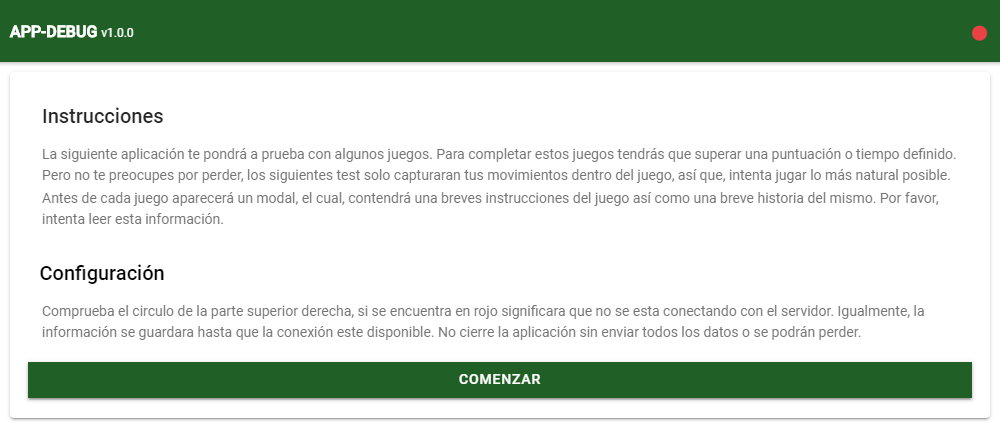
\includegraphics[width=0.8\textwidth, keepaspectratio]{imaxes/application/main_page.png}
    \caption{Ventana principal}
    \label{fig:main_page}
\end{figure}

\section{Configuración de la aplicación}

Para acceder a la pantalla de configuración es necesario realizar un patrón, que consiste en tocar las cuatro esquinas de la pantalla. Al realizar el patrón se mostrará la configuración de la aplicación [Figura~\ref{fig:config_page}]. En esta ventana se puede configurar algunos de los aspectos de la aplicación como tiempo de la aplicación y la dirección del servidor. Además de la configuración también se muestran los datos actuales de la aplicación y un registro de eventos.

\begin{figure}[!h]
    \centering
    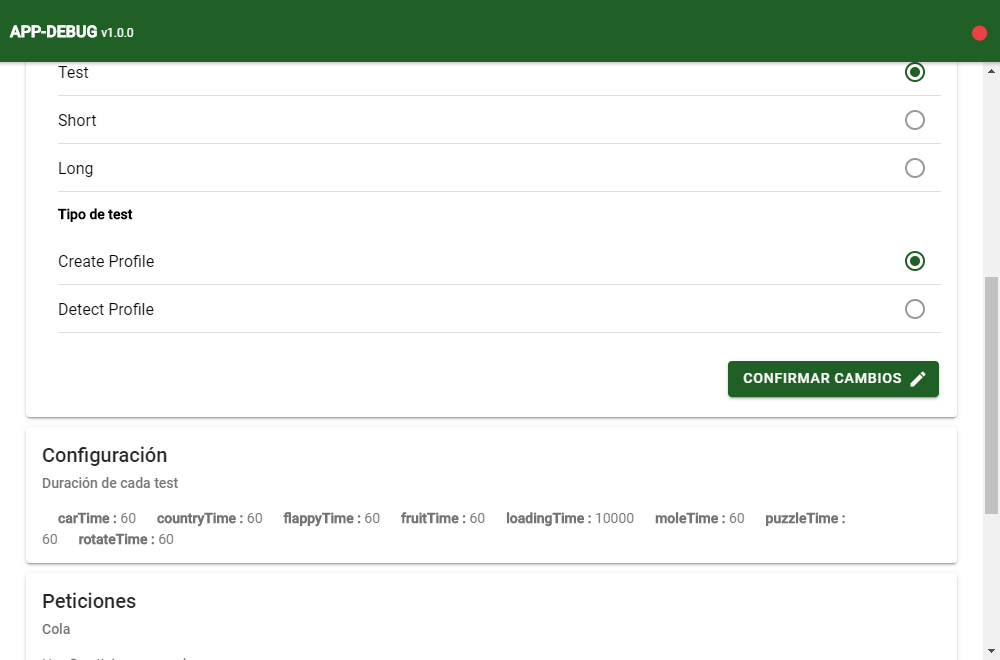
\includegraphics[width=0.8\textwidth, keepaspectratio]{imaxes/application/config_page.png}
    \caption{Menú de configuración}
    \label{fig:config_page}
\end{figure}

\newpage
\section{Inicio de la prueba}

Para iniciar la prueba solo es necesario presionar el botón \textbf{COMENZAR} y a continuación se abrirá un dialogo donde tendremos que introducir el nombre de usuario. [Figura~\ref{fig:login_page}]. 

\begin{figure}[!h]
    \centering
    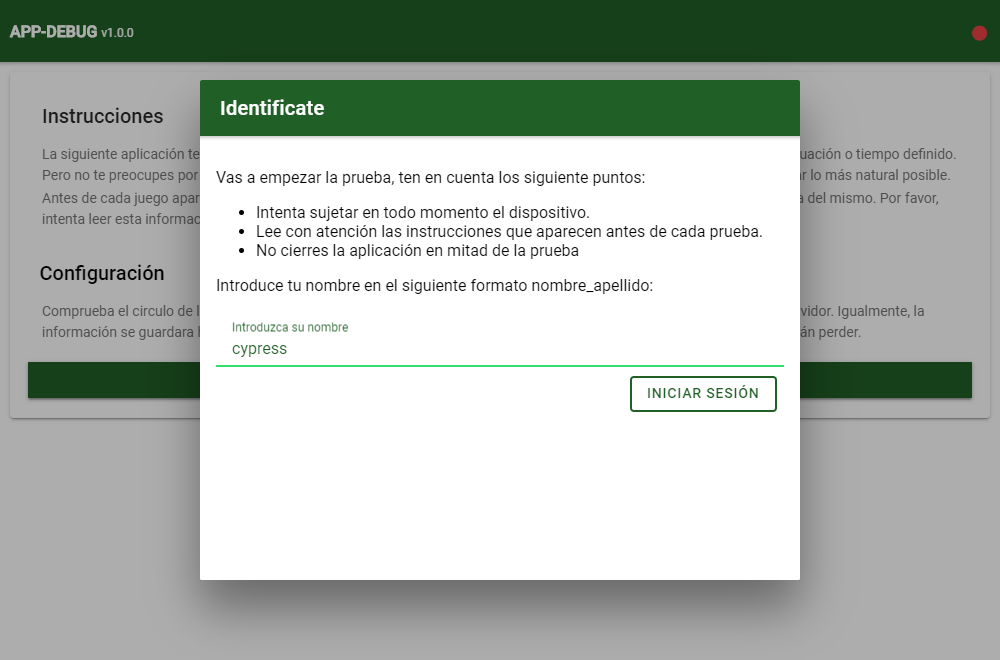
\includegraphics[width=0.6\textwidth, keepaspectratio]{imaxes/application/login_page.png}
    \caption{Ventana de login}
    \label{fig:login_page}
\end{figure}

\subsection{Desafíos}

\subsubsection{Puzzle Sliding}

Esta primera prueba [Figura~\ref{fig:puzzle_page}] consiste en resolver el puzzle que se muestra en pantalla, realizando movimientos de deslizamiento, en un tiempo límite establecido.

\begin{figure}[!h]
    \centering
    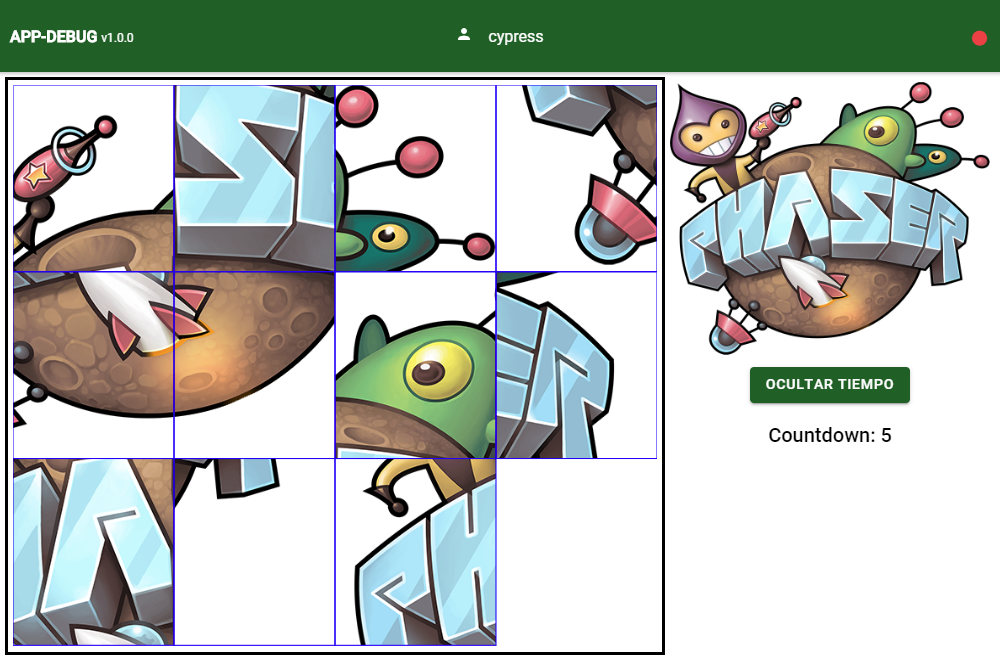
\includegraphics[width=0.6\textwidth, keepaspectratio]{imaxes/application/puzle-sliding-page.png}
    \caption{Ventana del juego de \textit{Puzzle Sliding}}
    \label{fig:puzzle_page}
\end{figure}

\subsubsection{Whack a mole}
En esta prueba [Figura~\ref{fig:mole_page}] tendremos que tocar la pantalla sobre los animales, los cuales aparecerán cada cierto tiempo.

\begin{figure}[H]
    \centering
    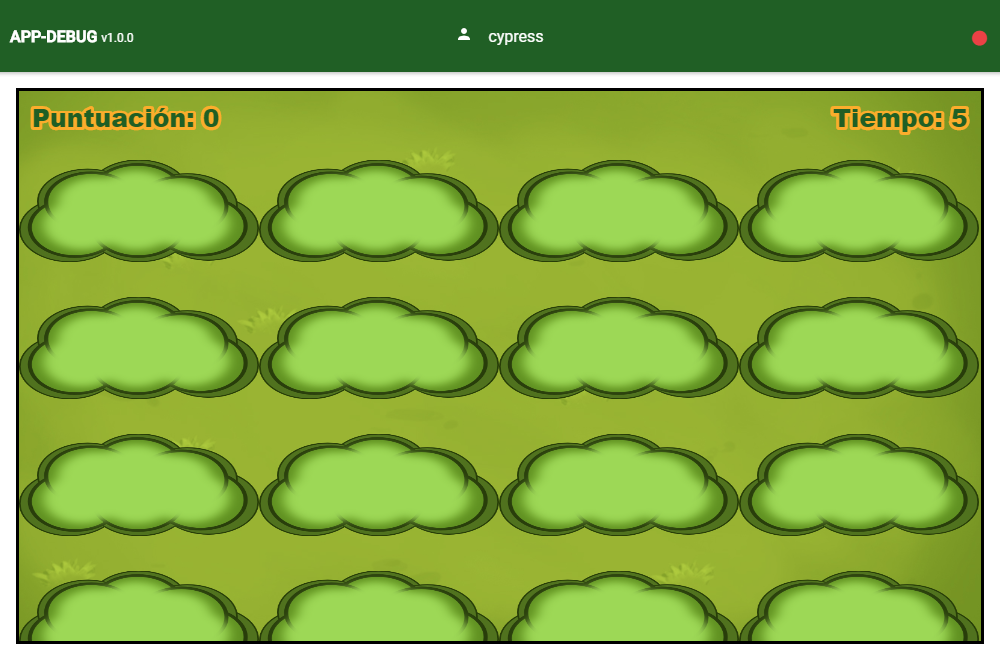
\includegraphics[width=0.7\textwidth, keepaspectratio]{imaxes/application/whack-mole-page.png}
    \caption{Ventana del juego de \textit{Whack a Mole}}
    \label{fig:mole_page}
\end{figure}

\subsubsection{Flappy Bird}
En esta prueba [Figura~\ref{fig:bird_page}] tendremos tocar la pantalla repetidamente, para intentar que el pájaro no choque contra las tuberías que irán apareciendo.

\begin{figure}[!h]
    \centering
    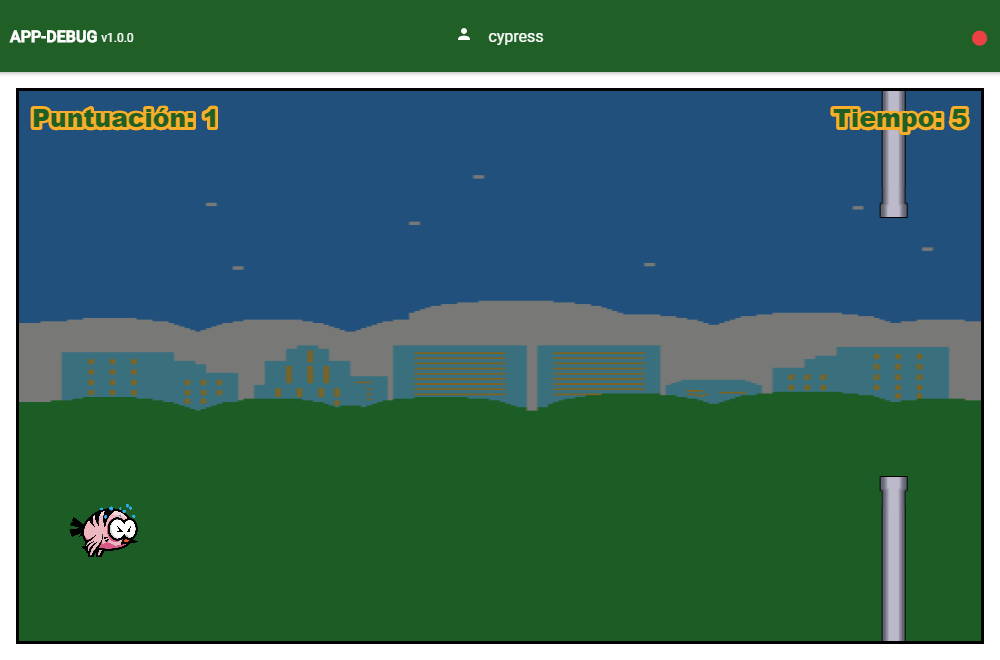
\includegraphics[width=0.7\textwidth, keepaspectratio]{imaxes/application/flappy-bird-page.png}
    \caption{Ventana del juego de \textit{Flappy Bird}}
    \label{fig:bird_page}
\end{figure}

\subsubsection{Fruit Ninja}
En esta prueba [Figura~\ref{fig:bird_page}] tendremos que delizar el dedo sobre la pantalla para cortar la fruta que vaya apareciendo.

\begin{figure}[!h]
    \centering
    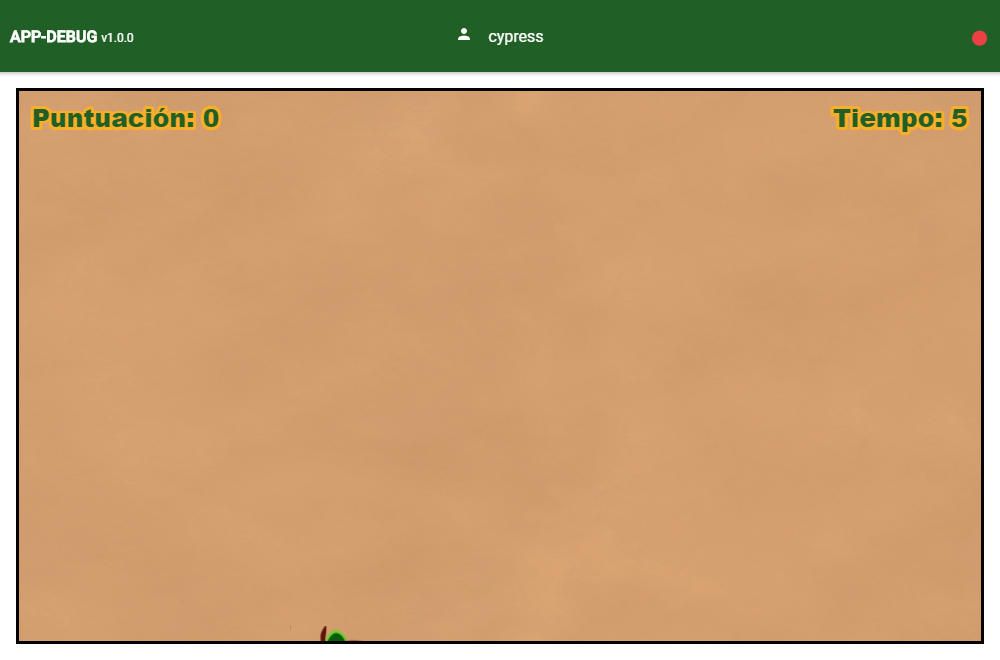
\includegraphics[width=0.7\textwidth, keepaspectratio]{imaxes/application/fruit-ninja-page.png}
    \caption{Ventana del juego de \textit{Fruit Ninja}}
    \label{fig:fruit_page}
\end{figure}

\subsubsection{Outrun}
En esta prueba [Figura~\ref{fig:bird_page}] tendremos que coger el dispositivo como si fuera el volante e intentar esquivar los obstaculos que irán apareciendo.

\begin{figure}[!h]
    \centering
    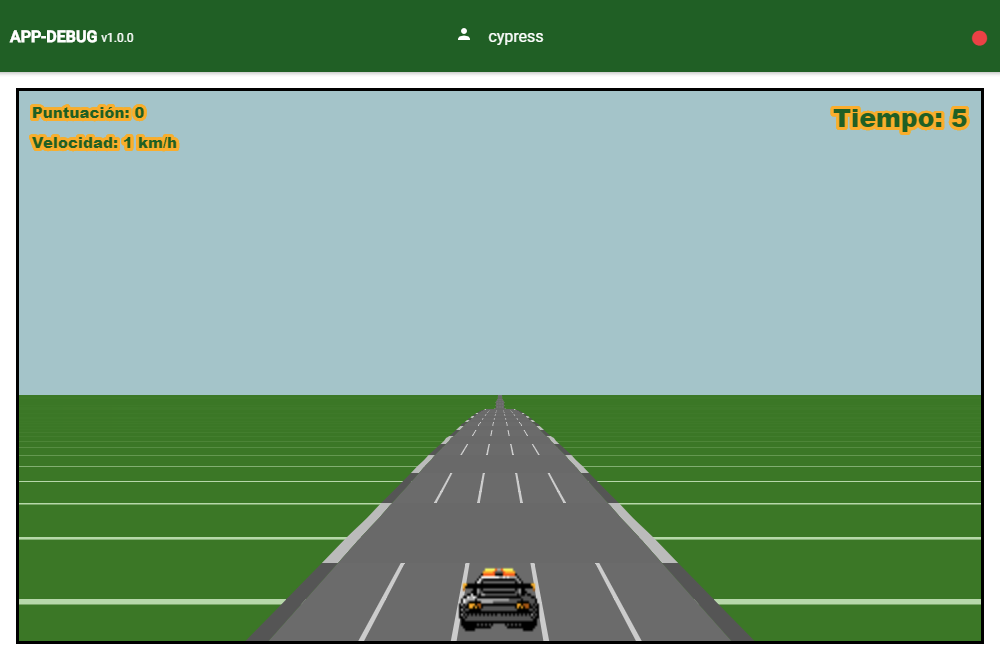
\includegraphics[width=0.7\textwidth, keepaspectratio]{imaxes/application/outrun-page.png}
    \caption{Ventana del juego de \textit{Outrun}}
    \label{fig:outrun_page}
\end{figure}

\subsubsection{Buscar Países}
En esta prueba [Figura~\ref{fig:search_page}] se nos muestra una lista de países ordenados alfabéticamente. El objetivo es buscar los países que se muestran en la parte superior izquierda.

\begin{figure}[!h]
    \centering
    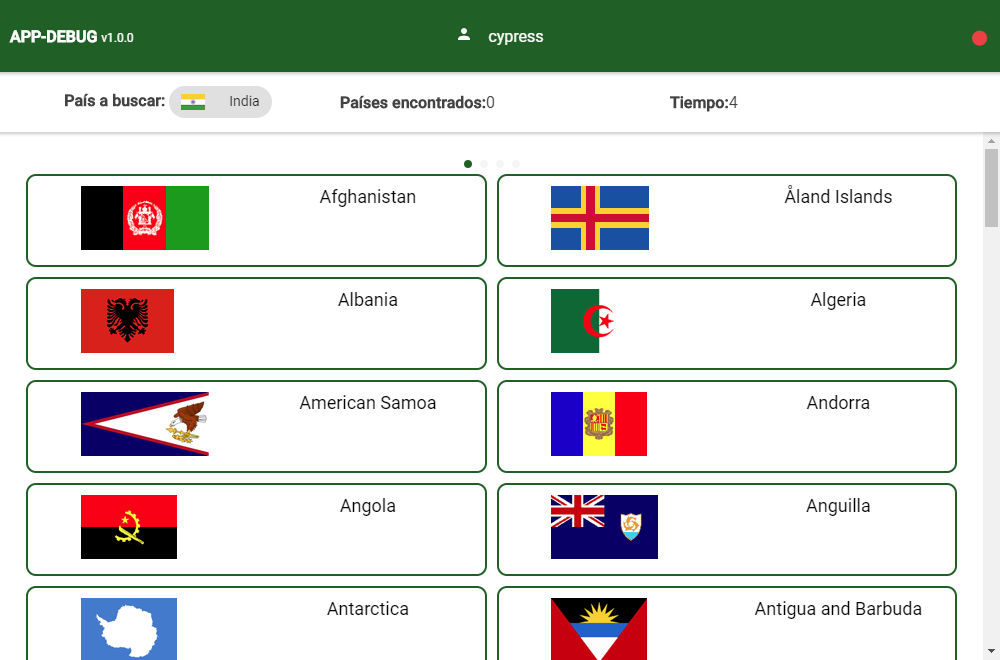
\includegraphics[width=0.7\textwidth, keepaspectratio]{imaxes/application/search-page.png}
    \caption{Ventana del juego de \textit{Buscar Países}}
    \label{fig:search_page}
\end{figure}

\subsubsection{Rotación}
En esta prueba [Figura~\ref{fig:rotate_page}] tendremos que hacer encajar las piezas y para ello tendremos que mover, rotar y escalar la pieza negra.

\begin{figure}[!h]
    \centering
    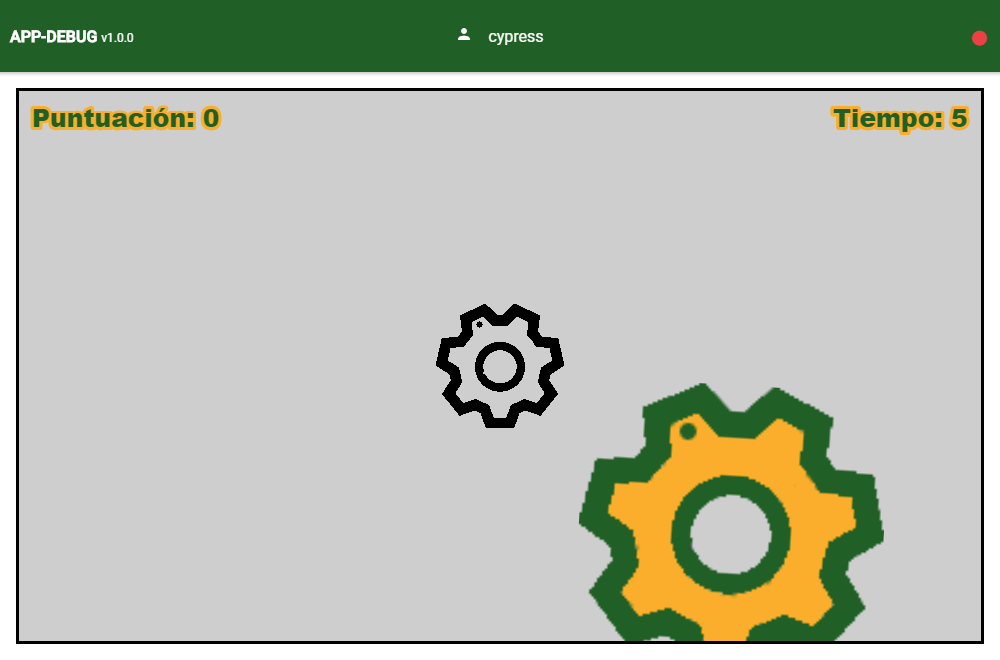
\includegraphics[width=0.7\textwidth, keepaspectratio]{imaxes/application/rotate-page.png}
    \caption{Ventana del juego de \textit{Rotación}}
    \label{fig:rotate_page}
\end{figure}


\subsection{Fin de la prueba}
Una vez finalizadas todas la pruebas la aplicación nos mostrara una tabla de puntuaciones [Figura~\ref{fig:score_page}] de todos los desafíos hechos. En esta ventana podremos volver al inicio pulsando el botón \textit{IR A INICIO}.

\begin{figure}[!h]
    \centering
    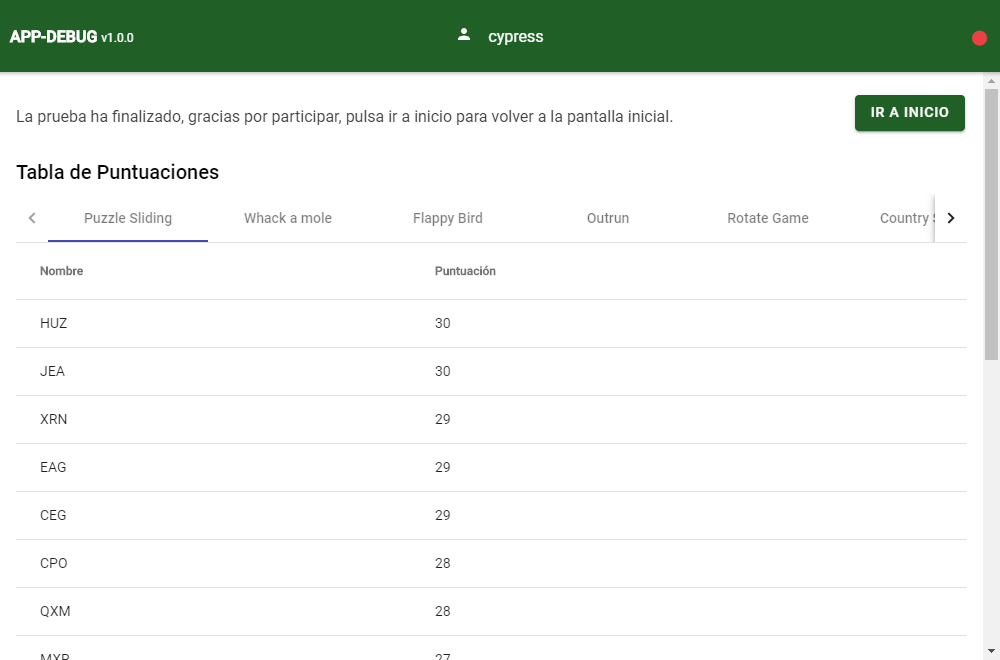
\includegraphics[width=0.7\textwidth, keepaspectratio]{imaxes/application/score-page.png}
    \caption{Ventana de puntuaciones}
    \label{fig:score_page}
\end{figure}

 \bibliographystyle{IEEEtran}
 \bibliography{\bibconfig,bibliografia/bibliografia}
 \cleardoublepage
 
\end{document}

%%%%%%%%%%%%%%%%%%%%%%%%%%%%%%%%%%%%%%%%%%%%%%%%%%%%%%%%%%%%%%%%%%%%%%%%%%%%%%%%
